%
% Datei: Studium/Diplomarbeit.tex
%
% Begonnen am: 18/01/97
%
\documentclass[twoside,12pt,a4paper]{report}
%\nofiles

\usepackage[latin1]{inputenc}
\usepackage[english,german]{babel}
\usepackage[T1]{fontenc}

% Computer Concrete Fonts verwenden
%\usepackage{ccfonts}
%\usepackage{em}
\usepackage{times}

\usepackage{typearea}\typearea[2cm]{14}
\usepackage{amsmath}
\usepackage{bm}
\usepackage[dvips]{graphicx}
\usepackage{subfigure}
\usepackage{float}
\usepackage{caption}
\renewcommand{\captionlabelfont}{\small\upshape\bfseries}
\renewcommand{\captionfont}{\small\slshape}
\usepackage{showkeys}
%\usepackage{showkeys}

\bibliographystyle{geralpha}

\makeatletter

\renewcommand\tiny{
   \@setfontsize\normalsize\@xivpt{18}%
   \abovedisplayskip 14\p@ \@plus3\p@ \@minus7\p@
   \abovedisplayshortskip \z@ \@plus3\p@
   \belowdisplayshortskip 6.5\p@ \@plus3.5\p@ \@minus3\p@
   \belowdisplayskip \abovedisplayskip
   \let\@listi\@listI}
\renewcommand\small{%
   \@setfontsize\normalsize\@xiipt{14.5}%
   \abovedisplayskip 12\p@ \@plus3\p@ \@minus7\p@
   \abovedisplayshortskip \z@ \@plus3\p@
   \belowdisplayshortskip 6.5\p@ \@plus3.5\p@ \@minus3\p@
   \belowdisplayskip \abovedisplayskip
   \let\@listi\@listI}
\renewcommand\footnotesize{%
   \@setfontsize\small\@xipt{13.6}%
   \abovedisplayskip 11\p@ \@plus3\p@ \@minus6\p@
   \abovedisplayshortskip \z@ \@plus3\p@
   \belowdisplayshortskip 6.5\p@ \@plus3.5\p@ \@minus3\p@
   \def\@listi{\leftmargin\leftmargini
               \topsep 9\p@ \@plus3\p@ \@minus5\p@
               \parsep 4.5\p@ \@plus2\p@ \@minus\p@
               \itemsep \parsep}%
   \belowdisplayskip \abovedisplayskip
}

\normalsize
\makeatother

% Vektoren werden fett geschrieben
\renewcommand{\vec}{\bm}

\newcommand{\siehe}{\ensuremath{\nearrow}}

% H�ufig ben�tigte Worte/Floskeln
%\newcommand{\aug}{\ifmmode{\mathrm{AuGa}_2}\else{AuGa$_2$}\fi}
\newcommand{\aug}{{AuGa\ensuremath{_2}}}
%\newcommand{\ga}{\ifmmode{^{69}\mathrm{Ga}}\else{$^69$Ga}\fi}
\newcommand{\ga}{{\ensuremath{^69}Ga}}
%\newcommand{\gb}{\ifmmode{^{71}\mathrm{Ga}}\else{$^71$Ga}\fi}
\newcommand{\gb}{{\ensuremath{^71}Ga}}
\newcommand{\Ha}{\ensuremath{{\cal H}}}
\newcommand{\K}{\ensuremath{{\cal K}}}

%%%%%%%%%%%%%%%%%%%%%%%%%%%%%%%%%%%%%%%%%%%%%%%%%%%%%%%%%%%%%%%%%%%%%%%%%%%%%%%%%%%%%%%%%%%%%%%%%%

% Bildbreiten:
\newlength{\ssmallwidth}
\setlength{\ssmallwidth}{0.5\textwidth}
\newlength{\smallwidth}
\setlength{\smallwidth}{0.6\textwidth}
\newlength{\midwidth}
\setlength{\midwidth}{0.7\textwidth}
\newlength{\bigwidth}
\setlength{\bigwidth}{0.8\textwidth}

%%%%%%%%%%%%%%%%%%%%%%%%%%%%%%%%%%%%%%%%%%%%%%%%%%%%%%%%%%%%%%%%%%%%%%%%%%%%%%%%%%%%%%%%%%%%%%%%%%

% quer: Setzt Strich "uber #1
\newcommand{\quer}[1]{\overline{#1}}
% ul: Unterstreicht #1
\newcommand{\ul}[1]{\ensuremath{\underline{\mathrm{#1}}}}

% Text in Formeln mit Raum vor (\beforetext) und nach (\aftertext) dem Text
\newcommand{\beforetext}{\quad}
\newcommand{\aftertext}{\quad}
\newcommand{\ttext}[1]{\beforetext\text{#1}} % Abstand nur vorher
\newcommand{\textt}[1]{\text{#1}\aftertext}  % Abstabd nur nachher
\newcommand{\ttextt}[1]{\beforetext\text{#1}\aftertext} % Abstand vor- und nachher

% "Betrag": schlie"st #1 in angepasste Striche | ein
\newcommand{\abs}[1]{\left\lvert \smash[t]{#1} \right\rvert}

% \log-like
\DeclareMathOperator{\Spur}{Spur}

%%%%%%%%%%%%%%%%%%%%%%%%%%%%%%%%%%%%%%%%%%%%%%%%%%%%%%%%%%%%%%%%%%%%%%%%%%%%%%%%%%%%%%%%%%%%%%%%%%
%\includeonly{Experimente}

\sloppy

\hyphenation{Abs-zis-sen-wert-te}

\begin{document}

\nocite{Abragam,Abragam2,HakenWolf1,HakenWolf2,Kittel,Gerthsen,Slichter,POBELL,Metallic,Girgl,ESKA89,BAEUML,ESKA86,
	Maenne_PhD,koerber91,herrmannsdoerfer96,Stephan_Dis,PhDS} 

\setlength{\parindent}{0em}
\setlength{\parskip}{1ex}

\tableofcontents
\chapter*{Einleitung und Motivation}
\addcontentsline{toc}{chapter}{Einleitung und Motivation}

AuIn$_2$ zeigt bei Temperaturen unterhalb 1~mK einige faszinierende kernmagnetische
Eigenschaften, die z.\ T. von der hohen Kernspinpolarisation der In"=Kerne initiiert 
werden. Die in \cite{Wagner_Dis} an verschieden vorbehandelten AuIn$_2$"=Proben durchgeführten
NMR"=Messungen zeigten ein schwer interpretierbares Verhalten, u.\ a.\ wurden stark
unterschiedliche Spin"=Spin Relaxationszeiten gemessen und an einer Probe sogar die Möglichkeit der Erzeugung
multipler Spin"=Echos festgestellt.

Mit den im Rahmen dieser Arbeit durchgeführten NMR"=Experimenten soll das zu AuIn$_2$ isostrukturelle
AuGa$_2$ untersucht werden. Die Vertreter der Klasse der intermetallischen Verbindungen AuX$_2$
(X=Al,Ga,In) liegen alle in der kubischen CaF$_2$ Struktur vor, in der die Atome des Elements X
auf einfach kubischen Gitterplätzen sitzen (siehe Abb.~\ref{fig:auga2}), was u.\ a.\ die
Unterdrückung der Quad\-ru\-pol\-auf\-spal\-tung der NMR"=Linien zur Folge hat.

Es ist von Interesse, inwieweit auch in \aug{} das Relaxationsverhalten der Ga"=Spins ähnlich zu
AuIn$_2$ durch die Spinpolarisation bei tiefen Temperaturen modifiziert wird und welche 
Erklärungen für das bei AuIn$_2$ beobachtete Verhalten gefunden werden können.

Wie schon seit den sechziger Jahren bekannt ist zeigt \aug, im Gegensatz zu den beiden anderen
AuX$_2$"=Verbindungen, aufgrund von Besonderheiten der Bandstruktur eine ungewöhnliche
Temperaturabhängigkeit der Suszeptibilität und der Knightshift, wobei letztere im
Temperaturbereich von 4.2 K bis 300 K sogar ihr Vorzeichen wechselt. \cite{AuGa2Dilemma}.

In \cite{Stephan_Dis} wird für \aug{} als Supraleiter 1. Art eine Sprungtemperatur von 1.05~K und
ein kritisches Feld von 7.6~mT bestimmt. Messungen der spezifischen Wärme bzw. der
kernmagetischen Resonanz an reinem Gallium haben gezeigt, daß für $T>500\;\mu$K keine
kernmagnetischen Anomalien auftreten. In \cite{Stephan_Dis} wurde die Ordnungstemperatur der
magnetischen Kermomente aufgrund der Dipol"=Dipol Wechselwirkung zwischen den Ga"=Kernen auf
$T_c^{DD}=0.20\;\mu$K abgeschätzt.

{\bfseries Hinweis: }
Im Weiteren wird $\vec B=\mu_r\mu_0\vec H$ das Magnetfeld genannt und in der Einheit "`Tesla"' angegeben.

\chapter{Theoretische Grundlagen}

\section{magnetische Kernspinresonanz}

Atomkerne mit einem Kernspin $\vec I$ besitzen ein dem Kernspin proportionales magnetisches Dipolmoment $\vec
\mu_I$:
	\[
		\vec \mu_I=\gamma\,\vec I
	\]
Dabei ist $\gamma$ ist das gyromagnetische Verhältnis (von Spin und magnetischem Moment). Die
Einheit des magnetischen Kernmoments ist, in Analogie zum Bohrschen Magneton $\mu_B$ der
Elektronen, das Kernmagneton $\mu_K$, das um das Verhältnis von Elektronen"= zu Protonenmasse
kleiner als $\mu_B$ ist.
	\[
		\vec\mu_I=\frac{g_I\,\mu_K}{\hbar}\vec I,\ttextt{mit}\mu_K=0.505\cdot10^{-26}\text{Am}^2
	\]
Man kann weiterhin in Analogie zu den Elektronen einen Kern"=$g$"=Faktor einführen, der durch
$g_I=(\gamma\;\hbar/\mu_K)$ definiert ist. Allerdings ergibt sich $g_I$ im Gegensatz zum
Landé"=$g_J$"=Faktor der Elektronenschalen nicht aus den das System beschreibenden
Quantenzahlen, sondern ist eine empirische, für jedes Nukleon charakteristische Meßgröße.

Für den Betrag des Drehimpulses des Kerns gilt:
	\[
		\abs{\vec I}=\sqrt{I(I+1)}\;\hbar
	\]
Die so definierte Kernspinquantenzahl $I$ ist ganz oder halbzahlig.

Meßbar ist nur die Komponente von Spin und magnetischem Moment in der Vorzugsrichtung, die durch
die Richtung eines von außen angelegten Magnetfeldes $\vec B_0$ vorgegeben ist. Im Weiteren ist
die Richtung der $z$"=Achse im Koordinatensystem immer durch diese Vorzugsrichtung festgelegt. Für
die Komponenten von Kernspin und magnetischem Moment parallel zu dieser Vorzugsrichtung gilt
dann:
	\[
		I_z = m_I\;\hbar\ttextt{und}\mu_z=\gamma\;\hbar m_I=g_I\mu_Km_I
	\]
Hierbei ist $m_I$ die magnetische Quantenzahl des Kernspins. Sie kann Werte im Intervall $[-I,
-I+1, \ldots, I-1, I]$ annehmen und repräsentiert die $(2I+1)$"=fache Möglichkeit der Einstellung
der $z$"=Komponente des Kernspins relativ zur Vorzugsrichtung. Die Vorzeichen des magnetischen
Moments $\vec\mu_I$ und des $g_I$"=Faktors können positiv oder negativ sein.

In einem äußeren Magnetfeld $\vec B_0$ besitzt ein Kern aufgrund seines magnetischen Moments die
magnetische Wechselwirkungsenergie (Zeemann"=Energie)
	\[
		V=-\vec \mu_I\cdot\vec B_0=-g_I\,\mu_K\,B_0\,m_I\ttext{.}
	\]
Diese äquidistanten Energieniveaus sind im thermischen Gleichgewicht nach der Boltzmannverteilung
\eqref{eqn:boltzmann} besetzt. Die Energiedifferenz zwischen zwei benachbarten
Einstellmöglichkeiten des magnetischen Moments im Feld $\vec B_0$ und damit die Energie für Dipolübergänge
mit $\Delta m_I=\pm1$, beträgt demnach
	\[
		\Delta E=g_I\,\mu_K\,B_0\ttext{.}
	\]
Strahlt man auf eine Probe, senkrecht zu $\vec B_0$ elektromagnetische Wellen ein, die die
Resonanzbedingung
	\begin{equation}
		\label{eqn:resonanzbed}
		\omega=\frac{\Delta E}{\hbar}=\frac{g_I\,\mu_K}{\hbar}B_0
	\end{equation}
erfüllen, so kann diese Strahlung von der Probe absorbiert werden und somit magnetische
Dipolübergänge zwischen den möglichen Kernspin"=Orientierungen induzieren. Diesen Prozeß nennt man
Kernspin"=Resonanz. Diese Resonanz bedeutet ein Übereinstimmen der Frequenz der eingestrahlten
Strahlung mit der Larmor"=Präzessionsfrequenz, mit der die Kernspins im Magnetfeld $\vec B_0$ um
dessen Richtung präzedieren.

Der Vorteil der Resonanzmethode besteht darin, daß der Anteil der Kernsuszeptibilität an der
Gesamtsuszeptibilität selektiv betrachtet werden kann, auch wenn ihr Beitrag relativ klein ist.
Zusätzlich liefert die NMR aus den meßbaren Relaxationszeiten Informationen über
Wechselwirkungsprozesse, die auf atomarem Niveau ablaufen.

Man unterscheidet zwei Methoden der Bestimmung von NMR"=Spektren:
	\begin{itemize}
		\item Eine Möglichkeit, NMR"=Spektren aufzunehmen, ist die Methode der
			\emph{cw"=Kernspinresonanz} (cw = \ul{c}ontinuous
			\ul{w}ave). Hierbei wird über die Probenspule ständig ein schwaches Hochfrequenzsignal
			eingestrahlt. Man kann nun entweder die Frequenz des schwachen Hochfrequenzsignals
			langsam ändern oder durch Änderung der Stärke des äußeren Feldes $B_0$ nach Gleichung 
			\eqref{eqn:resonanzbed} die NMR"=Resonanzfrequenzen relativ zur eingestrahlten Frequenz
			verändern. Das Resonanzspektrum wird durch Messung der
			Energieabsorption in der NMR"=Spule in Abhängigkeit von der angeregten Frequenz oder
			der Magnetfeldstärke aufgenommen.
		\item Für die Messungen im Rahmen dieser Arbeit wurde die Methode der \emph{gepulsten
			Kernspinresonanz} verwendet. Hierbei wird senkrecht zum Feld $\vec B_0$ ein Hochfrequenzpuls
			der Amplitude $B_\mathrm{HF}$ für die Zeit $t_\mathrm{Puls}$ mit Hilfe einer Spule in die Probe eingestrahlt
			(siehe dazu auch Abb.~\ref{fig:probe} auf Seite~\pageref{fig:probe}).
			Nach Pulsende verwendet man dieselbe Probenspule dazu, um Änderungen
			des magnetischen Flusses in Spulenrichtung zu detektieren. Nach dem HF"=Puls erhält man
			eine makroskopisch meßbare Komponente der Probenmagnetisierung senkrecht zu $\vec
			B_0$. Die makroskopische Magnetisierung präzediert somit mit der Larmorfrequenz um die
			Richtung von $\vec B_0$. Das führt dazu, daß sich der magnetische Fluß durch die
			Probenspule periodisch ändert. Die in der Probenspule induzierte Spannung ist somit
			proportional zur Änderung des magnetischen Flusses in Spulenrichtung. Dieses Signal,
			daß proportional zur zeitlichen Änderung der Probenmagnetisierung in Spulenrichtung
			ist, nennt man den freien Induktionszerfall (auch \ul{f}ree \ul{i}nduction \ul{d}ecay,
			{\bfseries FID}). Das NMR"=Resonanzspektrum kann man durch Fouriertransformation aus
			dem aufgezeichneten FID ermitteln.
	\end{itemize}

Als Modell für die \emph{gepulste Kernspinresonanz} kann man die Schrödingergleichung für
einen freien Spin $I=\frac12$ in einem konstanten Magnetfeld $\vec B_0$ und einem schwachen dazu
senkrechten zeitabhängigen Magnetfeld lösen.
Dieses zeitabhängige Magnetfeld rotiert mit der Amplitude $B_\mathrm{HF}$ und der Larmorfrequenz
$\omega_0=\frac{g_I\mu_KB_z^0}{\hbar}$ in der $xy$"=Ebene. Die Schrödingergleichung lautet dann:
	\begin{equation}
		\left(-\vec\mu\cdot{\vec B}\right) \phi = i\;\hbar \frac{d\phi}{dt}
	\end{equation}
mit
	\[
			\vec B= \begin{pmatrix}0\\0\\B_z^0\end{pmatrix}+
					\begin{pmatrix}B_x^s(t)\\B_y^s(t)\\0\end{pmatrix}
	\ttextt{und}
		\begin{matrix}
			B_x^s(t) = B_\mathrm{HF}\cos(\omega_0t)\\ 
			B_y^s(t) = B_\mathrm{HF}\sin(\omega_0t)
		\end{matrix}
	\]
Mit $\Omega=\frac{\mu_I\mu_K}{\hbar}B_\mathrm{HF}$ kann man nun die zeitliche Entwicklung der
Erwartungswerte der Spinkomponenten und somit auch der des magnetischen Moments herleiten:
	\begin{equation}
		\label{eqn:s_xyz}
		\begin{array}{rl}
			\left<\mu_x\right>&=-\frac{\gamma\;\hbar}2\sin(\Omega t)\sin(\omega_0t)\\
			\left<\mu_y\right>&=\phantom{-}\frac{\gamma\;\hbar}2\sin(\Omega t)\cos(\omega_0t)\\
			\left<\mu_z\right>&=-\frac{\gamma\;\hbar}2\cos(\Omega t)
		\end{array}
	\end{equation}
Wie man sieht, beschreiben $\cos(\Omega t)$ und $\sin(\Omega t)$ die Auslenkung der
Gleichgewichtsmagnetisierung aus der z"=Richtung, den sog.\ \emph{Tippingwinkel} $\theta$. Dieser ist
danach proportional zum Produkt aus der Amplitude und der Zeitdauer des HF"=Pulses:
	\begin{equation}
		\theta_\mathrm{tip} = \Omega t_\mathrm{Puls}
			= \frac{\mu_I\mu_K}{\hbar}B_\mathrm{HF}t_\mathrm{Puls}
	\end{equation}
Die Terme $\sin(\omega_0t)$ und $\cos(\omega_0t)$ beschreiben die Larmorpräzession des
magnetischen Moments in der $xy$"=Ebene.

Wenn man die Zeitableitung der Gleichungen \eqref{eqn:s_xyz} bildet, erhält man die
Bewegungsgleichung für die Erwartungswerte des magnetischen Moments:
	\begin{equation}
		\frac{d}{dt}\left<\vec \mu\right>=\gamma\left<\vec\mu\right> \times \vec B(t)\ttext{.}
	\end{equation}

Diese Gleichung, die für eine beliebige Zeitabhängigkeit des Magnetfeldes $\vec B(t)$ gültig
ist, erinnert an die Kreiselgleichung der klassischen Mechanik. Das magnetische Moment $\vec \mu$
präzediert also im Magnetfeld $\vec B(t)$.

Wenn man nun zu einem Ensemble von zunächst ungekoppelten Spins übergeht, gilt diese Gleichung
aufgrund der Statistik auch für die mittlere Magnetisierung dieses Ensembles. Berücksichtigt man
nun, daß die Kernspins untereinander und mit ihrer Umgebung wechselwirken, kann man zur
Beschreibung dieser Wechselwirkung phänomenologische Relaxationsterme einzuführen. Diese enthalten
zum einen die Wechselwirkung der Kernspins untereinander und zum anderen die Wechselwirkung der
Kernspins mit dem sie umgebenden Wärmebad (z.\ B. Leitungselektronen, Kristallgitter \ldots).
Daraus ergibt sich die im folgenden Abschnitt behandelte Blochgleichung.

%%%%%%%%%%%%%%%%%%%%%%%%%%%%%%%%%%%%%%%%%%%%%%%%%%%%%%%%%%%%%%%%%%%%%%%%%%%%%%%%%%%%%%%%%%%%%%%%%%

\section{Die phänomenologische Blochgleichung}
\label{sec:blocheqn}

Für die mittlere Magnetisierung eines Ensembles von Kernspins gilt die phänomenologische
Blochgleichung:

\begin{equation}
	\label{eqn:bloch}
	\dot{\vec M} = \underbrace{\gamma {\vec M} \times \vec B_\mathrm{eff}}_1
				 - \underbrace{\frac{M_x \vec e_x + M_y \vec e_y}{T_2}}_2
				 - \underbrace{\frac{M_0-M_z}{T_1}\vec e_z}_3
\end{equation}
Die einzelnen Terme haben folgende Auswirkungen auf die zeitliche Entwicklung der Magnetisierung:
\begin{description}
	\item[Term 1:] {\bfseries Präzession der Magnetisierung um das effektive Magnetfeld.}
		\begin{description}
			\item[$B_\mathrm{eff}$:] effektives Magnetfeld am Kernort, eine genaue Beschreibung
				befindet sich im Abschnitt \ref{ssec:beff}.
			\item[$\gamma$:] gyromagnetisches Verhältnis $\gamma=\frac{g_I\mu_K}{\hbar}$
		\end{description}

		Die Magnetisierung $\vec M$ präzediert mit $\omega=\gamma \abs{\vec
		B_\mathrm{eff}}=\frac{g_I\mu_K}{\hbar}\abs{\vec B_\mathrm{eff}}$ um die Richtung von $\vec
		B_\mathrm{eff}$.
	\item[Term 2:] {\bfseries Abklingen der Quermagnetisierung.}

		Werden durch den HF"=Puls Komponenten $\vec M_x$ und $\vec M_y$ von $\vec M$ erzeugt,
		präzedieren diese nach Term 1 um $\vec B_\mathrm{eff}$.
		Infolge von Fluktuationen des lokalen Feldes geraten die Kernspins wegen der daraus
		resultierenden leicht unterschiedlichen Präzessionsfrequenzen außer
		Phase. Da man mit der NMR"=Spule den Mittelwert der Magnetisierung aller Spins
		mißt, führt dies zum Abklingen der gemittelten Beiträge von $\vec M_x$ und $\vec M_y$.

		Das Abklingen der Quermagnetisierung wird durch $T_2$ beschrieben. Dies ist die
		\emph{transversale Relaxationszeit} (auch \emph{intrinsische
		Spin"=Korrelationszeit} oder \emph{Spin"=Spin Relaxationzeit}). Die Gesamtenergie des
		Spinsystems bleibt für Spin"=Spin"=Relaxationsprozesse im statischen Magnetfeld erhalten; es
		ist somit kein Energieaustausch mit einem Energiereservoir notwendig (vgl. dazu den
		$T_1$"=Zerfall mit Energietransport beschrieben in Kap.~\ref{sec:sgrelax}).

		Die Wahl eines exponentiellen Zerfallsgesetzes der Quermagnetisierung ist nur eine
		Näherung, die aber zur Beschreibung wichtiger Effekte ausreicht. Der Mechanismus der
		Spin"=Spin"=Relaxation in einem Festkörper ist die Verteilung der Präzessionsfrequenzen im
		Magnetfeld der Nachbaratome. Man erklärt dies durch ein lokales Feld $\vec
		B_\mathrm{loc}$, das von den magnetischen Momenten der Nachbaratome stammt und das
		entweder dem äußeren statischen Feld $\vec B_0$ entgegengesetzt oder ihm gleichgerichtet
		ist. Zusätzlich existiert noch ein fluktuierender, zu $\vec B_0$ senkrechter Anteil, der
		die Ursache für auftretende Spin"=Übergänge darstellt (siehe auch
		Abschnitt~\ref{sec:sgrelax}). Die Auswirkung dieses lokalen Feldes ist eine merkliche
		Dephasierung der präzedierenden Kernspins nach einer Zeit, die in der Größenordung
		$\frac1{\gamma B_\mathrm{loc}}$ liegt. Als grobe Abschätzung erhält man somit für $T_2$
			\begin{equation}
				T_2=\frac1{\gamma B_\mathrm{loc}}\ttext{.}
			\end{equation}
		Bei Metallen ist $T_2$ meist in der Größenordnung $100$~µs.

		Ein möglicher theoretischer Zugang zur Linienform der Resonanzlinie ist die Berechnung von
		Momenten $M_n$ des Resonanzlinienspektrums $f(\omega)$ mit dem Maximum bei $\omega_0$
		\cite[S. 106ff]{Abragam}:
			\begin{equation}
				M_n = \int(\omega-\omega_0)^n\,f(\omega)\,d\omega
			\end{equation}

Man kann diese Momente mittels Störungsrechnung $\Ha=\Ha_0+\Ha_1$ für ein System aus identischen,
über die Dipol"=Dipol"=Wechselwirkung wechselwirkenden Kernspins berechnen. Wenn man nur den
säkularen Teil des Störoperators $\Ha_1$ verwendet, der mit dem ungestörten Operator $\Ha_0$
kommutiert, kann man die geraden Momente $M_2$, $M_4$, usw.\ berechnen. Hierbei erhält man auch,
daß NMR"=Resonanzlinien immer symmetrisch sind und somit sind alle ungeraden Momente $M_1$, $M_3$,
\ldots identisch 0.

		Ein vorhandener Feldgradient des statischen Feldes $B_0$ führt zu einer zusätzlichen
		Verstärkung der Dephasierung der Kernspins. Dies muß dann
		berücksichtigt werden, falls die Spin"=Spin Relaxationzeit aus der Linienbreite der
		Resonanzlinie bestimmt werden soll. Der Gradient des Magnetfeldes $\Delta B_0$ führt zu
		einer effektiven Spin"=Spin Relaxationzeit $T_2^\ast$ von:
			\begin{equation}
				\label{eqn:t2stern}
				\frac1{T_2^\ast}=\frac1{T_2}+\gamma\,\Delta B_0
			\end{equation}	
		Darum wird $T_2$ nicht aus der Linienbreite der Resonanzlinie, sondern mit Hilfe
		der Spin"=Echo"=Methode ermittelt. Hierbei hat die reversible Dephasierung, die
		durch den Gradienten von $\vec B_0$ verursacht wird, keinen Einfluß auf das Meßergebnis.
		(siehe die Messung der Spin"=Spin Relaxationzeit in Abschnitt~\ref{sec:messungt2})

		Allerdings ist es umgekehrt mittels \eqref{eqn:t2stern} möglich, bei bekanntem $T_2$ den Magnetfeldgradienten am Probenort aus der
		Linienbreite der Resonanzlinie zu bestimmen.

	\item[Term 3:] {\bfseries zeitliche Entwicklung der Magnetisierung in Richtung von $\vec B_0$}
		hin zum thermodynamischen Gleichgewichtswert
		$M_0 \vec e_z=M_\mathrm{sat}P\left(\frac{B_0}{T}\right)\vec e_z$, wobei
		$P\left(\frac{B_0}{T}\right)$ die durch Gleichung \eqref{eqn:polarisation} definierte
		Polarisation des Kernspinsystems darstellt.

		$T_1$ ist dabei die \emph{longitudinale Relaxationszeit} oder auch
		\emph{Spin"=Gitter Relaxationzeit}. (siehe Abschnitt \ref{sec:sgrelax})
\end{description}

\subsection{effektives Feld am Kernort}
\label{ssec:beff}

Das auf die magnetischen Kernmomente wirkende effektive Magnetfeld setzt sich aus folgenden
Komponenten zusammen:

\begin{equation}
	\vec B_\mathrm{eff} = \vec B_0 + \vec B_\mathrm{HF}(t) + \mu_0\left[\tilde{L} - \tilde{N} + \tilde{\lambda}\right]\vec M
\end{equation}

Dabei ist:

\begin{description}
	\item[$\vec B_0$:] \emph{äußeres statisches Feld}. Bei den hier durchgeführten Messungen ist es
		der größte Beitrag zum effektiven Feld und bestimmt somit nach \eqref{eqn:resonanzbed} die Lage der Resonanzlinien im
		Spektrum. (Die hier vorgestellten Messungen wurden in Feldern $B_0$ im Bereich von 80 bis 800mT
		durchgeführt) 
	\item[$\vec B_\mathrm{HF}(t)$:] \emph{von außen eingestrahltes magnetisches Wechselfeld}.
		Dieses wird durch die NMR"=Spule, in der sich die Probe befindet, erzeugt. Die
		Achse dieser Spule ist senkrecht zur Richtung des äußeren statischen Magnetfeldes $\vec
		B_0$. (Die Größenordnung der Stärke des magnetischen Wechselfeldes liegt bei den
		durchgeführten Messungen mit gepulster NMR im Bereich einiger mT). Da es sich hier um eine
		massive Metallprobe handelt, dringt das über die NMR"=Spule eingestrahlte
		elektromagnetische Hochfrequenzfeld aufgrund des Skineffekts jedoch nur in
		eine dünne Oberflächenschicht der Probe ein. Die Dicke dieser Oberflächenschicht ist durch die frequenzabhängige Eindringtiefe
		der elektromagnetischen Wellen vorgegeben. Das Auftreten des Skineffekts hat zur Folge, daß die Anregung des
		Spinsystems nicht homogen erfolgt. Sie ist aufgrund der Abschwächung des HF"=Feldes abhängig vom Abstand zur Probenoberfläche.
		Man kann also nicht von einer homogenen Verteilung des Tippingwinkels nach dem Puls
		sprechen. Es bildet sich vielmehr eine Verteilung der Auslenkung der Kernspins
		aus, deren Struktur nicht mit einfacher Theorie zu erfassen ist.
	\item[$\vec B_N=\mu_0\tilde{N}\vec M$:] \emph{Entmagnetisierungsfeld}. Die magnetischen Dipole der
		Probe erzeugen ein dem Außenfeld $\vec B_0$ entgegengerichtetes und somit
		entmagnetisierendes Feld. Dieses ist von der Probenform abhängig und ist für einfache
		Geometrien analytisch berechenbar.
	\item[$\vec B_L=\mu_0\tilde{L}\vec M$:] Das \emph{Lorentzfeld} stellt einen Korrekturterm für $\vec B_N$
		dar, der daraus resultiert, daß in der unmittelbaren Umgebung jedes magnetischen Moments
		die Diskontinuität des Gitters aufgrund der Lokalisierung der Momente an diskreten
		Gitterplätzen berücksichtigt werden muß.

		Es wird der Anteil des homogenen entmagnetisierenden Feldes in einer Kugel um
		ein magnetisches Moment im Kristallgitter abgezogen und die Summe
		über die in der Kugel enthaltenen diskreten Momente $\vec b_i$ addiert.
		\begin{equation}
			\vec B_L = \sum_\mathrm{Kugel}\vec b_i - \mu_0\frac13\vec M
		\end{equation}
		Die Summe über die Kugel ist von der jeweiligen Gittersymmetrie abhängig und verschwindet
		z.\ B. für ein \emph{fcc}"=Gitter.

		Man kann auch einen korrigierten Entmagnetisierungstensor $\tilde{D}=\tilde{L}-\tilde{N}$
		einführen, der das effektive Entmagnetisierungsfeld beschreibt.

	\item[$\vec B_A=\mu_0\tilde{\lambda}\vec M$:] Das \emph{Austauschfeld}. Dieser Term beschreibt den
		Beitrag der indirekten Austauschwechselwirkung (auch Ruderman"=Kittel"=Wechselwirkung) zu den
		internen Feldern.

		Die langreichweitige indirekte Austauschwechselwirkung zwischen Kernspins wird durch
		Leitungselektronen vermittelt, die Wellenfunktionen mit $s$"=Charakter besitzen. Diese
		sind mit den Kernspins über die Fermi"=Kontakt"=Wechselwirkung gekoppelt.
\end{description}

Die inneren Felder wirken über den Larmorpräzessionsterm in der Blochgleichung \eqref{eqn:bloch}
auf das zeitliche Verhalten von $\vec M$. Falls jedoch der Entmagnetisierungstensor $\tilde{D}$
und der Austauschtensor $\tilde{\lambda}$ im Falle isotroper innerer Felder durch jeweils eine
skalare Größe ersetzt werden können, verschwindet deren Einfluß auf die Magnetisierung (da in
diesem Falle $\vec M\times\vec M=0$ gilt).

\subsection{Die Blochgleichungen in einem Mehrisotopensystem}

In einem Mehrisotopensystem, wie z.\ B. $^{69}$Ga und $^{71}$Ga in \aug{} und $^{63}$Cu und
$^{65}$Cu in der NMR"=Spule, werden die Abhängigkeiten der Magnetisierung untereinander
komplizierter. Das gekoppelte Gleichungssystem der Blochgleichung muß in diesem Fall
selbstkonsistent gelöst werden. Vor allem bei starker Austauschkopplung, die durch den Parameter
$\tilde{\lambda}$ repräsentiert wird, ergeben sich signifikanten Änderungen im NMR"=Verhalten bei
tiefen Temperaturen.


%%%%%%%%%%%%%%%%%%%%%%%%%%%%%%%%%%%%%%%%%%%%%%%%%%%%%%%%%%%%%%%%%%%%%%%%%%%%%%%%%%%%%%%%%%%%%%%%%%

\section{Die Brillouinfunktion und das Curie"=Gesetz}

Aus der Zustandssumme für ein Ensemble nicht wechselwirkender freier Spins im Magnetfeld ergibt
sich mit den Substitutionen $b:=g_I\mu_K B$ und $\beta:=\frac1{k_BT}$:
	\begin{equation}
		Z = \sum_{m=-I}^{+I}e^{-\beta bm} = e^{\beta bS}\sum_{j=0}^{2I}\left(e^{-\beta b}\right)^j = 
			\frac{\sinh\left(\beta b\left(I+\frac12\right)\right)}{\sinh\left(\beta \frac{b}2\right)}
	\end{equation}
Wie aus der statistischen Thermodynamik bekannt, erhält man den Erwartungswert des magnetischen
Moments in der Vorzugsrichtung $\vec e_z$ aus der gewichteten Summe
	\begin{equation}
		\frac1{Z}\sum_{m=-I}^{+I}\mu_z(m)\,e^{-\beta\cdot E(\mu_z(m))}
	\end{equation}
über die möglichen Energieniveaus. Wenn man
diese Summe noch umformt und mit Hilfe der freien Energie $F=-k_BT\ln(Z)$ vereinfacht, erhält
man:
	\begin{align}
		\left<\mu_z\right>&=\frac1{Z}\sum_{m=-I}^{+I}\mu_z(m)\,e^{-\beta(-\mu_z(m)B)}=
			-\frac{\partial F}{\partial B} = -\frac{\partial b}{\partial B}\frac{\partial F}{\partial b}\\
		&= g \mu_B\left(I+\frac12\right)\coth\left(\beta\left(I+\frac12\right)b\right)-\frac12g_I\mu_K\coth\left(\frac{\beta}2b\right)
	\end{align}
Man führt nun die Definition der \emph{Brillouinfunktion}
	\begin{equation}
		\label{eqn:brillouin}
		B_I(x) = \frac{2I+1}{2I}\coth\left(\frac{2I+1}{2I}x\right)-\frac1{2I}\coth\left(\frac1{2I}x\right)
	\end{equation}
ein, und kann damit den Mittelwert der Magnetisierung in $z$"=Richtung sehr einfach als
	\begin{equation}
		\left<\mu_z\right> = g_I\mu_KI\,B_I\left(\frac{g_I\mu_KI}{k_B}\,\frac{B}{T}\right)
	\end{equation}
ausdrücken. Da sich der Wertebereich der Brillouinfunktion von 0 (für
$\frac{B}{T}\rightarrow\infty$) bis 1 (für $\frac{B}{T}\rightarrow0$) erstreckt, ist die
Sättigungsmagnetisierung eines Spins gleich dem Vorfaktor $M_\mathrm{Sat}=g_I\mu_KI$
und die Polarisation der magnetischen Momente durch
	\begin{equation}
		\label{eqn:polarisation}
		P\left(\frac{B}{T}\right) = B_I\left(\frac{g_I\mu_KI}{k_B}\,\frac{B}{T}\right)
	\end{equation}
gegeben.

Man sieht hier, daß die mittlere Magnetisierung in $z$"=Richtung nur vom Quotienten $\frac{B}{T}$
abhängt. Für hohe Temperaturen $T$ und kleine Felder $B$ (d.\ h.\ $\frac{B}{T}\rightarrow0$
$\Rightarrow$ sehr kleine Polarisation) ist die
Entwicklung der Brillouinfunktion bis zur 1. Ordnung:
	\begin{equation}
		\left<\mu_z\right>
			=\frac{g_I^2\mu_K^2I^2}{k_B} \left(\frac12\frac{(2I+1)\left(\frac13I+\frac16\right)}{I}-\frac1{12}\frac1{I}\right)\frac{B}{T}
			+ O\left(\left(\frac{B}{T}\right)^2\right)
	\end{equation}
Daraus folgt für die Abhängigkeit von $T$
	\begin{equation}
		\label{eqn:curie}
		\left<\mu_z\right> \propto \frac1{T}\quad\Leftrightarrow\quad\left<\mu_z\right>=c_\mathrm{Curie}\frac1{T}
	\end{equation}
Dies ist das bekannte, für kleine Polarisation gültige \emph{Curie"=Gesetz}, das auch für die
makroskopische Magnetisierung gilt.

%%%%%%%%%%%%%%%%%%%%%%%%%%%%%%%%%%%%%%%%%%%%%%%%%%%%%%%%%%%%%%%%%%%%%%%%%%%%%%%%%%%%%%%%%%%%%%%%%%

\section{Die thermische Spin"=Gitter"=Relaxation}
\label{sec:sgrelax}


Im Folgenden wird nun diskutiert, wie die Kerne ihre thermische Gleichgewichtsmagnetisierung
infolge der Spin"=Gitter Relaxation erreichen. In dem Fall der Metalle bei tiefen Temperaturen kann
man von der Relaxation, die durch eine \emph{Spintemperatur der Probe} beschrieben ist, ausgehen.
D.\ h.\ das Spinsystem selbst erreicht viel schneller ein thermisches Gleichgewicht, als es das
Gleichgewicht mit dem es umgebenden Wärmereservoir der Leitungselektronen erreicht (andere
Beiträge wie z.\ B. die der Phononen spielen aufgrund deren geringer Wärmekapazität bei tiefen
Temperaturen keine Rolle). Man kann deshalb von einer Spintemperatur $T_S$ des Spinsystems
ausgehen.

Direkt nach der Anregung durch den Hochfrequenzpuls befindet sich das Spinsystem \emph{nicht} in einem
thermischen Gleichgewicht. Die Energieniveaus des Systems sind \emph{nicht} nach der Boltzmannverteilung
	\begin{equation}
		\label{eqn:boltzmann}
		p(E_a)=\frac{e^{-\frac{E_a}{k_BT}}}{Z}
			\ttextt{mit der Zustandssumme}Z=\sum_ie^{-\frac{E_i}{k_BT}}\ttext{,}
	\end{equation}
sondern nach der nach dem HF"=Puls vorliegenden geänderten Magnetisierung $M_z$ besetzt.

Nun versucht das Spinsystem aufgrund der möglichen Übergänge und deren Wahrscheinlichkeiten ein
thermisches Gleichgewicht nach Boltzmann zu erreichen. Die Übergangsraten ergeben sich aus dem
Produkt der Besetzungswahrscheinlichkeiten der beiden Start"=Niveaus und der
Übergangswahrscheinlichkeit $W$ selbst. In Abbildung~\ref{fig:relax_transition} sieht man z.\ B.
einen Übergang, für den die Gesamtenergie der Spins und der Gesamtspin \emph{erhalten} ist.

\begin{figure}[htp]
	$$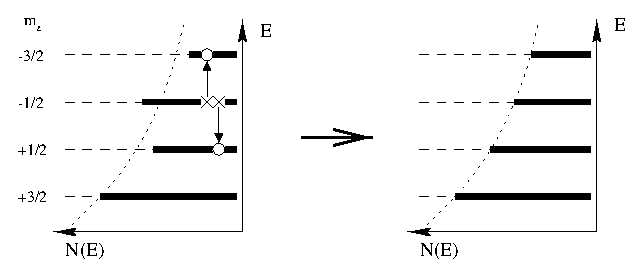
\includegraphics{drawings/relax_transition.eps}$$
	\caption[Skizze zur Einstellung des thermischen Gleichgewichts der
		Kernspins.]{{\upshape\bfseries Einstellung des thermischen Gleichgewichts der Kernspins.} Zwei
		Spins koppeln und gehen unter Erhaltung der Gesamtenergie und des Gesamtspins in einen
		jeweils anderen Zustand über.}
	\label{fig:relax_transition}
\end{figure}

Wie in Abbildung~\ref{fig:relax_transition} gezeigt koppeln die Spins ($\times$) im Niveau
$m=-\frac12$ und gehen in den Zustand ($\circ$) mit $m=-\frac32$ bzw.\ $m=\frac12$ über.
Für die Übergangsraten für diesen und den umgekehrten Prozeß gilt:
	\begin{equation}
		\left.\frac{dN}{dt}\right|_{\times\rightarrow\circ}=p_{-\frac12}p_{-\frac12}W_{\times\rightarrow\circ}\ttextt{und}
		\left.\frac{dN}{dt}\right|_{\circ\rightarrow\times}=p_{-\frac32}p_{\frac12}W_{\circ\rightarrow\times}
	\end{equation}
Im thermischen Gleichgewicht müssen diese beiden Übergangsraten übereinstimmen, da auch noch
$W_{\times\rightarrow\circ}=W_{\circ\rightarrow\times}$ gilt, erhält man:
	\begin{equation}
		\frac{p_{-\frac32}}{p_{-\frac12}}=\frac{p_{-\frac12}}{p_{+\frac12}}\quad.
	\end{equation}
Dies ist genau die Bedingung für ein thermisches Gleichgewicht nach Boltzmann, da sich die
Zustände um einen konstanten Energieabstand, also in ihrer Besetzung um einen konstanten Faktor
unterscheiden.

Man sieht, daß das thermische Gleichgewicht durch solche Prozesse erreicht wird. Die typische
Übergangsrate zwischen den Zuständen liegt in der Größenordnung der inversen Linienbreite, also bei
Metallen typischerweise in der Größenordnung von $10$ bis $100\;$µs. Falls $T_1$ viel größer als
diese Zeit zur Einstellung eines thermischen Gleichgewichts im Spinsystem ist, also z.\ B. in der
Größenordnung von Millisekunden bis Sekunden liegt, kann man die Besetzung der Kernspin"=Niveaus
als durch die Boltzmannverteilung für die Spintemperatur $T_S$ gegeben annehmen. Die Spintemperatur
stellt sich unter Erhaltung des Gesamtspins ein und kann für Tippingwinkel größer 90° aufgrund der
stärkeren Besetzung der höheren Energieniveaus auch negativ werden.

Das Spinsystem ist also durch eine Temperatur $T_S$ beschrieben, da die Besetzung der Zustände nach
\eqref{eqn:boltzmann} gegeben ist, obwohl es sich nicht im thermischen
Gleichgewicht mit einem Wärmereservoir befindet.

Die Spin"=Gitter"=Relaxation ist nun der Ausgleich des Temperaturunterschiedes zwischen der
Spintemperatur $T_S$ und der Temperatur des "`Gitters"'. Unter der Annahme, daß die
Kernspinniveaus immer einer Boltzmannverteilung genügen, kann man für die zeitliche Änderung der
inversen Spintemperatur $\beta_S=\frac1{k_BT_S}$ folgende Differentialgleichung herleiten \cite[S. 148ff]{Slichter}:
	\begin{equation}
		\frac{d\beta_S}{dt}=(\beta-\beta_S)\left[\frac12\frac{\sum_{m,n}W_{mn}(E_m-E_n)^2}{\sum_nE^2_n}\right]
			= \frac{\beta-\beta_S}{T_1}
	\end{equation}
\begin{description}
	\item[$\beta=\frac1{k_BT_\mathrm{el}}$] ist hier die inverse Temperatur des "`Gitters"'.
	\item[$W_{nm}$] stellt die Wahrscheinlichkeit für einen vom Gitter induzierten Übergang des
		Systems von Zustand $m$ in den Zustand $n$ dar.
\end{description}
Für die Relaxationszeit $T_1$ ergibt sich somit allgemein:
	\begin{equation}
		\label{eqn:t1}
		\frac1{T_1}=\frac12\frac{\sum_{m,n}W_{mn}(E_m-E_n)^2}{\sum_nE^2_n}
	\end{equation}

\subsection{Spin"=Gitter"=Relaxation der Kerne in einem Metall}

Der dominante Mechanismus der Spin"=Gitter"=Relaxation der Kerne in einem Metall ist die Kopplung an
die spin"=magnetischen Momente der Leitungselektronen.

In einem solchen $T_1$"=Prozeß gibt der Kern entweder Energie ab oder nimmt sie auf. Da die
Gesamtenergie von Gitter und Spinsystem erhalten bleibt, muß das Gitter (also das Wärmebad) dies
kompensieren. Die Kopplung an die Leitungselektronen kann man sich als einen gekoppelten Übergang
eines Kerns und eines Leitungselektrons mit Wellenvektor $\vec k$ und Spin"=Orientierung
$s$ zum Zustand $\vec k', s'$ als eine Art Streuprozeß vorstellen. Wenn man die Start"=
und Ziel"=Quantenzahlen mit $m$ und $n$ bezeichnet, erhält man für die Anzahl der Übergänge pro
Sekunde vom Startzustand $|m\vec ks>$ von Kern und Elektron zum Zielzustand $|n\vec k's'>$:
	\begin{equation}
		W_{m\vec ks, n\vec k's'}=
			\frac{2\pi}{\hbar}\abs{<m\vec ks|V|n\vec k's'>}^2\delta(E_m+E_{\vec ks}-E_n-E_{\vec k's'})
	\end{equation}
Wobei $V$ die Streu"=Wechselwirkung darstellt und angenommen wird, daß ein Elektron im Zustand
$|\vec ks>$ existiert und der Zustand $|\vec k's'>$ unbesetzt ist. Die Gesamtwahrscheinlichkeit
pro Sekunde für einen Übergang erhält man durch Summation über alle möglichen $W_{m\vec ks, n\vec
k's'}$
	\begin{equation}
		W_{mn}=\sum_{\vec k s \text{ besetzt}\atop\vec k's'\text{ unbesetzt}}W_{m\vec ks, n\vec k's'}\ttext{.}
	\end{equation}
Nun geht man zur Fermi"=Funktion $f(E_{\vec ks})$ als Verteilungsfunktion der Elektronen über und
setzt als Hauptbeitrag zur Streu"=Wechselwirkung $V$ die Kopplung der $s$"=Wellenfunktionen der
Elektronen an die Kerne an:
	\begin{equation}
		V=\frac{8\pi}{3}\gamma_e\gamma_n\;\hbar^2\vec I\cdot\vec S\,\delta(\vec r)
	\end{equation}
Hierbei nimmt man an, das sich der Kern am Ursprung des Koordinatensystems befindet und nur
Elektronen, die sich am Kernort befinden durch die Fermi"=Kontakt"=Wechselwirkung einen
Beitrag liefern.

Wenn man für die Wellenfunktion der Elektronen im Gitter das Produkt einer Spin"=Funktion und einer
Bloch"=Funktion $u_{\vec k}(\vec r)e^{i\vec k\cdot\vec r}$ ansetzt, kann man die Matrixelemente der
Streu"=Wechselwirkung berechnen. Die Summation über die Elektronenzustände kann man mit Hilfe der
Zustandsdichte $g(E_{\vec k})$ zu einer Integration über die Energie umformen. Zum Schluß ist noch
die Tatsache wichtig, daß nur Elektronen nahe der Fermi"=Kante an solchen Streuprozessen beteiligt
sein können, da die Energie, die zwischen Kern und Elektron ausgetauscht wird, im Falle hoher
Temperaturen viel kleiner als $k_BT$ ist und nur in der Nähe der Fermi"=Kante freie Zustände in
diesem Energieabstand erreicht werden können. Da die Anzahl der Elektronen in der Nähe der
Fermikante proportional zu $k_BT$ ist, folgt diese Proportionalität auch für $W_{mn}$.

Wenn man nun das berechnete $W_{mn}$ in die Gleichung \eqref{eqn:t1} einsetzt und noch über die
Anzahl $N$ der Kerne im Gitter summiert, erhält man die Korringa"=Relation \cite{Korringa}:
\begin{equation}
	\label{eqn:korringa}
	T_1\left(\frac{\Delta H}{H}\right)^2=\frac{\hbar}{4\pi k_BT_\mathrm{el}}\frac{\gamma_e^2}{\gamma_n^2}
\end{equation}
Wobei der Term $\frac{\Delta H}{H}$ die Größe der im folgenden Abschnitt erklärten Knightshift
nach \eqref{eqn:knightshift} darstellt. Die Korringarelation bestimmt das Verhältnis
von Spin"=Gitter Relaxationzeit $T_1$ , Knightshift $\frac{\Delta H}{H}$ und der
Elektronentemperatur $T_\mathrm{el}$.

%%%%%%%%%%%%%%%%%%%%%%%%%%%%%%%%%%%%%%%%%%%%%%%%%%%%%%%%%%%%%%%%%%%%%%%%%%%%%%%%%%%%%%%%%%%%%%%%%%

\section{Frequenzverschiebung in Metallen --- Knightshift}
Entdeckt wurde die Knightshift aufgrund der Verschiebung der Resonanzfrequenz in $^{63}$Cu. Da
diese Verschiebung mit 0.23\% höher ist als bekannte chemische Verschiebungen verschiedener
diamagnetischer Komponenten, suchte man den zugrundeliegenden Effekt im Metall. Darauffolgende
Untersuchungen zeigten, das dieses Phänomen in allen Metallen auftritt. Wenn man
$\omega_\mathrm{M}$ für die Resonanzfrequenz und $\omega_\mathrm{D}$ für die Resonanzfrequenz in
einer diamagnetischen Referenzumgebung schreibt, ist die Frequenzverschiebung $\Delta\omega$ bei dem
selben statischen Magnetfeld durch $\omega_\mathrm{M} = \omega_\mathrm{D} + \Delta\omega$
mit folgenden Eigenschaften gegeben:
	\begin{enumerate}
		\item $\Delta\omega$ ist im Allgemeinen positiv.
		\item Die relative Verschiebung $\frac{\Delta\omega}{\omega_\mathrm{D}}$ bleibt bei
			veränderlicher Stärke des stationären Magnetfeldes konstant.
		\item Die relative Verschiebung $\frac{\Delta\omega}{\omega_\mathrm{D}}$ ist annähernd
			temperaturunabhängig.
		\item Die relative Verschiebung nimmt im Allgemeinen mit steigender Kernladungszahl $Z$
			ab.
	\end{enumerate}

Diese zusätzliche Verschiebung der Resonanzfrequenz in Metallen folgt analog zur
Spin"=Gitter"=Relaxation aus der Kopplung der Elektronenwellenfunktionen mit $s$"=Charakter an die
Kernspins. Die Polarisation der Elektronen hängt nur vom äußeren Magnetfeld $B_0$ ab, da der
Spin"=Paramagnetismus des stark entarteten Elektronengases der Leitungselektronen unabhängig von
der Temperatur ist. Die Verschiebung $\Delta\omega$ ist also temperaturunabhängig. Die
Abhängigkeit der Verschiebung von der Kernladungszahl ist durch die bekannte, mit steigendem $Z$
größer werdende Hyperfeinaufspaltung freier Atome erklärt.

Diese Kopplung hat in Metallen, obwohl sie durch den gleichen Hamiltonian wie in Nichtmetallen
beschrieben wird, einige Besonderheiten, die aus folgenden Eigenschaften der Leitungselektronen
herrühren:

 \begin{enumerate}
	\item Die Leitungselektronen sind nicht lokalisiert. Ein bestimmtes Leitungselektron, daß nach
		dem Bloch"=Theorem durch die Wellenfunktion $\phi_{\vec k}(\vec r)=u_{\vec k}(\vec
		r)e^{i\vec k\cdot\vec r}$ beschrieben ist (mit $u_{\vec k}(\vec r)$ periodisch im
		Kristallgitter und im Volumen $V$ der Probe normiert), besitzt in der Nähe jedes Kernspins
		im Gitter die gleiche Aufenthaltswahrscheinlichkeit. Analog sieht jeder Kernspin
		gleichzeitig die Magnetfelder aller Leitungselektronen des Metalls.
	\item Für die Größenordnung der Elektronendichten $N$, die in Metallen vorkommen, verhalten
		sich die Leitungselektronen sogar bei Raumtemperatur wie ein entartetes Fermi"=Gas. In
		Anwesenheit eines Magnetfeldes $H$ sind alle Energieniveaus, außer denen in der Nähe
		der Fermi"=Energie, mit zwei Elektronen entgegengesetzten Spins aufgefüllt. Die paramagnetische Suszeptibilität
		der Leitungselektronen $\chi_e^s$ ist deshalb im Gegensatz zu der der gebundenen
		Elektronen nahezu temperaturunabhängig.
 \end{enumerate}

Wenn man zur Vereinfachung annimmt, daß das Bahnmoment der Elektronen komplett ausgelöscht ist,
erhält man die Kopplung eines gegebenen Kernspins $I$ mit den Elektronen durch Summation der
Erwartungswerte der Hyperfeinkopplungen dieses Kernspins mit allen Leitungselektronen.

Der Kernspin $\vec I$ sieht ein internes Feld $\Delta H$, das das angelegte Feld $H_0$
überlagert und eine paramagnetische Verschiebung der Kernresonanz verursacht, die als
Knightshift\footnote{nach W. D. Knight, der diese Verschiebung 1949 als erster beobachtete}
bekannt ist \cite{KNIGHT49}.
	\begin{equation}
		\label{eqn:knightshift}
		\frac{\Delta H}{H_0}=\frac{8\pi}{3}\left<\abs{u_{\vec k}(0)}^2\right>_{E_F}\chi_e^s
	\end{equation}

\chapter{NMR"=Messungen an \aug}
\section{Herstellung und Charakterisierung der \aug"=Probe}

Die Kristallstruktur des \aug{} entspricht dem CaF$_2$"=Gitter und ist in Abbildung~\ref{fig:auga2}
dargestellt. Die Galliumatome besetzen darin ein einfach kubisches Untergitter. Deswegen ist die
bei reinem Gallium mit seiner orthorhombischen Struktur auftretende starke Quadrupolaufspaltung bei
Gallium in \aug{} unterdrückt.

\begin{figure}[htp]
	$$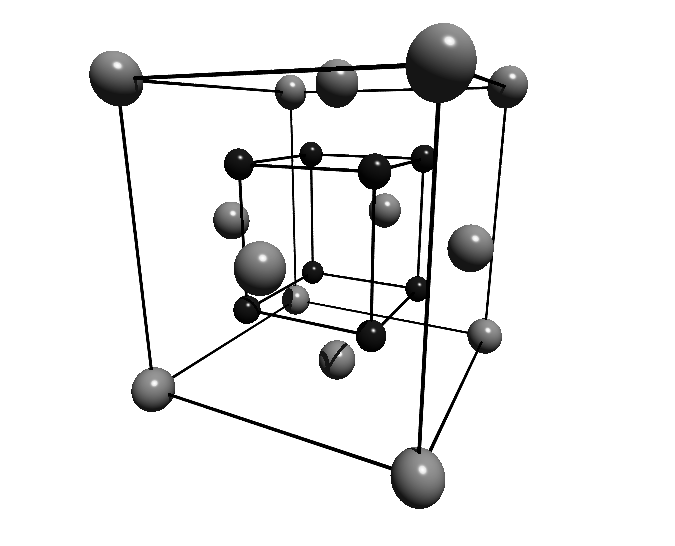
\includegraphics{drawings/auga2}$$
	\caption[Das Kristallgitter von AuGa$_2$]{{\upshape\bfseries Das Kristallgitter von \aug.} Die kleineren Galliumatome bilden im
		kubisch flächenzentrierten Gitter der Goldatome ein einfach kubisches Untergitter. Die
		Gitterkonstante beträgt 6.075Å und in einer Elementarzelle befinden sich 8 Gallium"= und 4
		Goldatome}
	\label{fig:auga2}
\end{figure}

\newcommand{\khzpmt}{\ensuremath{\left[\frac{\mathrm{kHz}}{\mathrm{mT}}\right]}}
{\setlength{\tabcolsep}{0.2em}
\begin{table}
	$$\begin{tabular}{|c||c|c|c|c|c|c|c|c|}
		\hline
		Isotop		& $\gamma$	& $\K$	& $\gamma(1+\K)$	& $I$	& Häufigkeit	& $\mu$ &$T_\mathrm{el}T_1$	& $T_2$\\
					& \khzpmt	& [\%]		& \khzpmt		&		& [\%]			&[$\mu_N$]		&[Ks]	& [$µ$s]\\\hline\hline
		$^{63}$Cu	& 11.285	& 0.238		& 11.312		& 3/2	& 69.17			& 2.2206	& 1.27	& 150\\
		$^{65}$Cu	& 12.089	& 0.238		& 12.118		& 3/2	& 30.83			& 2.3791	& 1.09	& 150\\\hline
		\ga			& 10.219	& 0.132		& 10.232		& 3/2	& 60.1			& 2.0108	& 1.008	& 320\\
		\gb			& 12.984	& 0.132		& 13.001		& 3/2	& 39.9			& 2.5549	& 0.630	& 260\\\hline
		$^{197}$Au	& 0.72919	& 1.65		& 0.7412		& 3/2	& 100			& 0.14349 	& 4.6	& ---\\\hline
	\end{tabular}$$
	\caption[NMR"=spezifische Parameter der reinen Metalle]{{\upshape\bfseries NMR"=spezifische
			Parameter der reinen Metalle Kupfer, Gallium und Gold.} Werte entnommen aus \cite{Metallic,Valic}}
\end{table}}

Die Atommassen der reinen Komponenten Gallium und Gold sind $m_\mathrm{Ga}=69.723$u und
$m_\mathrm{Au}=196.967$u. Daraus ergibt sich für die Dichte von \aug{}:
	\begin{equation}
		\rho_\aug=
			\frac{8m_\mathrm{Ga}+4m_\mathrm{Au}}{6.022\cdot10^{26}\frac{\mathrm{u}}{\mathrm{kg}}}
				\frac1{\left(6.075\cdot10^{-10}\mathrm{m}\right)^3}
			= 9966.7 \frac{\mathrm{kg}}{\mathrm{m}^3}
	\end{equation}
Die Gewichtsanteile der Bestandteile Gold und Gallium an der Verbindung
\aug{} bestimmt man aus den Atommassen zu 41.451\% Gallium und 58.549\% Gold.

Das Gefäß zum Einschmelzen der Ausgangselemente besteht aus einer an ein Quarzglasrohr mit 9 mm
Innendurchmesser angeschmolzenen 2 cm langen Quarzglaskapillare mit einem Innendurchmesser von 3
mm. Damit diese Kapillare, die später als Form für die Gold"=Gallium"=Schmelze dient, vollständig
mit \aug{} gefüllt werden kann, sind ungefähr 2 g davon nötig. Es wurde nun die entsprechende Menge
von 1.1805 g 5N$^+$ Gold und 0.8350 g 6N$^+$ Gallium (Sollwert nach den stöchiometrischen Gewichtsanteilen:
0.8357 g) zusammen in das Quarzglasrohr eingebracht, welches anschließend mit einer
Drehschieberpumpe evakuiert und zugeschmolzen wurde. Nun wurden die Komponenten im liegenden
Quarzglasrohr 22 Stunden lang bei 550°C eingeschmolzen. Der Schmelzpunkt von \aug{} liegt bei etwa
496°C. Obwohl der Schmelzpunkt von Gold bei 1064°C liegt, löst es sich bei einer Temperatur von
550°C im bereits bei 30°C schmelzenden Gallium. Danach wurde das flüssige Gold"=Gallium"=Gemisch
durch Aufstellen des Quarzglasrohres in die als Probenform dienende Quarzglaskapillare eingefüllt
und zuerst in 24 Stunden auf 360°C, dann in 38 Stunden auf 120°C und schließlich bis zur
Raumtemperatur abgekühlt.

\subsection{Das Restwiderstandsverhältnis}

Das Restwiderstandsverhältnis (\ul{r}esidual \ul{r}esistivity \ul{r}atio, RRR) läßt Rückschlüsse auf die
Stärke der Streuung von Elektronen an Verunreinigungen und Gitterdefekten bei tiefen Temperaturen
zu. Bei der Streuung an Verunreinigungen muß man folgende Fälle unterscheiden:

\begin{figure}[htp]
	\begin{center}
		\subfigure[bei Raumtemperatur / in flüssigem N$_2$]{
			$$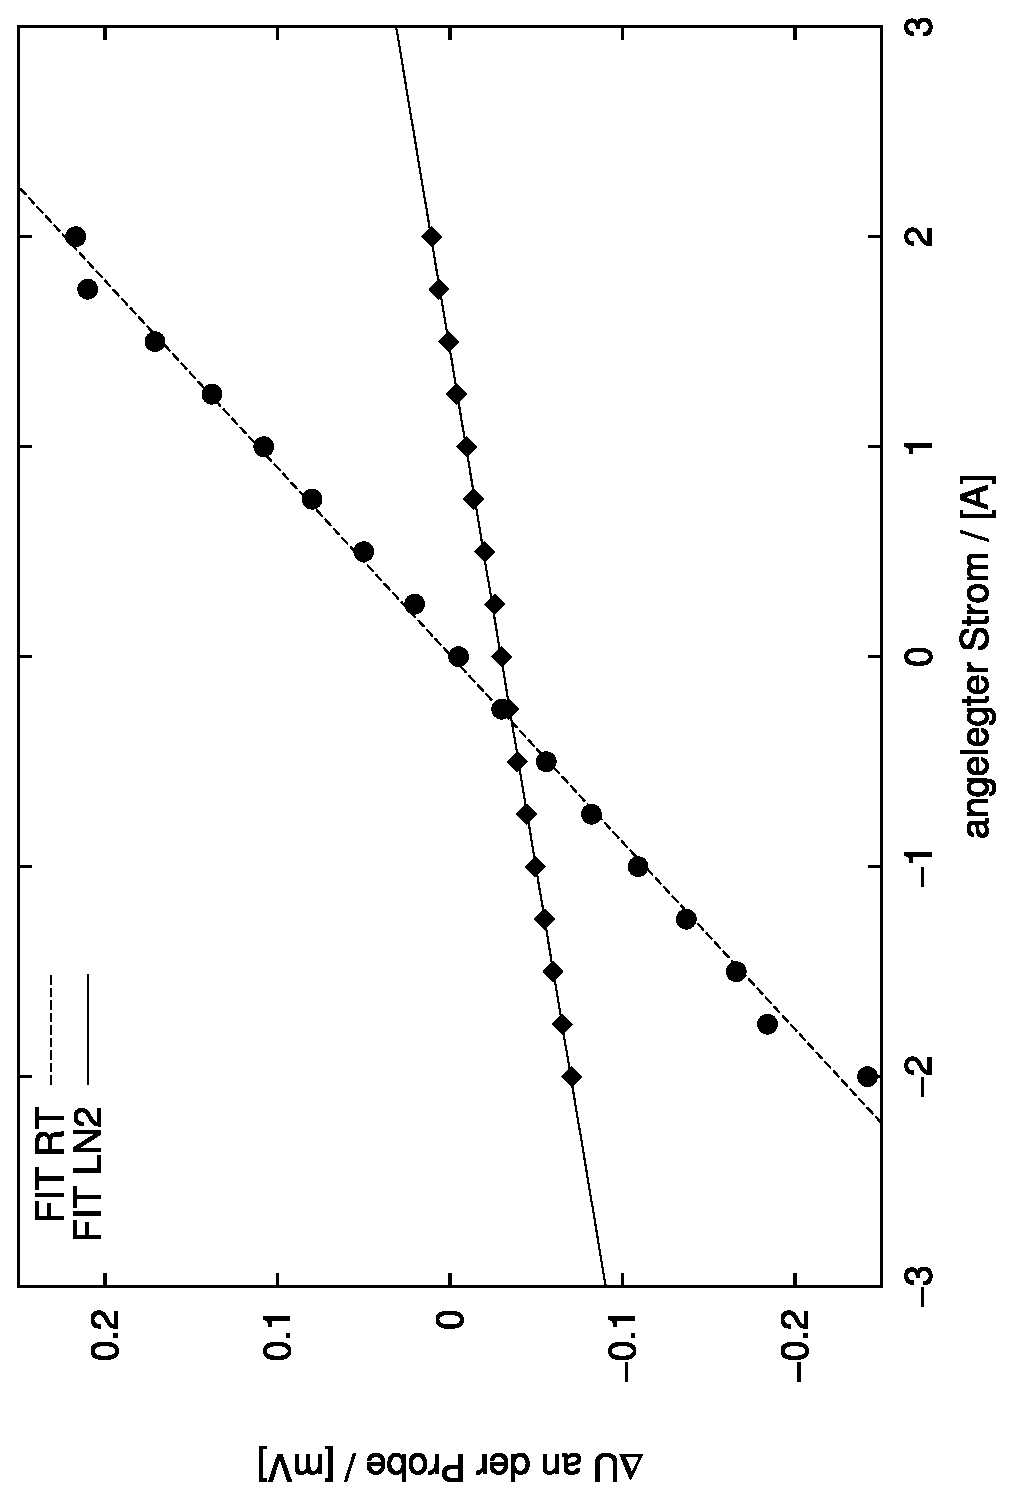
\includegraphics[angle=-90,width=\bigwidth]{plots/rrr1}$$}
		\hspace{1em}
		\subfigure[in flüssigem $^4$He]{
			\label{fig:rrr2}
			$$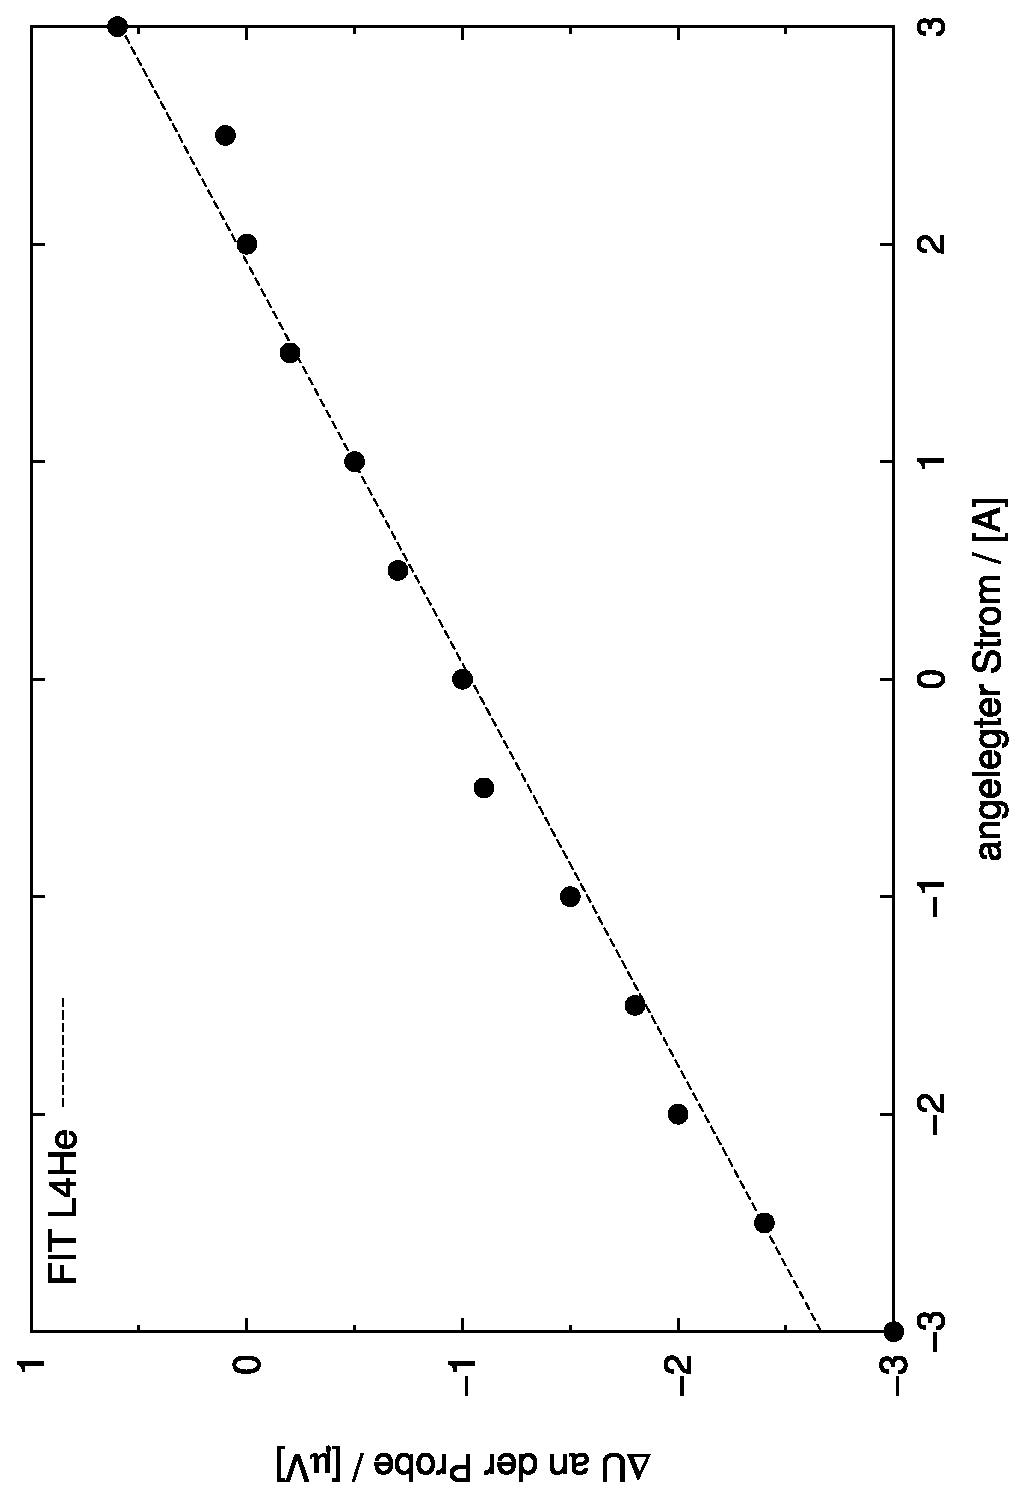
\includegraphics[angle=-90,width=\bigwidth]{plots/rrr2}$$}
		\caption[Messung des Restwiderstandsverhältnisses]{{\upshape\bfseries Messung des Restwiderstandsverhältnisses der \aug"=Probe}
			mit Hilfe der 4"=Punkt Methode. Aufgetragen ist der gemessene Spannungsabfall an der
			Probe über den durch die Probe fließenden Strom. Der auftretende Spannungsoffset bei
			der Messung kommt durch auftretende Thermospannungen zustande. Dies hat jedoch keinen
			Einfluß auf das Meßergebnis, da die Steigung der Geraden $U(I)=R\cdot I$ ausgewertet
			wird.}
		\label{fig:rrr}
	\end{center}
\end{figure}

\begin{description}
	\item[die Streuung an nichtmagnetischen Verunreinigungen:] Die Leitungselektronen werden durch
		das Coulombpotential der Verunreinigung gestreut, sie sehen den Unterschied $\Delta$Z der
		Kernladungszahl des Verunreinigungsatoms. Die Vergrößerung des Widerstandes ist
		nicht sehr groß und für kleine Konzentrationen der Verunreinigung gilt das Gesetz von
		Linde:
		\begin{equation}
			\Delta\rho = a + b(\Delta\mathrm{Z})^2
		\end{equation}
		Wobei die Konstanten $a$ und $b$ vom jeweiligen Hauptbestandteil des Metalls abhängen.

	\item[die Streuung an magnetischen Verunreinigungen:] Eine Streuung mit Spinübergängen kann an
		den lokalisierten Momenten der Verunreinigungsatome erfolgen. Hierbei ist die Erhöhung
		des Widerstandes in der Regel wesentlich stärker als im Fall von nichtmagnetischen
		Verunreinigungen. Die Stärke der Streuung und die daraus resultierende Erhöhung des
		Widerstandes ist stark von den Eigenschaften der Verunreinigungsatome und des
		Gastgitters abhängig. Sie kann aufgrund des auftretenden
		Kondo"=Effektes\footnote{eine verstärkte inelastische Streuung einer Wolke von
		Leitungselektronen in der Nähe eines Verunreinigungsatomes mit magnetischen Moment,
		welches dadurch von den Leitungselektronen temperaturabhängig nach außen abgeschirmt wird}
		eine starke Temperaturabhängigkeit besitzen.
\end{description}

Für die Widerstände der \aug"=Probe ergeben sich aus der Messung in Abbildung~\ref{fig:rrr} folgende Werte
	$$\begin{tabular}{|r|c|}\hline
		T / [K]	& R / [m$\Omega$]\\\hline\hline
		300 K	& $112.2\pm1.4$\\
		77	K	& $20.25\pm0.12$\\
		4.2 K	& $0.5418\pm0.020$\\\hline
	\end{tabular}$$
Daraus folgt für das Restwiderstandsverhältnis der untersuchten Probe:
	\begin{equation}
		\mathrm{RRR}=\frac{R_\mathrm{300K}}{R_\mathrm{4.2K}}
			=\frac{112.2\pm1.4\,\mathrm{m}\Omega}{0.5418\pm0.020\,\mathrm{m}\Omega}=207.1\pm8.1
	\end{equation}

\subsection{Die statische Suszeptibilität}

Die Messung des magnetischen Moments der \aug"=Probe im Temperaturbereich 4.2~K $\le$ T $\le $300~K
im statischen Feld B=0.5~T dient zur Untersuchung der elektronischen magnetischen Eigenschaften
sowie der magnetischen Verunreinigungen der Probe.

 \begin{figure}[htp]
	\begin{center}
		\subfigure[Der Verlauf der statischen Suszeptibilität im gemessenen Temperaturbereich]{
			\label{fig:suszept}
			$$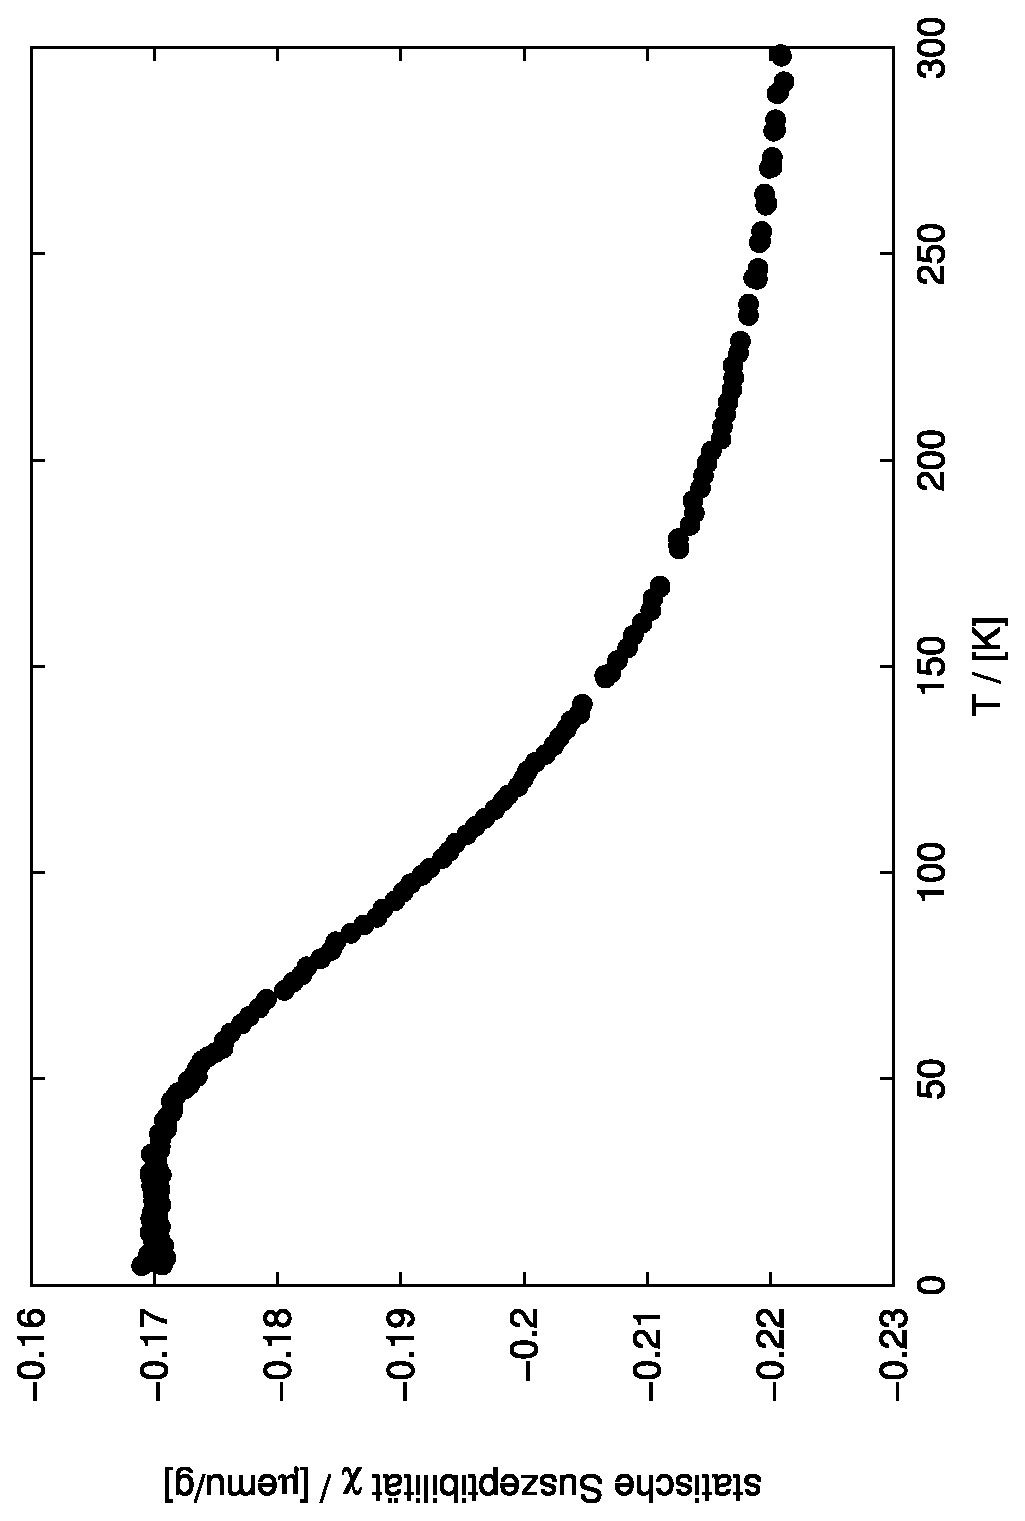
\includegraphics[angle=-90,width=\bigwidth]{plots/suszept1}$$}\\
		\subfigure[magn. Moment nach Abzug des diamagnetischen Anteils bei tiefen Temperaturen]{
			\label{fig:suszept2}
			$$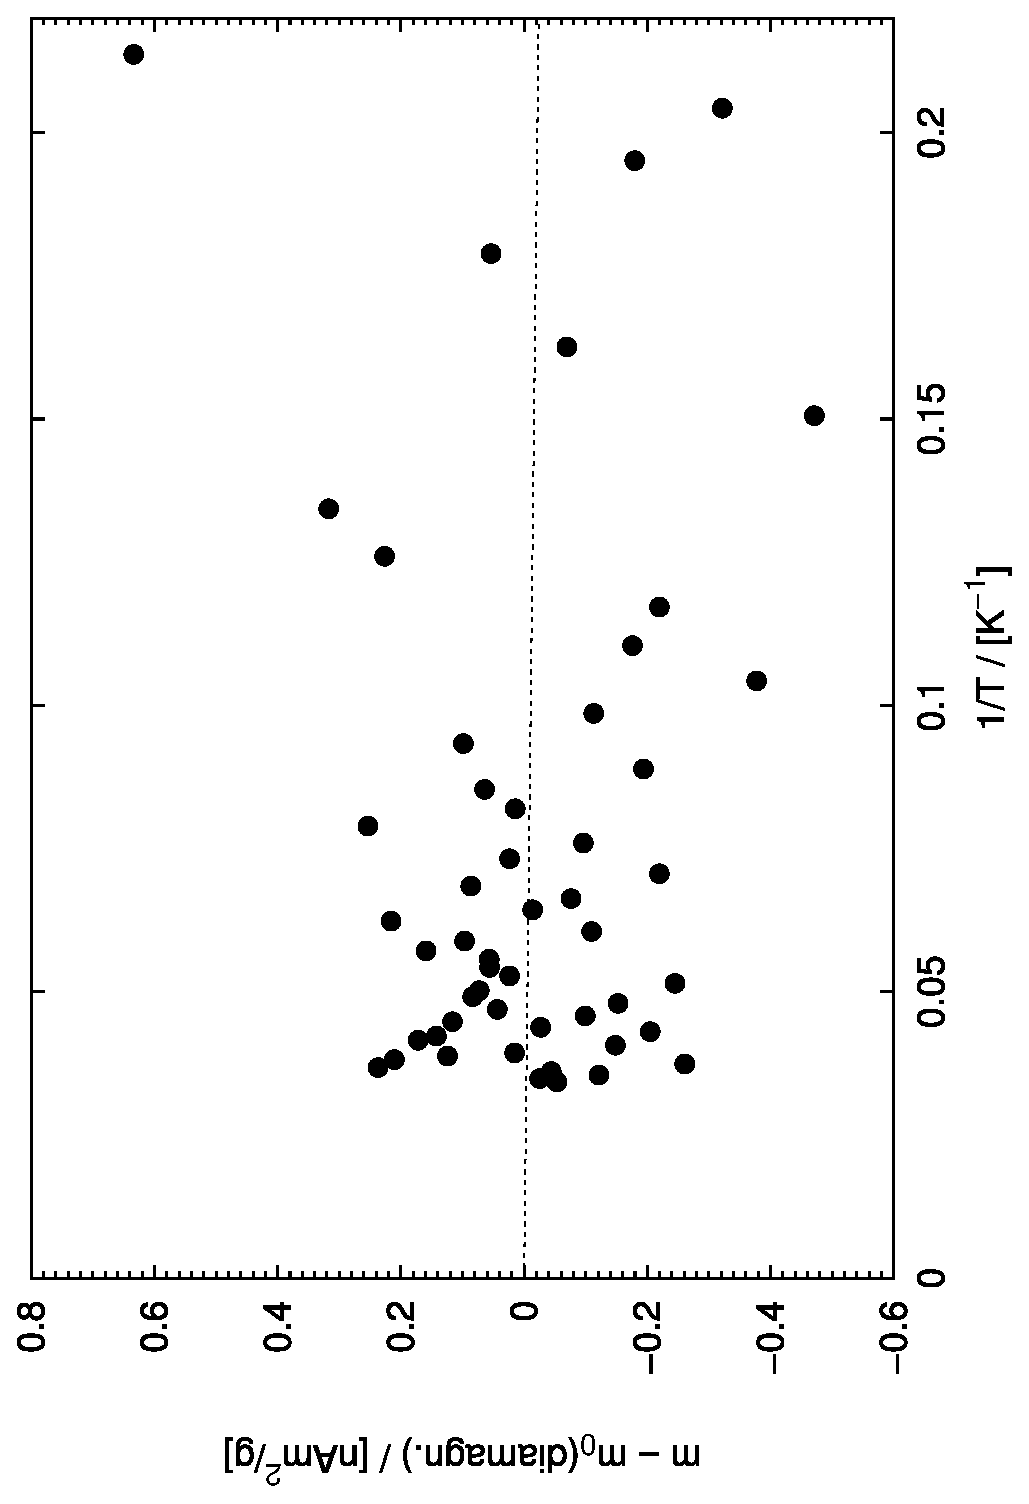
\includegraphics[angle=-90,width=\bigwidth]{plots/suszept2}$$}
	\caption[Messung der statischen Suszeptibilität]{{\upshape\bfseries Messung der statischen Suszeptibilität von \aug{}} bei einem
		Magnetfeld $B=0.5$T im Temperaturbereich von 300 K bis 4.2K. Die Gerade
		$f(x)=(-0.1\pm0.6)\frac1{T}$ repräsentiert die Anpassung der Tieftemperaturdaten an das
		Curie"=Gesetz, zur Bestimmung der Größenordnung der magnetischen Verunreinigungen in der Probe}
	\end{center}
 \end{figure}

Diese Messung wurde mit einem kommerziellen SQUID"=Magnetometer an einem zylindrischen Teil der
gewonnenen \aug"=Probe der Masse 0.3041~g im Temperaturbereich von 4.2~K bis zur Raumtemperatur bei
einem statischen Magnetfeld $B=0.5$~T durchgeführt.

Aus der gemessenen Magnetisierung kann man die Konzentration $x_\mathrm{mag}$, das effektive Moment
$N_\mathrm{eff}$ sowie die Spinquantenzahl $S$ von verdünnten also von nur schwach
wechselwirkenden magnetischen Verunreinigungen bestimmen.

Die Magnetisierung eines Systems elektronischer magnetischer Momente läßt sich durch die
Brillouinfunktion \eqref{eqn:brillouin} beschreiben:
	\begin{equation}
		\label{eqn:suszept}
		M = \frac{x_\mathrm{mag}N_0\mu}{V_\mathrm{mol}}B_s(x)\ttextt{mit}
			x=\frac{\mu\,B}{k_B\,T}\ttextt{und}\mu=\mu_Bg_eS
	\end{equation} 
Für $x\gg1$ sättigt die Magnetisierung und $M$ geht gegen $M_\mathrm{sat}$. Das effektive magnetische Moment
ist dabei $N_\mathrm{eff}\mu_B=g_e\sqrt{S(S+1)}\mu_B$. Aus der gemessenen Magnetisierungskurve
$M(T,B)$ können $x_\mathrm{mag}$, $N_\mathrm{eff}(g_e,S)$ und $S$ mit Hilfe von \eqref{eqn:suszept}
unabhängig voneinander bestimmt werden, wenn die Magnetisierung sättigt.


Um nun die Konzentration kernmagnetischer Verunreinigungen zu bestimmen, subtrahiert man von der
gemessenen Suszeptibilität den diamagnetischen Anteil der Elektronen, der in
Abbildung~\ref{fig:suszept} mit seinem, durch die Brillouinfunktion gegebenen Verlauf dominiert.
Nun betrachtet man den Verlauf der Suszeptibilität bei tiefen Temperaturen.

Da man sich für T > 4.2~K nur im Gültigkeitsbereich des Curie"=Gesetzes für kernmagnetische Verunreinigungen
befindet, ist es nicht möglich, die Daten aus Abbildung~\ref{fig:suszept2} an
Gleichung~\eqref{eqn:suszept} anzupassen. Aus einer Anpassung an das Curie"=Gesetz, für das sich bei
Auftragung über $1/T$ in Abbildung~\ref{fig:suszept2} eine Gerade ergibt, erhält man nach
	\begin{equation}
		\label{eqn:suszept2}
		M = \frac{C}{\mu_0V_\mathrm{mol}}\frac{B}{T} \ttextt{mit}
			C=\frac{x_\mathrm{mag}N_0\mu_0\mu_B^2g_e^2S(S+1)}{3k_B}
	\end{equation}
nur den Faktor $x_\mathrm{mag}\cdot N_\mathrm{eff}^2$. Allerdings muß man, um $x_\mathrm{mag}$
daraus bestimmen zu können, einen plausiblen Wert für das effektive magnetische Moment der
Verunreinigungsatome $N_\mathrm{eff}$ annehmen.

Für die Messung an der \aug"=Probe ergibt sich für $N_\mathrm{eff}=5$ (nach \cite{Doofi}) eine Obergrenze
für die magnetischen Verunreinigungen von $x_\mathrm{mag}< 1$~ppm. Dies stellt bei einem
Feld von 0.5 T die Auflösungsgrenze des verwendeten Suszeptometers dar. 

%%%%%%%%%%%%%%%%%%%%%%%%%%%%%%%%%%%%%%%%%%%%%%%%%%%%%%%%%%%%%%%%%%%%%%%%%%%%%%%%%%%%%%%%%%%%%%%%%%

\section{Der Versuchsaufbau}

\subsection{Der Kryostat}
 \begin{figure}[htp]
	$$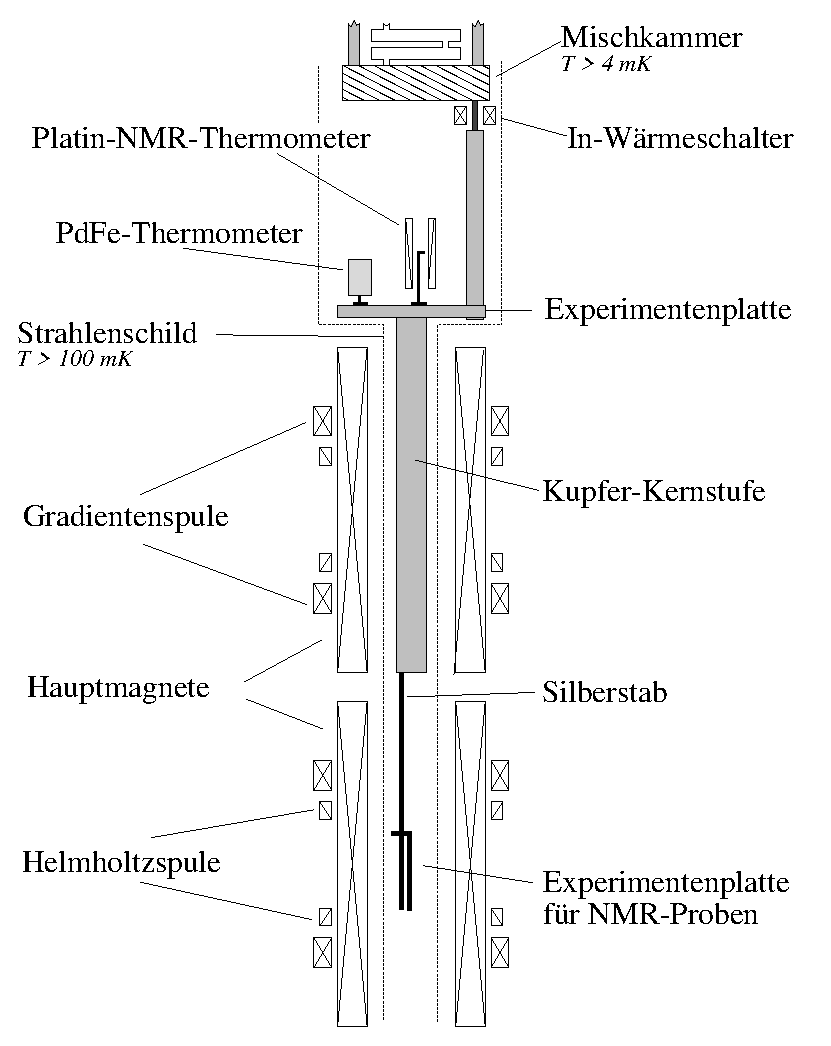
\includegraphics[width=0.6\textwidth]{drawings/kryo}$$
	\caption[Schematische Darstellung des Kryostaten WODAN]{{\bfseries\upshape Schematische Darstellung des Kryostaten WODAN}. Gezeigt sind nur die
		Bereiche, die auf Mischkammertemperatur ($T > 4$~mK) und tiefer
		($T_\mathrm{minimal}\approx0.2$~mK) abgekühlt werden. Zusätzlich ist noch das
		für die Kühlung durch adiabatische Entmagnetisierung und die NMR"=Experimente wichtige
		Magnetsystem abgebildet, das sich im Heliumbad des Kryostaten befindet.}
	\label{fig:Kryostat}
 \end{figure}

Die Messungen in der vorliegenden Arbeit wurden mit gepulster NMR am Kryostaten "`WODAN"' 
durchgeführt (siehe Abbildung~\ref{fig:Kryostat}). Die Basis des Kryostaten bildet ein
$^3$He"=$^4$He"=Entmischungskühler der Firma \emph{Oxford Instruments GmbH}, der um eine,
mittels supraleitenden Indium"=Wärmeschaltern abkoppelbare
Kupfer"=Entmagnetisierungsstufe mit Experimentenplatte und NMR Hochfeldmeßplatz
erweitert wurde. Eine genaue Beschreibung von Aufbau und Funktion des Kryostaten befindet sich in
der Dissertation von Thomas Wagner \cite{Wagner_Dis}.

\subsection{Das Puls"=NMR"=Spektrometer}
 \begin{figure}[htp]
	$$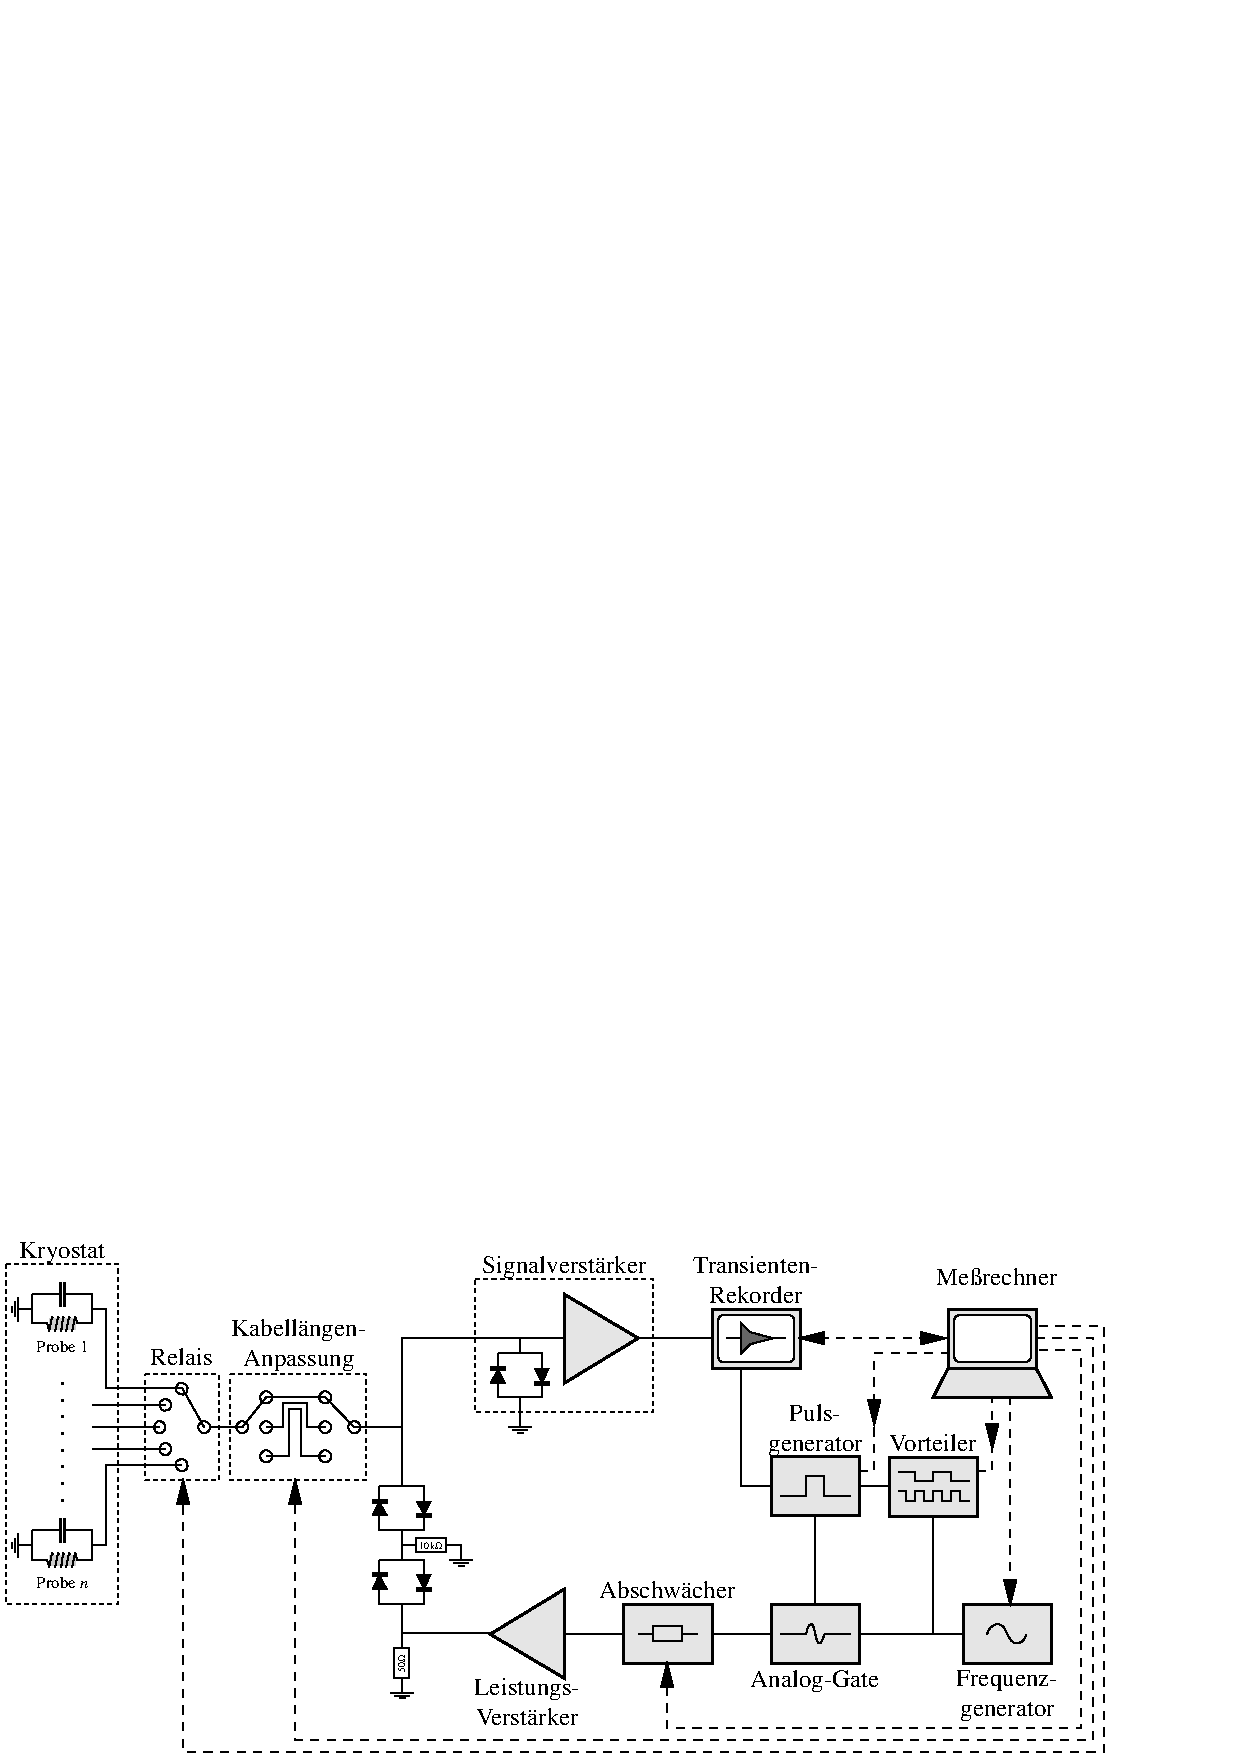
\includegraphics[bb=0 0 536 250,width=0.9\textwidth]{drawings/NMR-Setup}$$
	\caption[Schematischer Aufbau des Puls"=NMR"=Spektrometers]{{\upshape\bfseries Schematischer Aufbau des Puls"=NMR"=Spektrometers.}}
	\label{fig:NMR-Spektrometer}
 \end{figure}

Das für die Messungen verwendete NMR"=Spektrometer (Aufbauschema in
Abbildung~\ref{fig:NMR-Spektrometer}) ist aus Gründen der Flexibilität aus Einzelkomponenten
zusammengestellt und besitzt folgende Eigenschaften:
	\begin{itemize}
		\item Der mögliche Frequenzbereich erstreckt sich von 100 kHz bis zu 200 MHz.
		\item Es können aufeinanderfolgende Pulse mit \emph{starrer Phase} aufgenommen werden, was die
			Mittelung über mehrere aufgenommene FIDs zur Verbesserung des
			Signal"=Rausch"=Verhältnisses ermöglicht.
		\item Die verwendeten Analog"=Gates besitzen eine \emph{hohe Sperrdämpfung} von über 90 dB.
			Zusammen mit den antiparallelen Diodenpärchen nach dem Leistungsverstärker wird so
			gewährleistet, daß nur der verstärkte Puls und kein Rauschen oder
			Rest"=Hochfrequenzschwingung zur Probenspule gelangt.
		\item Zur Signaldetektion können wahlweise \emph{breitbandige} oder auf die zu verstärkende
			Frequenz \emph{abstimmbare Signalverstärker} mit kurzer Totzeit (typisch $\approx 5µ$s)
			verwendet werden.
		\item Eine weitere Verbesserung des Signal"=Rausch"=Verhältnisses erhält man durch
			Anpassung der Kabellängen nach \cite[S. 25f]{Micha_Dis} an die verwendete Pulsfrequenz.
	\end{itemize}
Eine ausführliche Beschreibung des verwendeten Spektrometers befindet sich in \cite{Wagner_Dis} und
\cite{Sigi_Dis}.

\subsubsection{Thermometrie}
Zur Thermometrie im Temperaturbereich von 0.2~mK bis zu 100~mK stehen zwei Thermometer zur
Verfügung. Zum einen ein \emph{Palladium"=Eisen Suszeptibilitätsthermometer}, das den
Temperaturbereich von 8 mK bis 100 mK abdeckt. Mit Hilfe dieses
PdFe"=Suszeptibilitätsthermometers ist es möglich, die Temperatur der
Experimentenplatte über einen Temperaturregler mit angeschlossenem Heizwiderstand zu
stabilisieren. Für Messungen von Temperaturen ab 100 mK bis herunter zu dem mit dem Kryostaten
minimal erreichbaren Wert von 0.2~mK wurde das \emph{Platin"=NMR"=Thermometer} verwendet. Da
beide Thermometer keine absoluten Thermometer sind, ist eine Eichung auf die supraleitenden
Übergänge eines Wolfram"=Fixedpointdevices bei 17 mK und 62 mK möglich.

\subsection{Die NMR"=Probe}
 \begin{figure}[htp]
	$$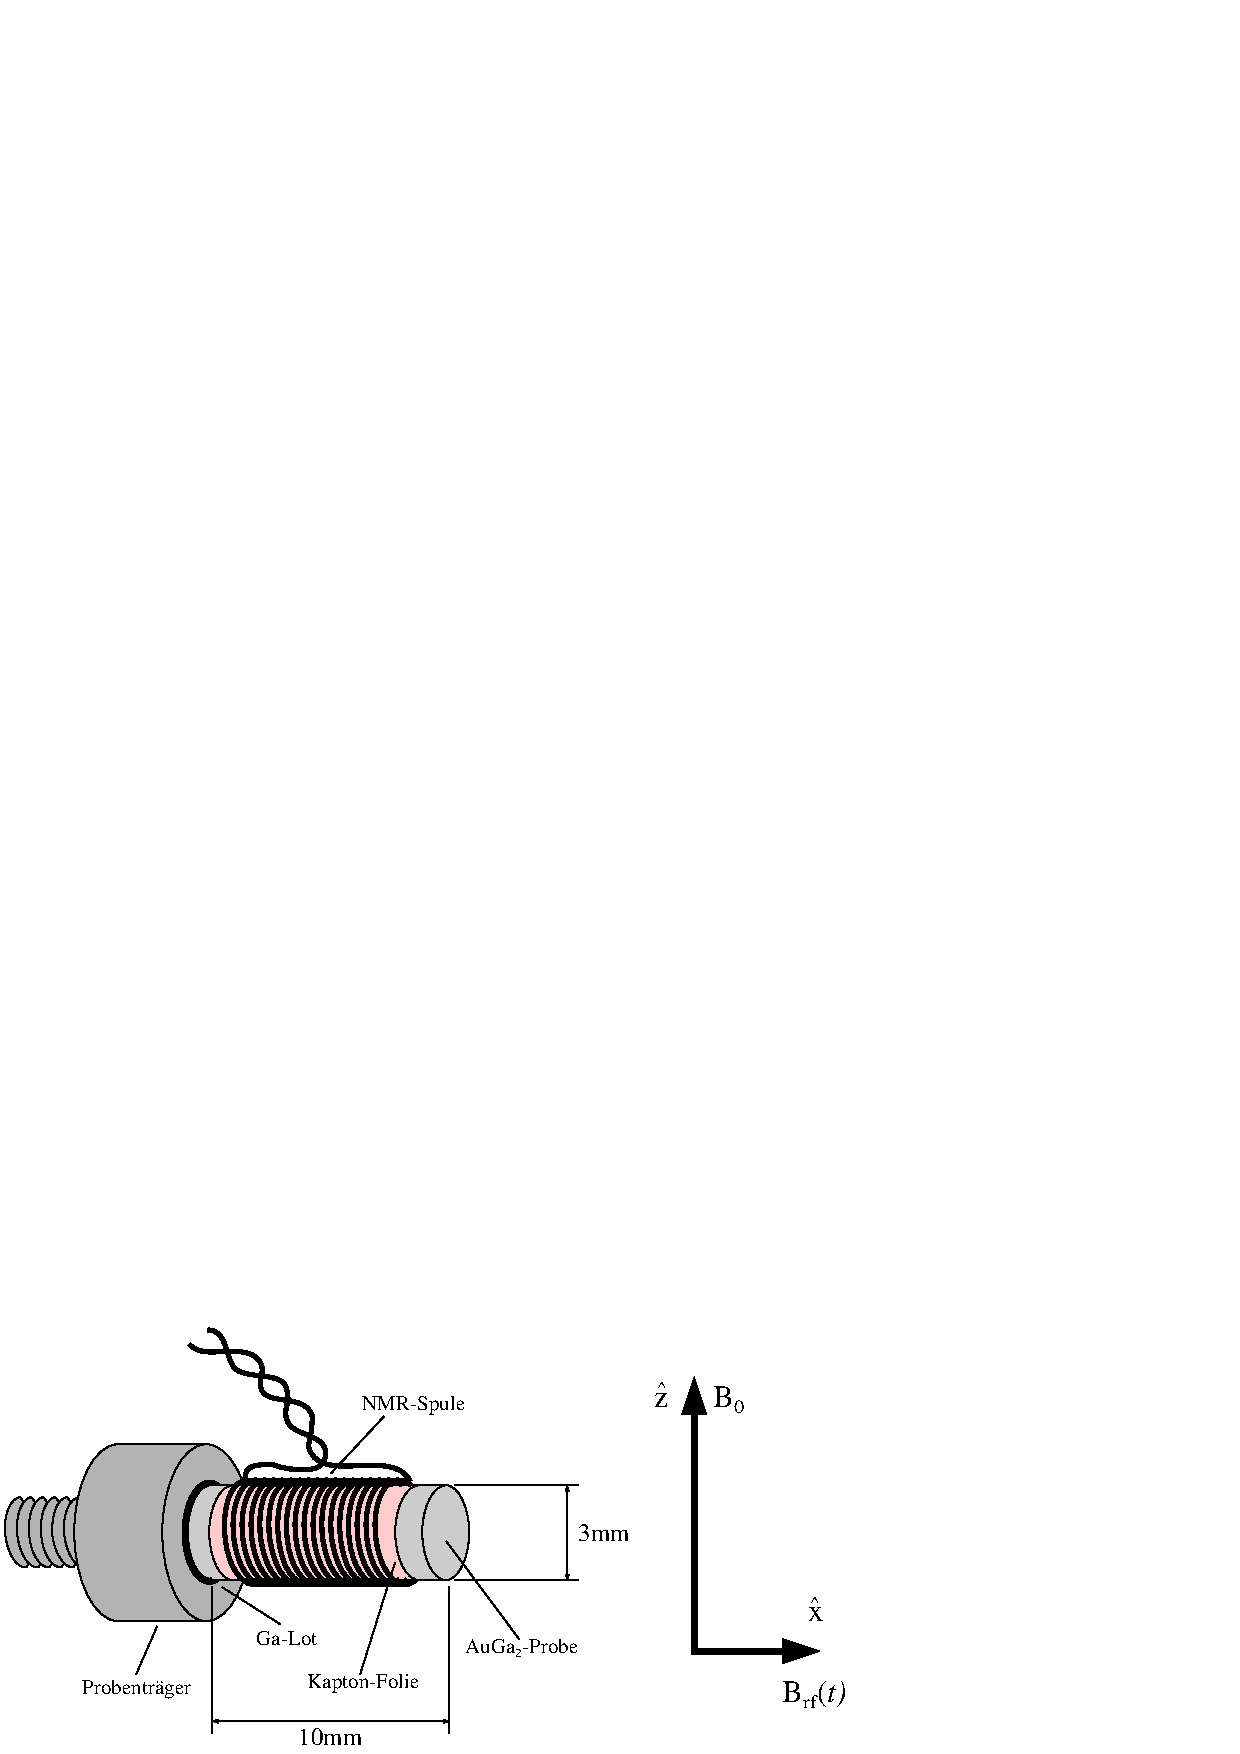
\includegraphics[bb=0 0 408 208]{drawings/probe}$$
	\caption[Skizze der AuGa$_2$ NMR"=Probe]{{\upshape\bfseries Die \aug{} NMR"=Probe.} Der Probenhalter wird mit dem M3"=Gewinde
		in die NMR"=Experimentenplatte im Hochfeldbereich des unteren Hauptmagneten eingeschraubt.
		Die Anschlüsse der NMR"=Spule werden an ein dort vorhandenes Koax"=Terminal angelötet.
		Von dort aus führt ein Koaxialkabel direkt zum Probenrelais (siehe
		Abb.~\ref{fig:NMR-Spektrometer}). Die Pfeile geben die Richtungen der am Probenort
		wirkenden Magnetfelder und die Lage der in dieser Arbeit verwendeten Koordinatenachsen
		an.}
	\label{fig:probe}
 \end{figure}

Bevor die \aug"=Probe in den Probenhalter eingesetzt wurde, ist überprüft worden, daß \aug{} mit
dem als "`Lot"' zu verwendendem Gallium kein Eutektikum bildet. Hierzu wurde Gallium (Schmelzpunkt
30°C) durch Bestrahlung mit einer Glühlampe erwärmt und verflüssigt und ein kleines Stück \aug{}
damit benetzt. Nach einer Einwirkungszeit von einer halben Stunde mit ständiger Erwärmung des
Galliums und des \aug{} wurde nach Entfernen des flüssigen Galliums keine wahrnehmbare Veränderung
an dem \aug{} Testmaterial festgestellt.

Nun wurde die NMR"=Probe, ein zylindrisches Stück \aug{}, an dem Ende, das mit dem Probenhalter aus
Silber verbunden werden sollte, mit flüssigem Gallium benetzt. Die Bohrung des Probenhalters wurde
danach ebenso behandelt. Schließlich wurde die NMR"=Probe mit der mit
Gallium benetzten Seite in die Bohrung des Probenhalters eingesteckt und im Kühlschrank gelagert,
damit sich das Gallium"=Lot wieder verfestigt.

Zwischen NMR"=Spule und \aug"=Probe wurde eine 12~$µ$m dicke Kapton"=Folie mit GE"=Varnish
auf die Mantelseite der Probe geklebt. Die NMR"=Spule, die aus isoliertem Kupferdraht mit 50 $µ$m
Durchmesser (Drahtradius 15~$µ$m mit einer Lack"=Isolationsschicht von 10~$µ$m) besteht, wurde dann
auf die Kaption"=Folie gewickelt. Auf der zur Verfügung stehenden Länge der Kapton"=Folie befinden
sich 105 Spulenwindungen. Schließlich wurde die Spule noch mit GE"=Varnish fixiert und die
Anschlußdrähte verdrillt.

Der Einbau der Probe erfolgte auf der NMR"=Experimentenplatte, die sich, wie aus
Abbildung~\ref{fig:Kryostat} ersichtlich im Bereich des unteren Hauptmagneten befindet. Der Probenträger wurde
in die auf der Experimentenplatte befindlichen M3"=Gewinde eingeschraubt. Die Anschlußdrähte wurden
zur Verhinderung von elektrischen Kontakten in einem Schlauch aus Glasfasergeflecht bis zum
Anschluß an die vorhandenen Koaxialkabel an der Experimentenplatte geführt und dort angelötet.
Der Glasfaserschlauch wurde schließlich auf der ganzen Länge fixiert.

%%%%%%%%%%%%%%%%%%%%%%%%%%%%%%%%%%%%%%%%%%%%%%%%%%%%%%%%%%%%%%%%%%%%%%%%%%%%%%%%%%%%%%%%%%%%%%%%%%

\section{NMR"=Messungen}

\subsection{Messung der Spin"=Gitter Relaxationzeit T$_1$}

\subsubsection{Grundlagen}

Unter den Annahmen 
	\begin{itemize}
		\item $\vec B_\mathrm{eff}\parallel\vec B_0$, da daß äußere Magnetfeld $\abs{\vec B_0}$
			viel größer als die Beiträge der inneren Felder $\abs{\mu_0\left(\vec
			D+\vec\lambda\right)\vec M}$ ist.
		\item $t\gg T_2$ d.\ h.\ nach erfolgter vollständiger Relaxation der
			zur $z$"=Richtung senkrechten Komponenten der Magnetisierung der Probe ($M_x=0$ und
			$M_y=0$) (siehe dazu auch Abbildung~\ref{fig:relaxation}).
	\end{itemize}
folgt für die $z$"=Komponente der Magnetisierung $M_z$ für den freien Induktionszerfall nach
Pulsende eine einfache Differentialgleichung. Sie beinhaltet nun nur noch den Term der Spin"=Gitter
Relaxation:
	\begin{equation}
		\dot M_z=-\frac{M_0-M_z}{T_1}
	\end{equation}

\begin{figure}[htp]
	$$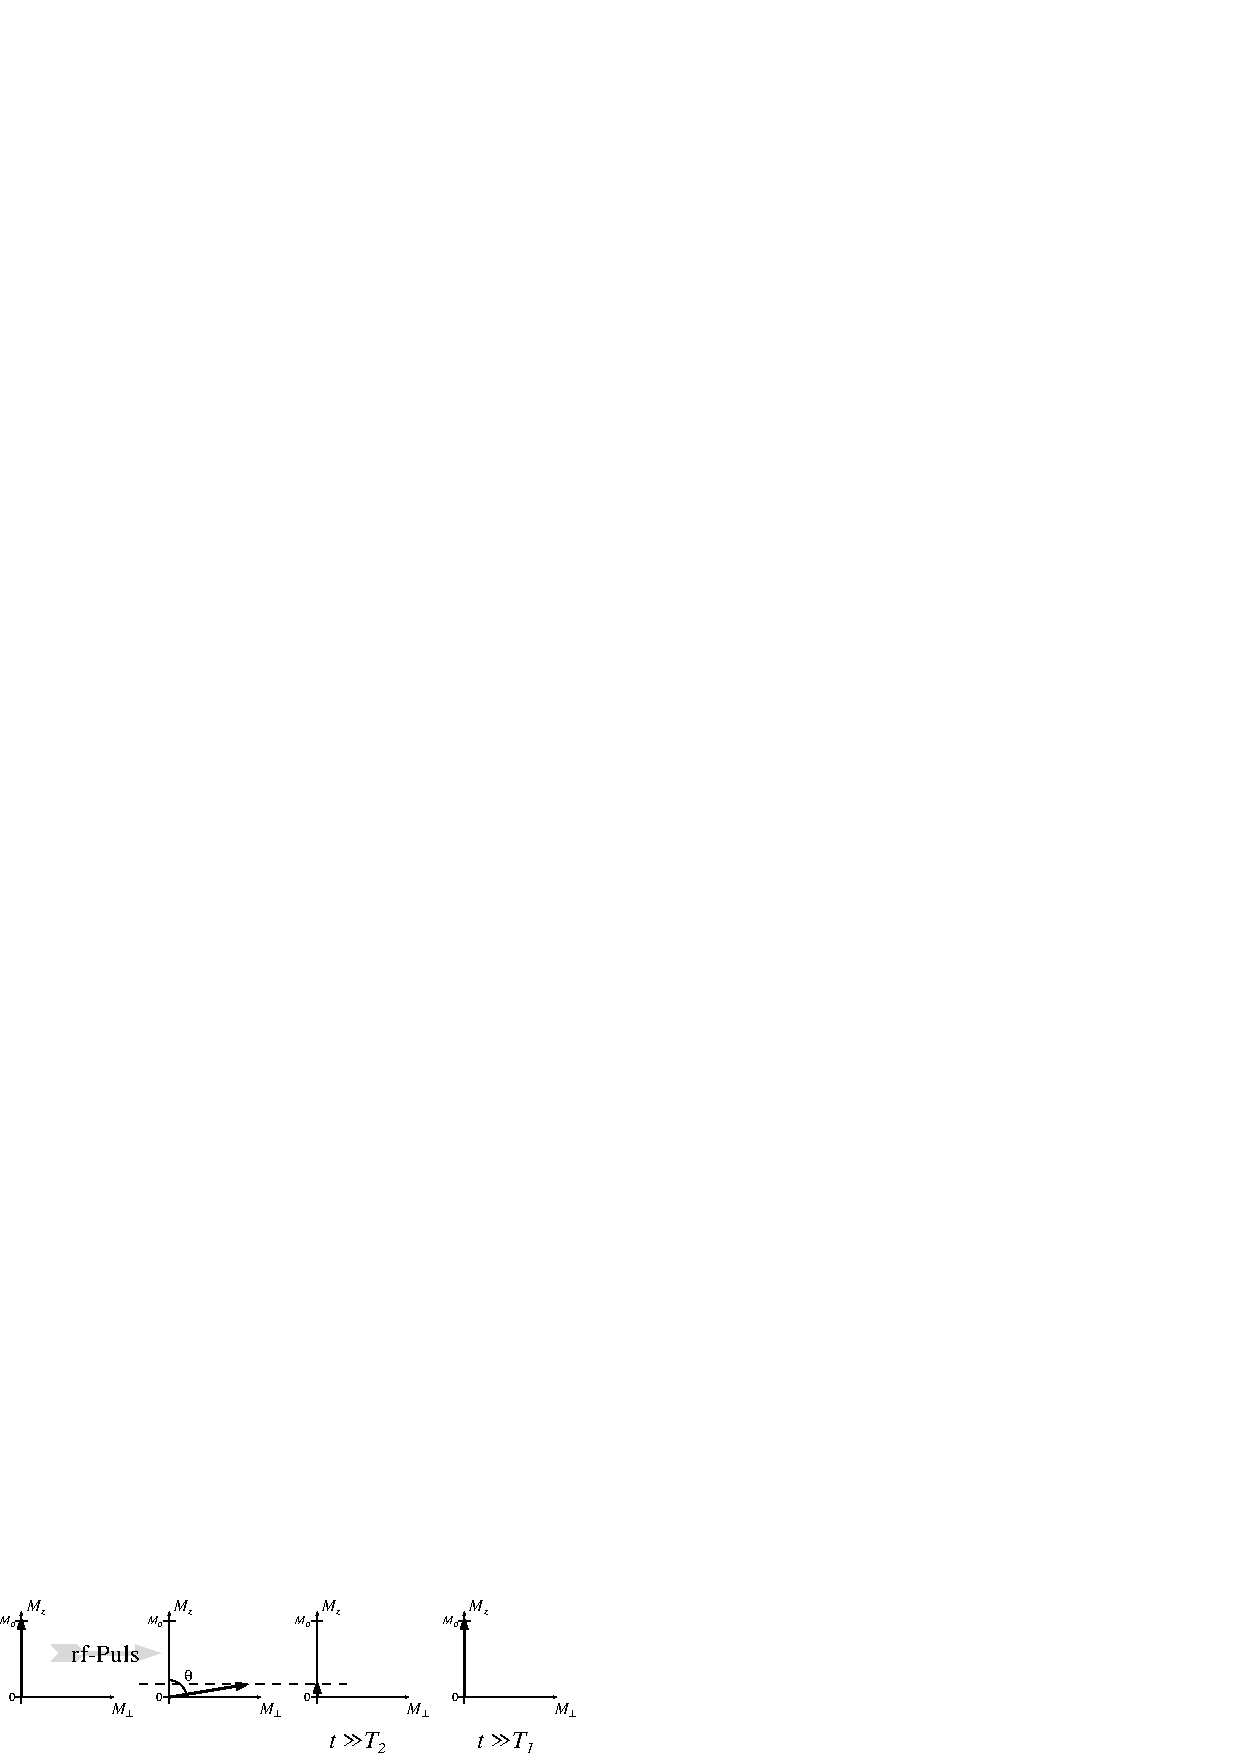
\includegraphics[bb=0 0 277 77,scale=1.44]{drawings/relaxation}$$
	\caption[Schema der Kernspinrelaxation in Metallen]{{\upshape\bfseries Schema der Kernspinrelaxation in Metallen ($T_2 \ll T_1$)}. Dargestellt ist
		das Verhalten des Vektors der makroskopisch meßbaren Magnetisierung $\vec M$ der Probe im
		Laborsystem, wie es durch die Blochgleichung \eqref{eqn:bloch} vorgegeben wird.
		$M_\perp=\sqrt{M_x^2+M_y^2}$ stellt den Betrag der Komponente der Magnetisierung dar, die
		senkrecht zur $z$"=Richtung ist. Diese Komponente $M_\perp$ relaxiert nach der Auslenkung
		von $\vec M$ durch den HF"=Puls aufgrund der Dephasierung der einzelnen Spins mit der
		Konstante $\frac1{T_2}$ auf Null zurück (\emph{Spin"=Spin Relaxation}), der langsamere
		Energieaustausch zwischen dem Spinsystem und dem Wärmebad der Leitungselektronen findet
		für $t\gg T_2$ statt, währenddessen sich die Spintemperatur mit der Zeitkonstante
		$\frac1{T_1}$ der Temperatur der Leitungselektronen annähert
		(\emph{Spin"=Gitter Relaxation}).}
	\label{fig:relaxation}
\end{figure}

Nach dieser Differentialgleichung für $M_z$ ergibt sich mit den Randbedingungen
	\begin{equation}
		\lim_{t\rightarrow\infty}M_z(t)=M_0 \ttextt{und} M_z(t=0)=M_{z0} \ttextt{mit}\abs{M_{z0}}<M_0
	\end{equation}
ein exponentieller Abfall von $M_z$ auf den Wert der Magnetisierung im thermischen Gleichgewicht
mit dem Wärmebad $M_0=M_\mathrm{sat}P\left(\frac{B}{T}\right)$ hin:
	\begin{equation}
		\label{eqn:mzdecay}
		M_z(t) = M_0 - \bigl(M_0-M_{z0}\bigr)\exp\left\{-\frac{t}{T_1}\right\}
	\end{equation}
Für einen beliebigen Tippingwinkel $\theta$ ergibt sich für die Werte der Magnetisierung parallel
und senkrecht zum äußeren Magnetfeld $B_0$ nach dem ersten HF"=Puls (zur Zeit $t=0$):
	\begin{align}
		M_z(t=0) &= M_0\cos\theta\\
		M_0 \propto M_\perp(t=0) &= \sqrt{\left.M_x(t=0)\right.^2+\left.M_y(t=0)\right.^2} = M_0\sin\theta\label{eqn:t1_m0}
	\end{align}
Dieser erste HF"=Puls dient dazu, das Spinsystem definiert aus dem Gleichgewicht auszulenken. Mit Hilfe
des zweiten HF"=Pulses ist es dann möglich, die momentane zeitliche Entwicklung der Relaxation der
$z$"=Komponete der Magnetisierung abzufragen.

Für die zeitliche Entwicklung von $M_z$ nach dem ersten HF"=Puls gilt:
	\begin{equation}
		M_z(t) = M_0 \left[1-\left(1-\cos\theta\right)\exp\left\{-\frac{t}{T_1}\right\}\right]
	\end{equation}
Um dies nun zu messen, strahlt man nach einer variablen Verzögerungszeit $dt$ einen zweiten
HF"=Puls mit demselben Tippingwinkel $\theta$ zur Abfrage der momentanen Entwicklung von $M_z(t)$
ein. Danach ist der Betrag der $z$"=Komponente der Magnetisierung zum Zeitpunkt des Abfragepulses
$\abs{M_z(dt)}$ proportional zur Größe der Komponente $M_\perp$ der Magnetisierung senkrecht zum
äußeren Magnetfeld:
	\begin{equation}
		\label{eqn:t1messung}
		\abs{M_z(dt)}\propto M_\perp=\sin\theta \abs{M_z(dt)}=\sin\theta M_0
			\abs{1-\left(1-\cos\theta\right)\exp\left\{-\frac{dt}{T_1}\right\}}
	\end{equation}
Wenn man nun die Auswertung der Meßwerte simuliert und aus \eqref{eqn:t1messung} und
\eqref{eqn:t1_m0} den Quotienten $\frac{\abs{M_z(dt)}}{M_0}$ bildet und dann, um einen
exponentiellen Abfall zu erhalten, $1-\frac{\abs{M_z(dt)}}{M_0}$ über $dt$ aufträgt, erhält man
einen Verlauf, der in Abbildung~\ref{fig:t1messung1} abhängig vom Tippingwinkel $\theta$ der
HF"=Pulse dargestellt ist.
 \begin{figure}[htp]
		$$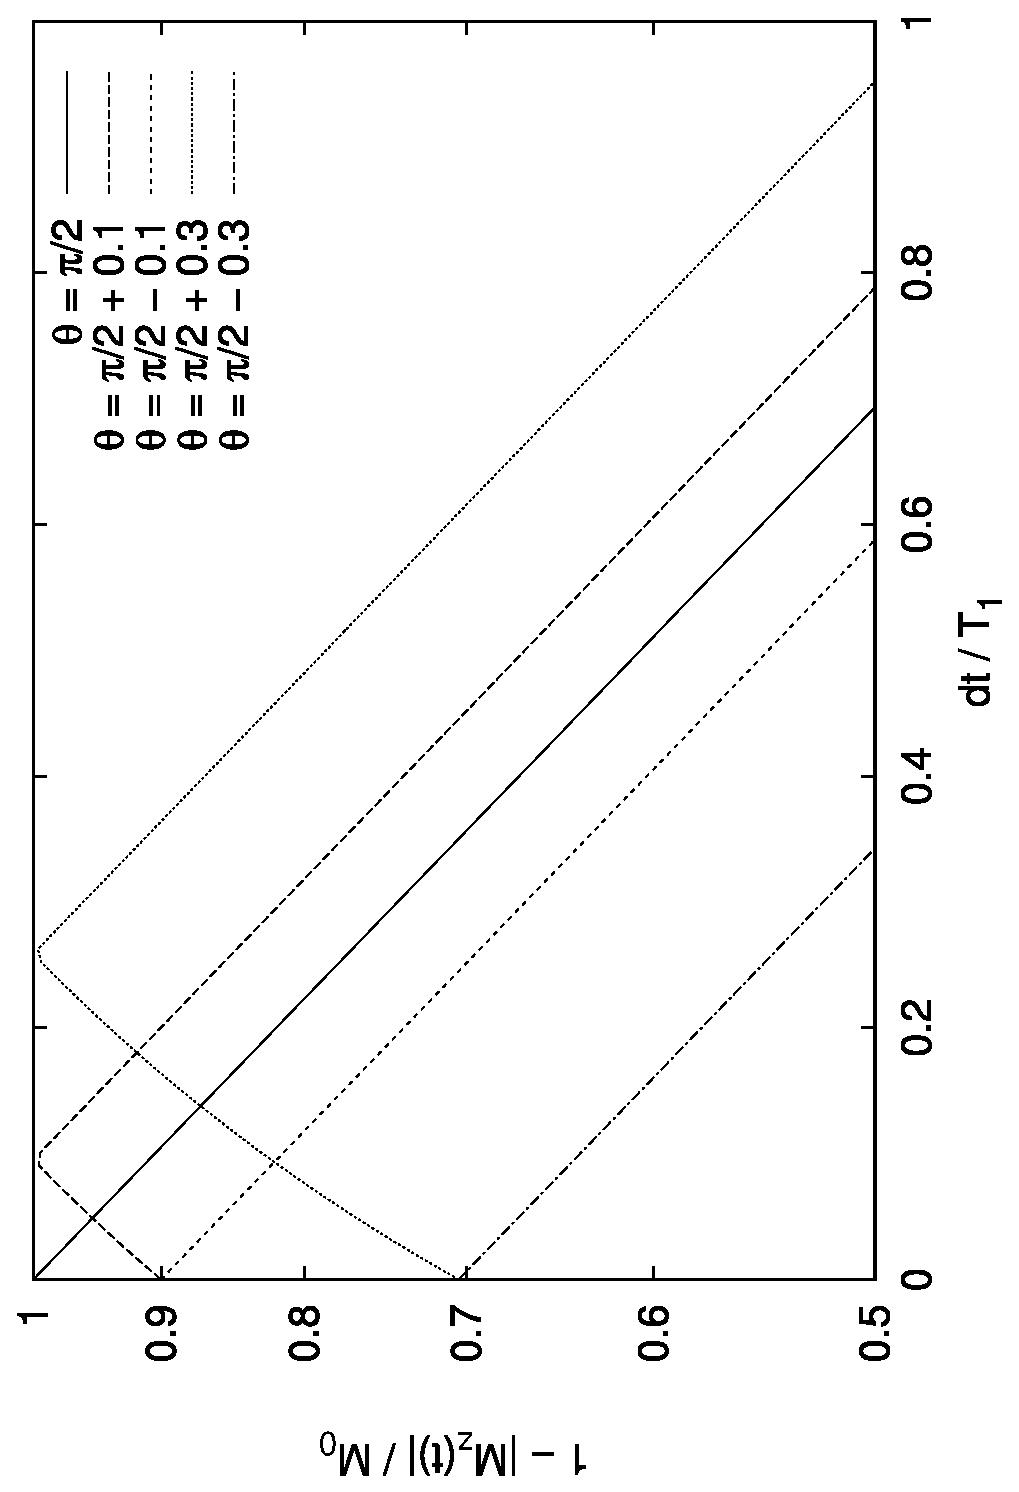
\includegraphics[angle=-90,width=\midwidth]{plots/t1_messung1}$$
	\caption[Theoretischer Verlauf der Meßergebnisse der $T_1$"=Messung]{{\upshape\bfseries
			Theoretischer Verlauf der Meßergebnisse der $T_1$"=Messung} in der verwendeten
			Auftragung $1-\frac{\abs{M_z(dt)}}{M_0}$ über $dt$ bei Abweichung
			vom Tippingwinkel $\theta=90$°. Den Knick bei kleinem $dt$ erhält man, wenn man das System
			"`übertippt"', d.\ h.\ bei $\theta>90$°. Die Auswirkungen dieses Verlaufs auf die
			erhaltenen Meßpunkte zeigen sich für das aufgrund des Skineffekts vorhandene
			inhomogene Tipping bei den durchgeführten Messungen.}
		\label{fig:t1messung1}
 \end{figure}
Demnach kann man also nach dem zweiten HF"=Puls ein Spulensignal messen, dessen
Resonanzlinienamplitude proportional zum Wert der mittleren Magnetisierung in $z$"=Richtung zum
Zeitpunkt des zweiten Pulses ist. Man hat also hier die Möglichkeit, die zeitliche Entwicklung der
Relaxation der Magnetisierung $M_z$ zu bestimmen. Ein Nachteil dieser Methode ist jedoch, daß man
mit jeder derartigen Zwei"=Puls"=Sequenz nur jeweils eine Verzögerungszeit $dt$ messen kann und
danach wieder auf die vollständige Relaxation von $M_z$, die mehrere $T_1$
dauert, warten muß. 
Dies ist bei Messungen mit Temperaturen unter etwa 1 mK problematisch, da die
$T_1$"=Relaxationszeiten auf Werte über 15 min ansteigen. Während der Wartezeit zwischen den
Pulssequenzen driftet die Temperatur der Kernstufe (= Wärmereservoir des Experiments) zu höheren
Temperaturen, was bei der Auswertung der Meßdaten berücksichtigt werden muß.

\subsubsection{Festlegung der Meßparameter}

Wie aus Gleichung~\eqref{eqn:t1messung} ersichtlich ist, erhält man die größte Änderung im Signal
proportional $M_z(dt)$ für einen Tippingwinkel $\theta=90^\circ$. Da es sich bei der
\aug"=Probe jedoch um eine massive Metallprobe handelt, verhindert der auftretende Skineffekt ein
homogenes Tipping in die Tiefe der Probe hinein. Deshalb kann man nur von einem mittleren
Tippingwinkel $\theta$ sprechen. Hier wurde als Ersatz für einen
Tippingwinkel von 90° eine Anregung des Kernspinsystems gewählt, bei der man, wenn man sich von
schwachen Anregungen nähert, das erste Maximum in der Linienintensität erhält. Die Positionen
dieser "`90°"'"=Pulse sind in Abbildung~\ref{fig:tipping} eingezeichnet, in der die Amplituden der
Resonanzlinien nach Hochfrequenzpulsen mit verschiedenen Anregungsstärken dargestellt sind.

\begin{figure}[htp]
	$$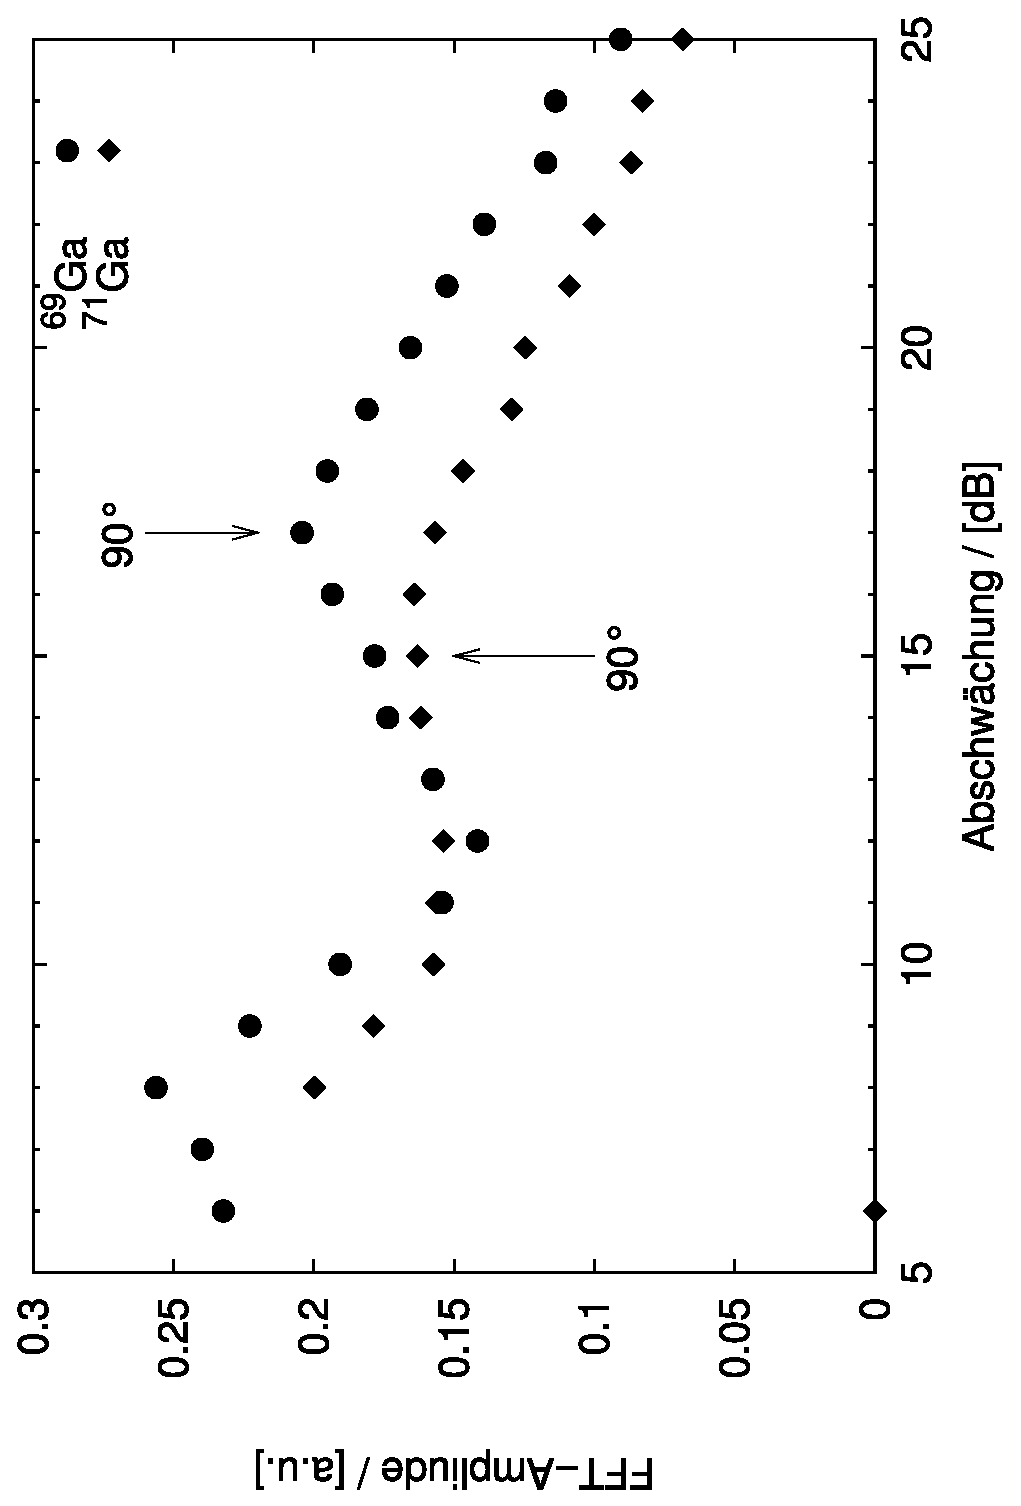
\includegraphics[angle=-90,width=\midwidth]{plots/tipping_aug1197_3}$$
	\caption[Bestimmung des Tippingwinkels $\theta$]{{\upshape\bfseries Bestimmung des Tippingwinkels $\theta$}. Die Amplitude der jeweiligen
		NMR"=Linie ist über der variierten Abschwächung der Amplitude des Pulses bei einer Anregungsfrequenz von
		4.184 MHz ($^{69}$Ga) bzw.\ 5.318 MHz ($^{71}$Ga) und einer Pulsdauer von 30
		Perioden aufgetragen. Zusätzlich sind die für die $T_1$"=Messung verwendeten Positionen der
		"`90°"'"=Pulse eingezeichnet. Diese Messung wurde bei einer stabilisierten Temperatur von ca.\ 60
		mK durchgeführt.}
	\label{fig:tipping}
\end{figure}

%%%%%%%%%%%%%%%%%%%%%%%%%%%%%%%%%%%%%%%%%%%%%%%%%%%%%%%%%%%%%%%%%%%%%%%%%%%%%%%%%%%%%%%%%%%%%%%%%%

\subsubsection{Messung der Spin"=Gitter Relaxationzeit $T_1$}

Es wurde abwechselnd an den Galliumisotopen $^{69}$Ga und $^{71}$Ga die Spin"=Gitter Relaxation wie
oben beschrieben gemessen. Die FIDs nach beiden HF"=Pulsen in der Sequenz wurden mit einem
Speicheroszilloskop aufgenommen und vom Computer eingelesen und zur Auswertung abgespeichert.
Zwischen den Pulssequenzen wurde eine Wartezeit eingehalten, die in der Größenordnung
von $5T_1$ liegt, damit die Magnetisierung der Galliumisotope wieder vollständig auf ihren
Gleichgewichtswert zurückrelaxieren kann. Bei einer Wartezeit von $5 T_1$ zwischen den
Sequenzen ergibt sich ein Fehler von $e^{-5}=0.0067$, also von unter einem Prozent, für die
Messung von $M_0$. Die
Verzögerungszeiten $dt$ wurden so gewählt, daß sie den Bereich von $0$s bis $3T_1$ gleichmäßig
abdecken. Bei späteren Messungen wurden die Wartezeiten zwischen den Pulssequenzen und die zu
messenden Verzögerungszeiten $dt$ automatisch vom Meßprogramm für die jeweilige Temperatur, aus der
in der ihrer Größenordnung bereits bekannten Spin"=Gitter Relaxationzeit $T_1$ berechnet und
verwendet.

\subsubsection{Auswertung der Meßdaten}

Von den aufgenommenen FIDs wurden mittels Fouriertransformation (FFT) die Resonanzspektren in den
Frequenzbereichen der Gallium"= und Kupfer"=NMR"=Linien berechnet. Schließlich wurden die NMR"=Linien
dann noch an die vier Parameter
 \begin{itemize}
	\item Linienlage (in Hz)
	\item Linienbreite (in Hz)
	\item Absorption der Linie
	\item Dispersion der Linie
 \end{itemize}
einer Fouriertransformierten eines idealen FIDs angepaßt. Diese ideale Resonanzlinie erhält man aus
der Fouriertransformation des Produkts der exponentiell abfallenden Hüllfunktion mit einer
Sinusschwingung. Sie ist einer Lorentzlinie ähnlich (siehe Abb.~\ref{fig:Auswertung}).

 \begin{figure}[htp]
	\begin{center}
		\subfigure[aufgenommener freier Induktionszerfall der \aug"=Probe ({\bfseries Parameter}: $B_0=400$ mT
			, $\nu_{rf}=4.184$ MHz, $t_\mathrm{Puls}=7.2 µ$s, Abschwächung: 17 dB,
			Temperatur(Pt"=NMR): 6.1 mK)]{
				$$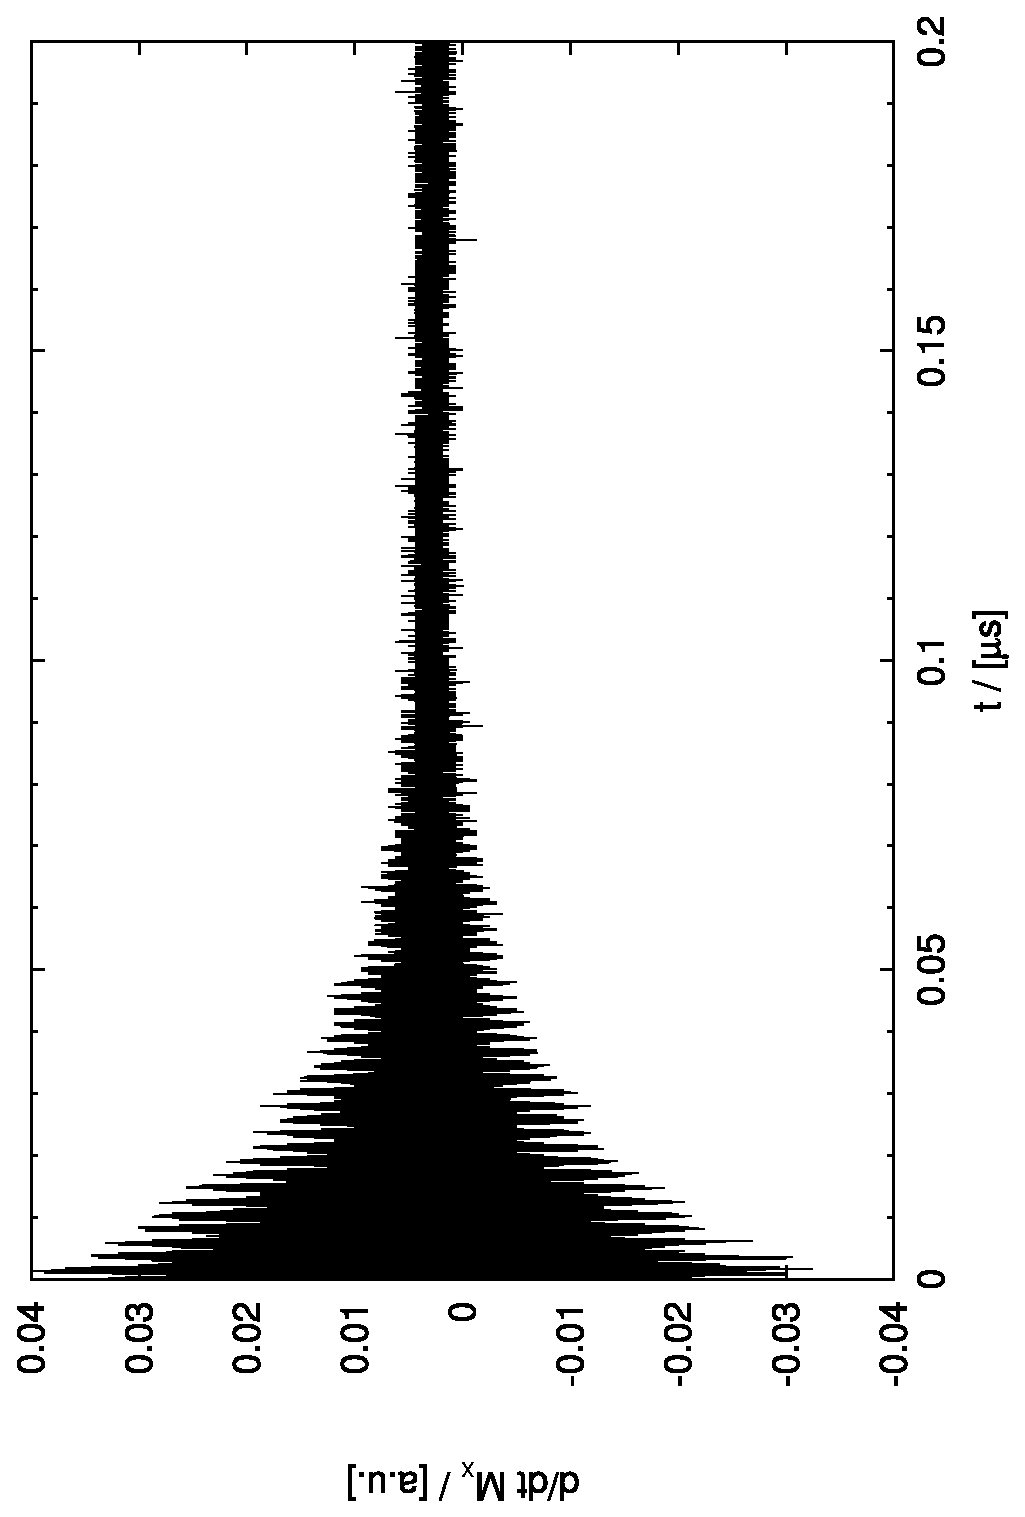
\includegraphics[angle=-90,width=\bigwidth]{plots/auswert1}$$}
		\subfigure[Frequenzspektrum des FID (Kreuze) mit NMR"=Linien"=Anpassung (durchgezogene Linie)]{
				$$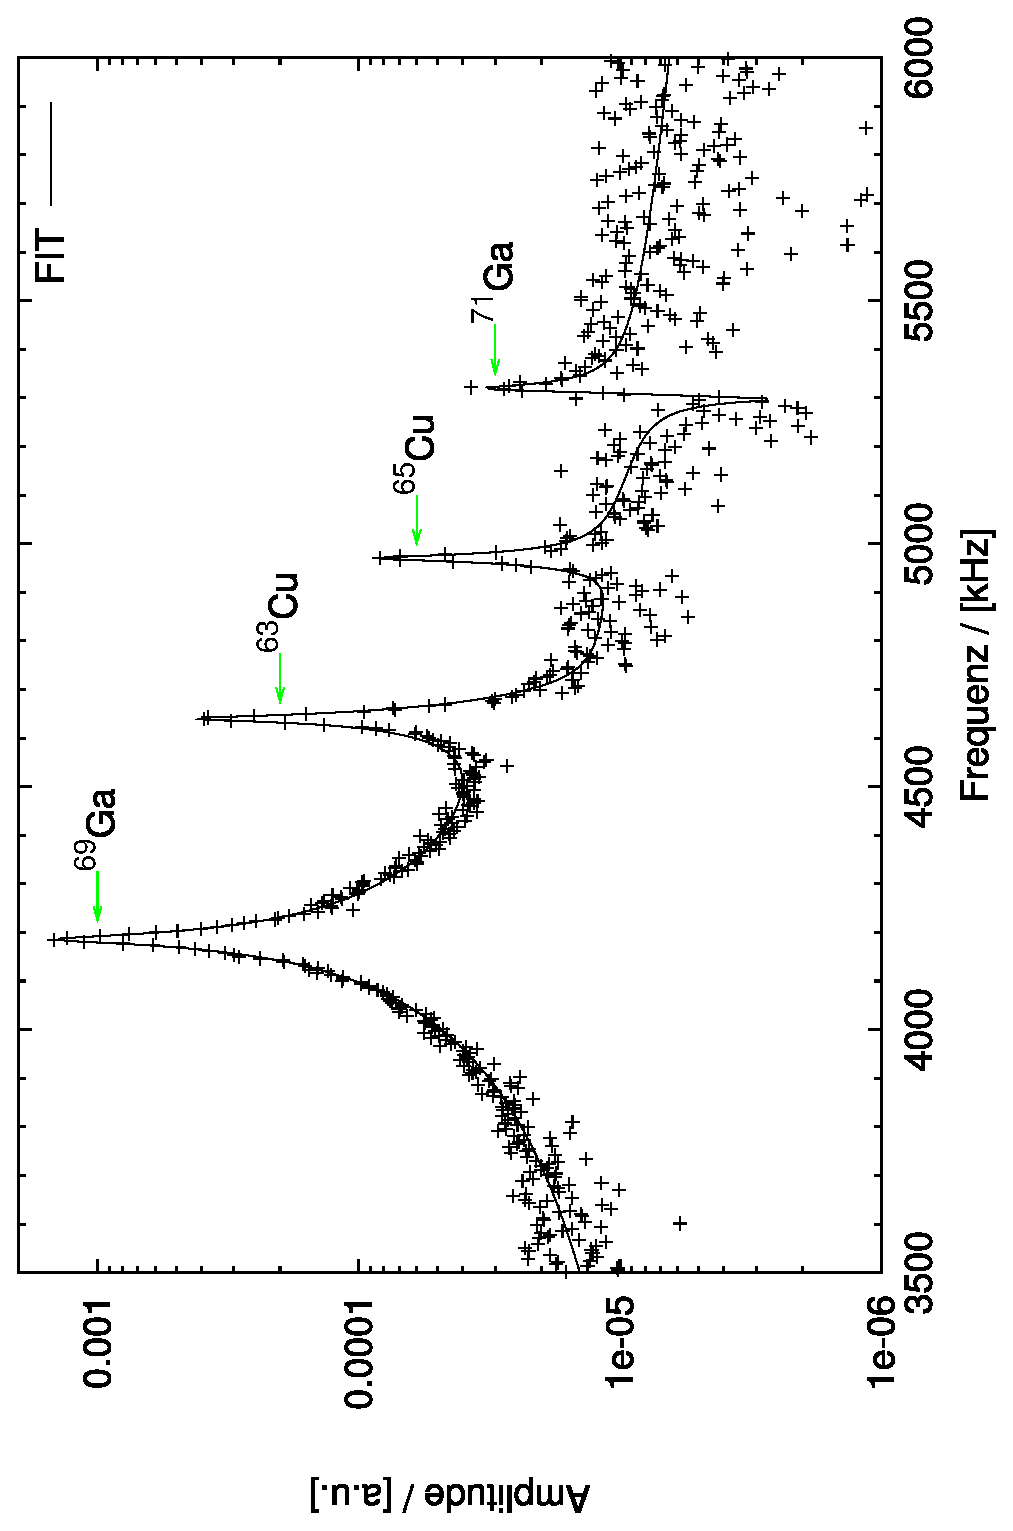
\includegraphics[angle=-90,width=\bigwidth]{plots/auswert2}$$}
	\end{center}
	\caption[Ein gemessener freier Induktionszerfall aus der $T_1$"=Messung]{{\upshape\bfseries Ein
		gemessener freier Induktionszerfall aus der $T_1$"=Messung.} Im
		berechneten Frequenzspektrum sieht man in der Reihenfolge von tiefen zu hohen Frequenzen
		hin die NMR"=Linien von $^{69}$Ga, $^{63}$Cu, $^{65}$Cu und $^{71}$Ga.}
	\label{fig:Auswertung}
	\enlargethispage{\baselineskip}
 \end{figure}

Die Amplitude der Resonanzlinie des betrachteten Isotops ergibt sich aus dem geometrischen Mittel
von Absorption und Dispersion. Sie ist bei konstanter Linienbreite proportional zur transversalen
Komponente der Magnetisierung $M_\perp$ des jeweiligen Isotopes nach Ende des HF"=Pulses. Daraus
erhält man folgende Informationen:
 \begin{itemize}
	\item Die Amplitude der Resonanzlinie im ersten FID ist proportional zur
		Gleichgewichtsmagnetisierung $M_0$.
	\item Die Amplitude der Resonanzlinie im zweiten FID ist dagegen proportional zum momentanen
		Wert der Magnetisierung $\abs{M_z(dt)}$ in $z$"=Richtung zu Beginn des zweiten HF"=Pulses.
 \end{itemize}
Da die Proportionalitätsfaktoren von $M_0$ und $\abs{M_z(dt)}$ identisch sind, kann man somit den
Quotienten der Magnetisierungen direkt aus dem Quotienten der Amplituden der Resonanzlinie
bestimmen:
	\begin{equation}
		\frac{\abs{M_t(dt)}}{M_0}=\frac{A_\mathrm{Puls 2}}{A_\mathrm{Puls 1}}
	\end{equation}
Wenn man nun $1-\frac{\abs{M_t(dt)}}{M_0}$ gegen die Verzögerungszeit $dt$ aufträgt, erhält man die
exponetielle Relaxation von $M_z$. Die Messungen, die bei konstanter Temperatur durchgeführt wurden,
können so einfach durch Bestimmung der Geradensteigung bei logarithmischer Auftragung von
$1-\abs{M_z(dt)}/M_0$ gegen die Verzögerungszeit $dt$ ausgewertet werden. In dieser Darstellung
ergibt sich die Spin"=Gitter Relaxationzeit nach \eqref{eqn:t1messung} aus dem Kehrwert der
Geradensteigung der Anpassungsgerade. Die in den Abbildungen \ref{fig:t1ergebnis1} und
\ref{fig:t1ergebnis2} gezeigten Fehlerbalken folgen aus dem statistischen Fehler des
least"=square"=Fits der NMR"=Linien im Frequenzspektrum und sind als Anhaltspunkt für den Meßfehler
in der logarithmischen Darstellung zu betrachten.

In Abbildung~\ref{fig:t1ergebnis1} ist das Ergebnis der ersten Messung von $T_1$ bei einem Feld
$B_0=140$~mT dargestellt. Bei dieser Messung wurde die Größe $M_0$ nur einmal, zu Beginn der Meßreihe,
bestimmt. Bei den darauf folgenden Messungen von $T_1$ bei einem Feld $B_0=400$~mT wurden die FIDs
beider Pulse, wie oben beschrieben aufgezeichnet und man erhält daraus ein $M_0$ für jede
Pulssequenz.

 \begin{figure}[p]
	\begin{center}
		\subfigure[$T_1$ von $^{69}$Ga in \aug{} mit $B_0=400$ mT]{
			$$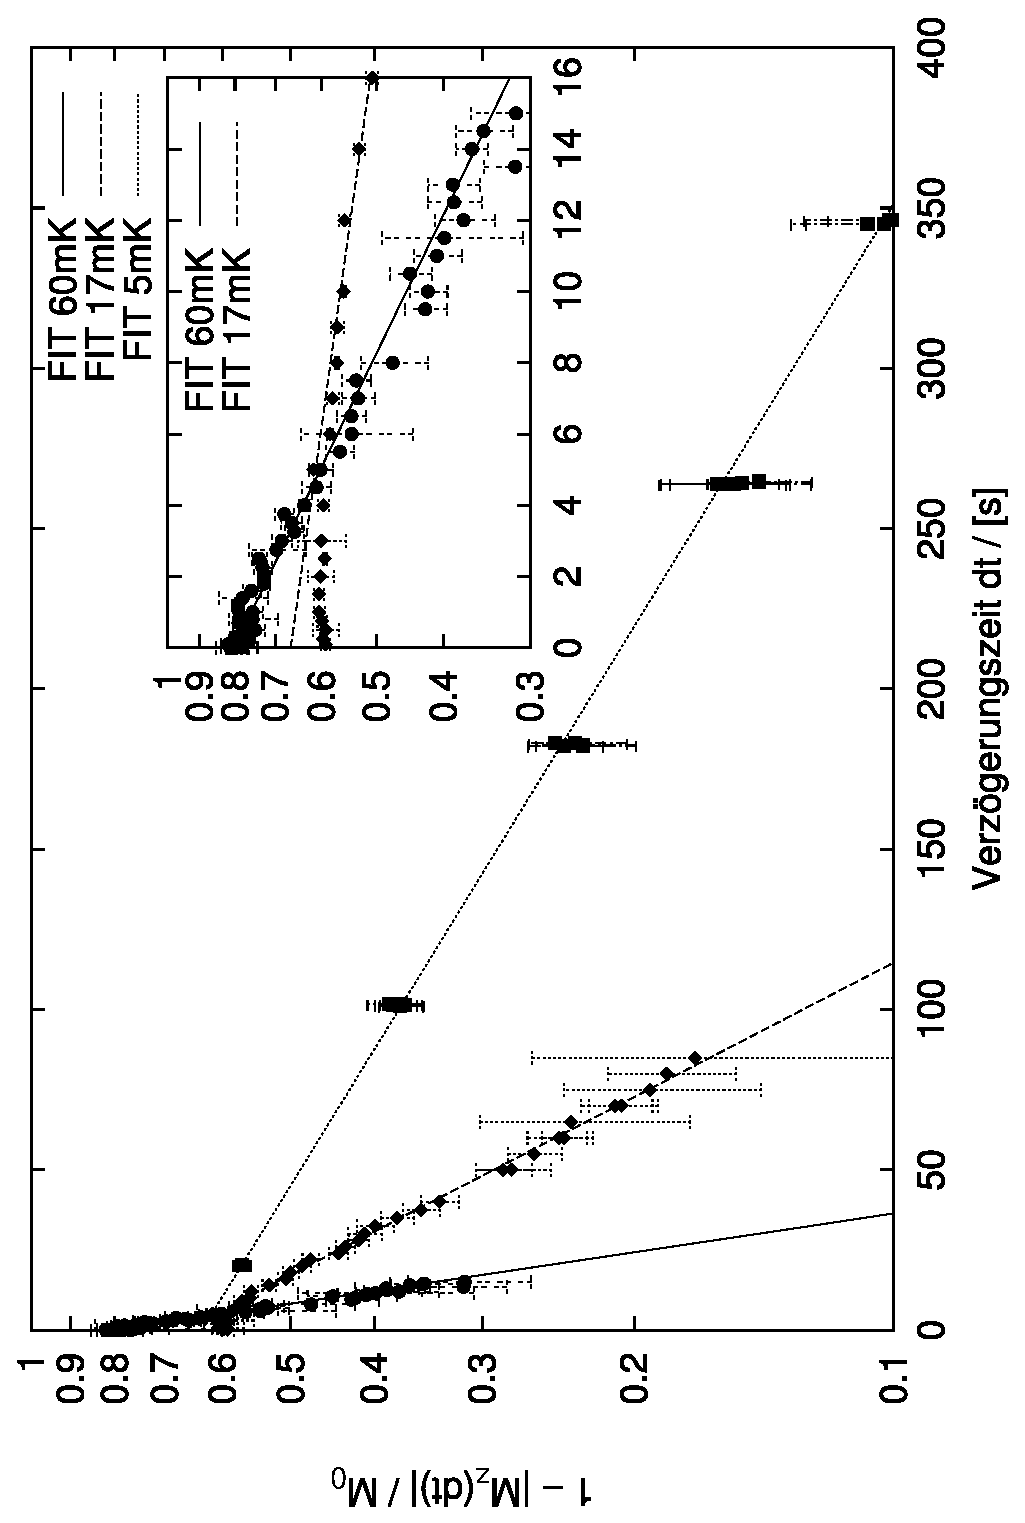
\includegraphics[angle=-90,width=\bigwidth]{plots/t1_auswert_1}$$}
		\subfigure[$T_1$ von $^{71}$Ga in \aug{} mit $B_0=400$ mT]{
			$$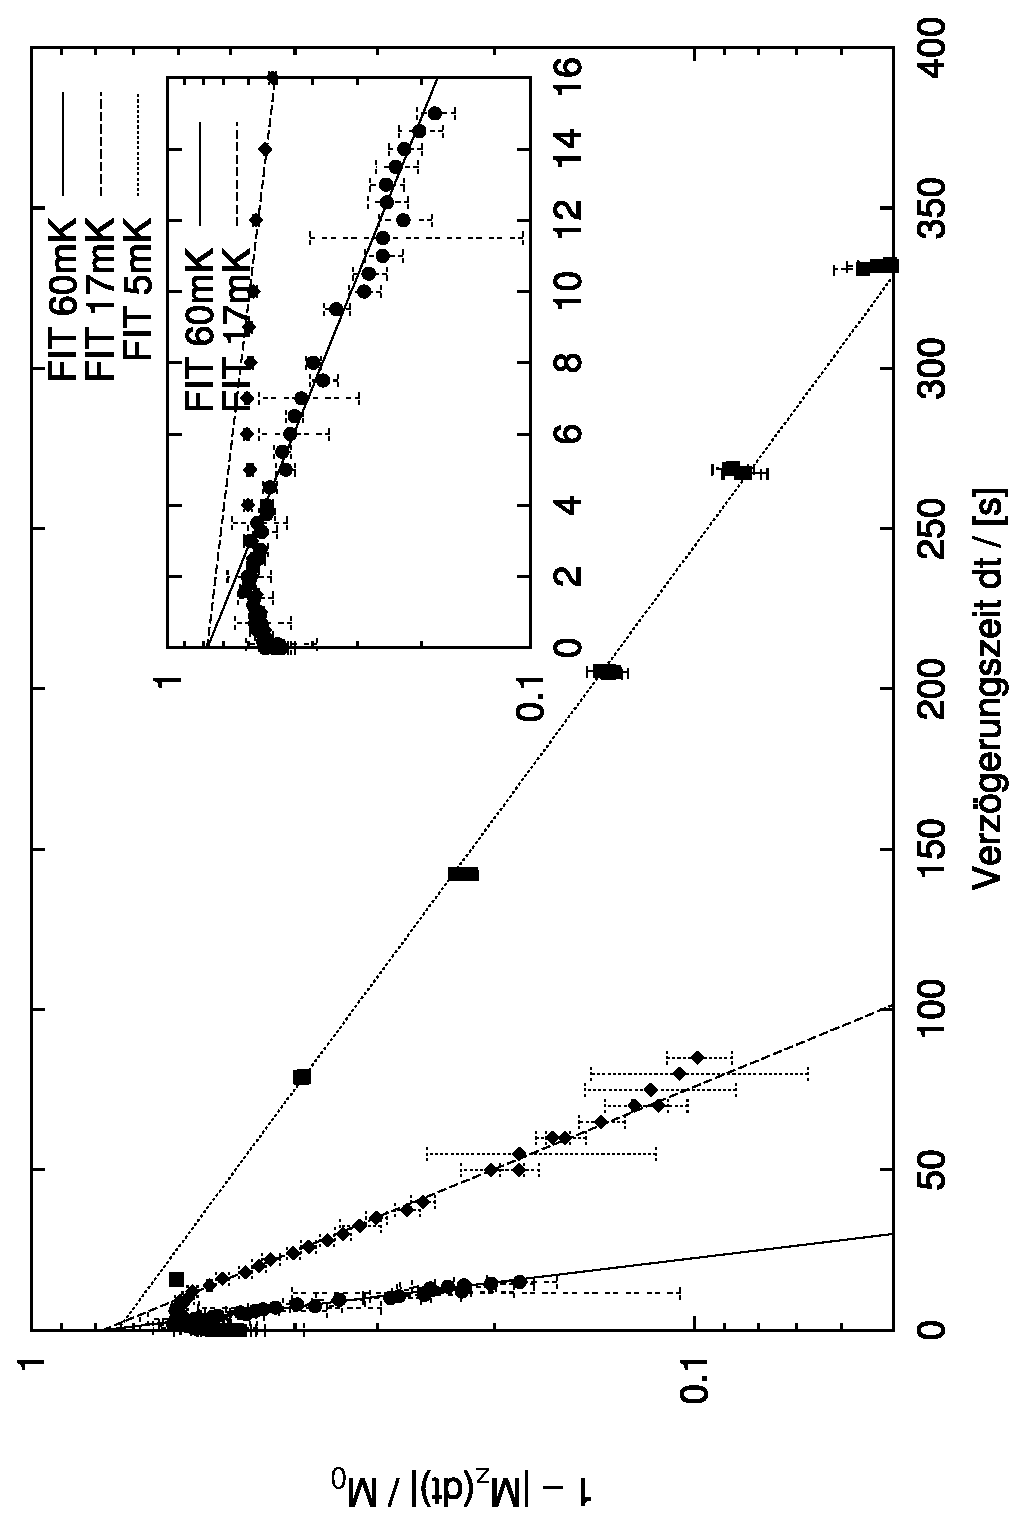
\includegraphics[angle=-90,width=\bigwidth]{plots/t1_auswert_2}$$}
	\end{center}
	\caption[Ergebnisse der $T_1$"=Messungen bei 400 mT]{{\upshape\bfseries Ergebnisse der
		$T_1$"=Messungen bei 400 mT}
		bei Temperaturen T=5.5 mK, 17 mK und 60 mK. Das Abweichen der Punkte von der
		Anpassungsgerade bei kurzen Verzögerungszeiten $dt$, das vor allem im Ausschnittsbild
		deutlich zu sehen ist, wird im Text diskutiert. [{\bfseries Parameter}: $B_0=400$~mT,
		$\nu(^{69}\mathrm{Ga})=4.184$~MHz, $\nu(^{71}\mathrm{Ga})=5.318$~MHz, Pulsdauer: 30
		Perioden, Abschwächung: $^{69}$Ga: 17 dB / $^{71}$Ga: 15 dB]}
	\label{fig:t1ergebnis2}
 \end{figure}

 \begin{figure}[htp]
	\begin{center}
		\subfigure[$T_1$ von $^{69}$Ga in \aug{}]{
			$$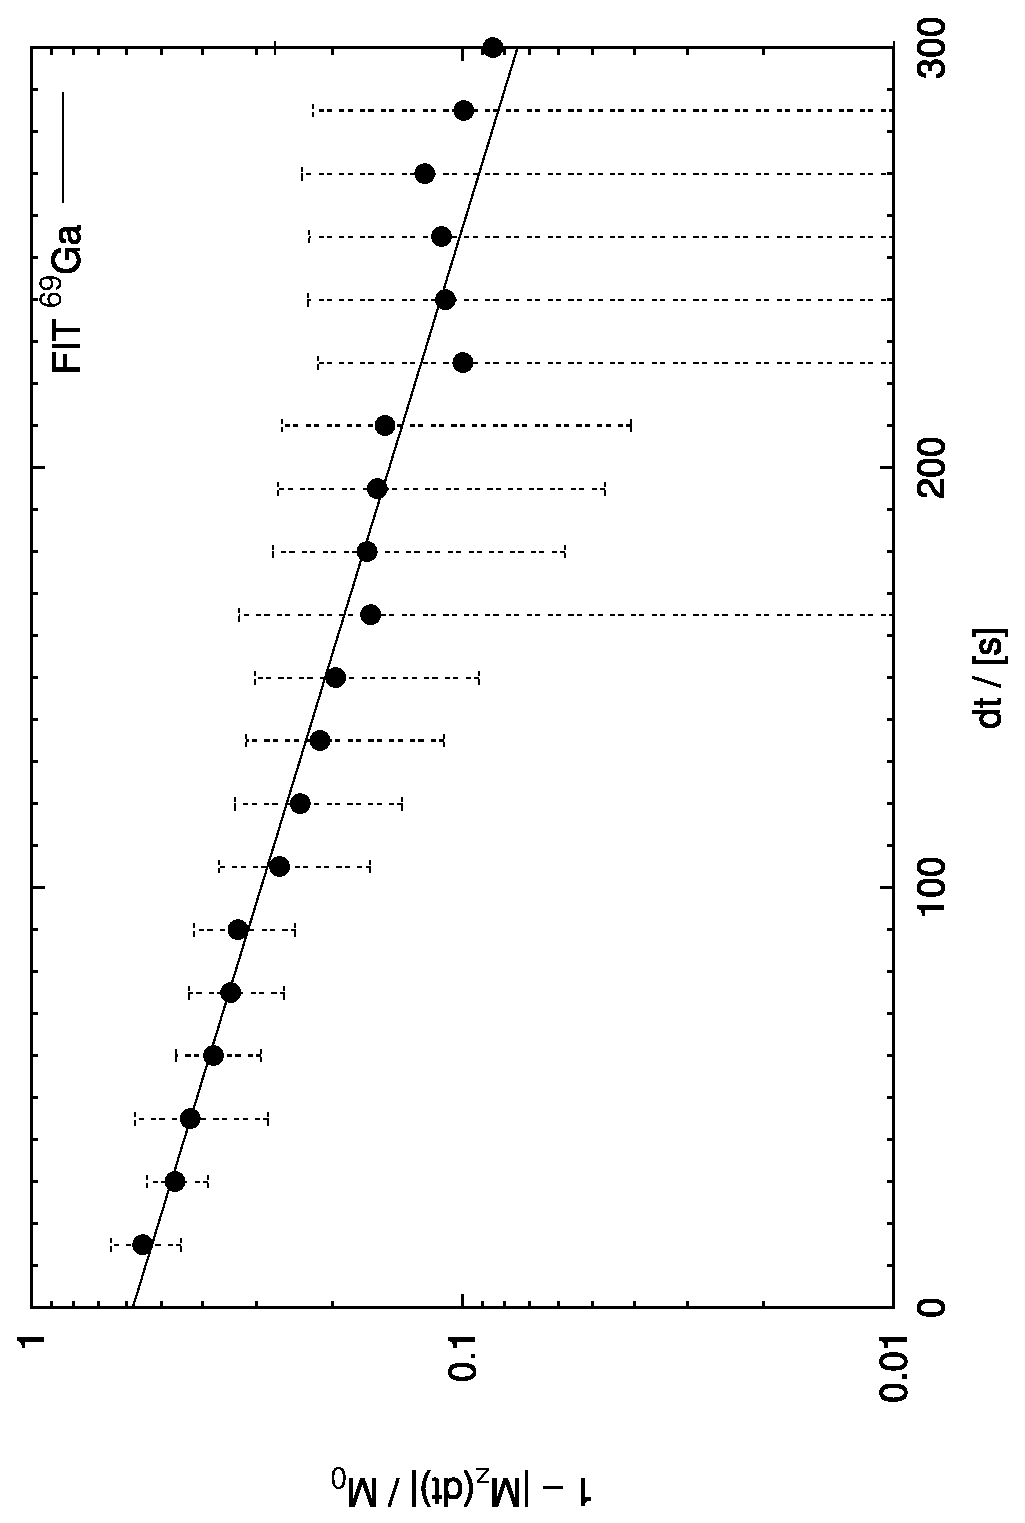
\includegraphics[angle=-90,width=\bigwidth]{plots/t1_aug0497d0_1}$$}
		\subfigure[$T_1$ von $^{69}$Ga in \aug{}]{
			$$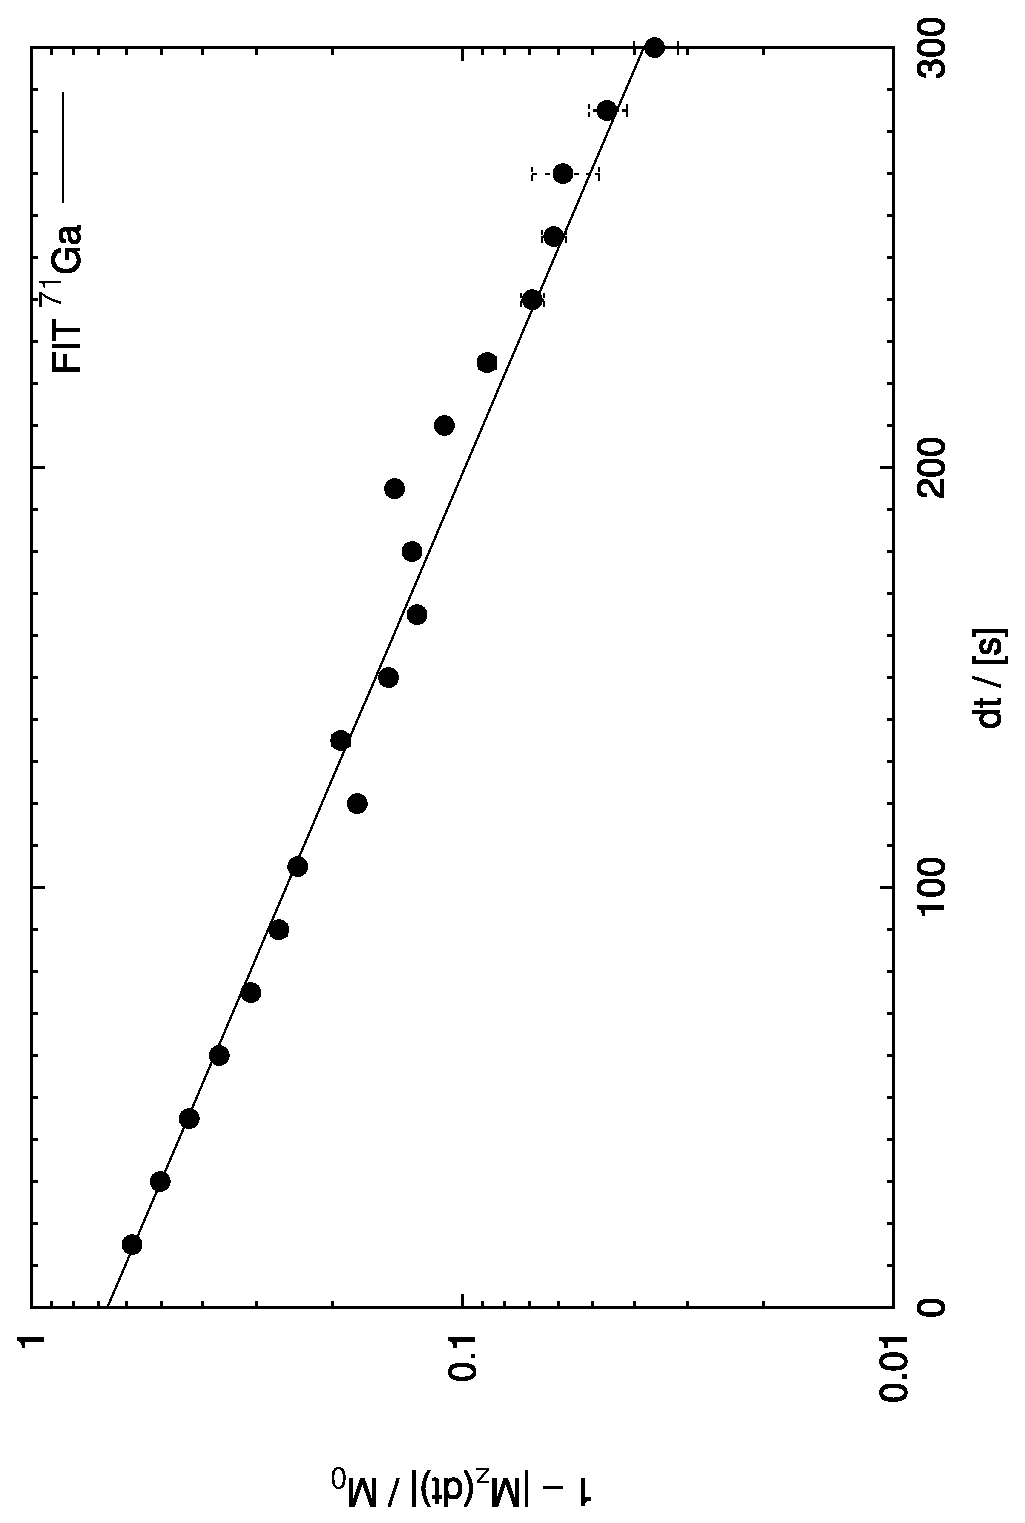
\includegraphics[angle=-90,width=\bigwidth]{plots/t1_aug0497d0_2}$$}	
	\end{center}
	\caption[Ergebnisse der $T_1$"=Messungen bei 140 mT]{{\upshape\bfseries Ergebnisse der
		$T_1$"=Messungen bei 140 mT} bei einer
		stabilisierten Temperatur von 5.5~mK. [{\bfseries Parameter}: $B_0=140$~mT,
		$\nu(^{69}\mathrm{Ga})=1.455$~MHz, $\nu(^{71}\mathrm{Ga})=1.850$~MHz, Pulsdauer: 10
		Perioden, Abschwächung: $^{69}$Ga: 20 dB / $^{71}$Ga: 18 dB]} 
	\label{fig:t1ergebnis1}
 \end{figure}

Die deutliche Abweichung der Meßpunkte von der Anpassungsgeraden bei kurzen Verzögerungszeiten,
die vor allem in den Ausschitten in Abbildung~\ref{fig:t1ergebnis2} zu sehen ist, soll hier kurz
diskutiert werden. In Abbildung~\ref{fig:t1messung1} sieht man den theoretischen Verlauf der
gemessenen Kurven für ein definiertes homogenes Tipping der Kernspins. Wenn man nun eine infolge
des Skineffekts gegebene reale Verteilung der Tippingwinkel annimmt, wird es zu einer Überlagerung
einer Kurvenschar nach Abbildung~\ref{fig:t1messung1} kommen, die durch die vorliegende Verteilung
von Tippingwinkel bestimmt ist. Die Abrundung im gemessenen Verlauf von
$1-\frac{\abs{M_z(dt)}}{M_0}$ bei kleinen Verzögerugszeiten $dt$ weist also auf die Existenz von
Tippingwinkeln größer als 90° hin. Da die Abweichungen von der Anpassungsgeraden bei der Messung
von $^{71}$Ga höher sind als bei $^{69}$Ga, kann man sogar sagen, daß die Spins von $^{71}$Ga
stärker angeregt wurden als die von $^{69}$Ga.

Anhand der Ergebnisse der bei konstanter Temperatur durchgeführten Messungen der Spin"=Gitter Relaxationzeit
kann man nun die Gültigkeit der Korringa"=Relation (nach Gleichung \eqref{eqn:korringa})
	\begin{equation}
		\label{eqn:korringarel}
		T_1 = \frac{\kappa}{T_\mathrm{el}} 
	\end{equation}
überprüfen. Aus der Anpassungsgeraden in Abbildung~\ref{fig:t1korringa} ergeben sich folgende
Werte für die Korringakonstanten der Galliumisotope in \aug{} bei einem Magnetfeld von $B_0=400$~mT:
	$$\begin{tabular}{|r|r|}\hline
		$^{69}$Ga:	& $1030\pm13$ mK s\\\hline
		$^{71}$Ga:	& $720\pm54$ mK s\\\hline
	\end{tabular}$$
 \begin{figure}[htp]
	$$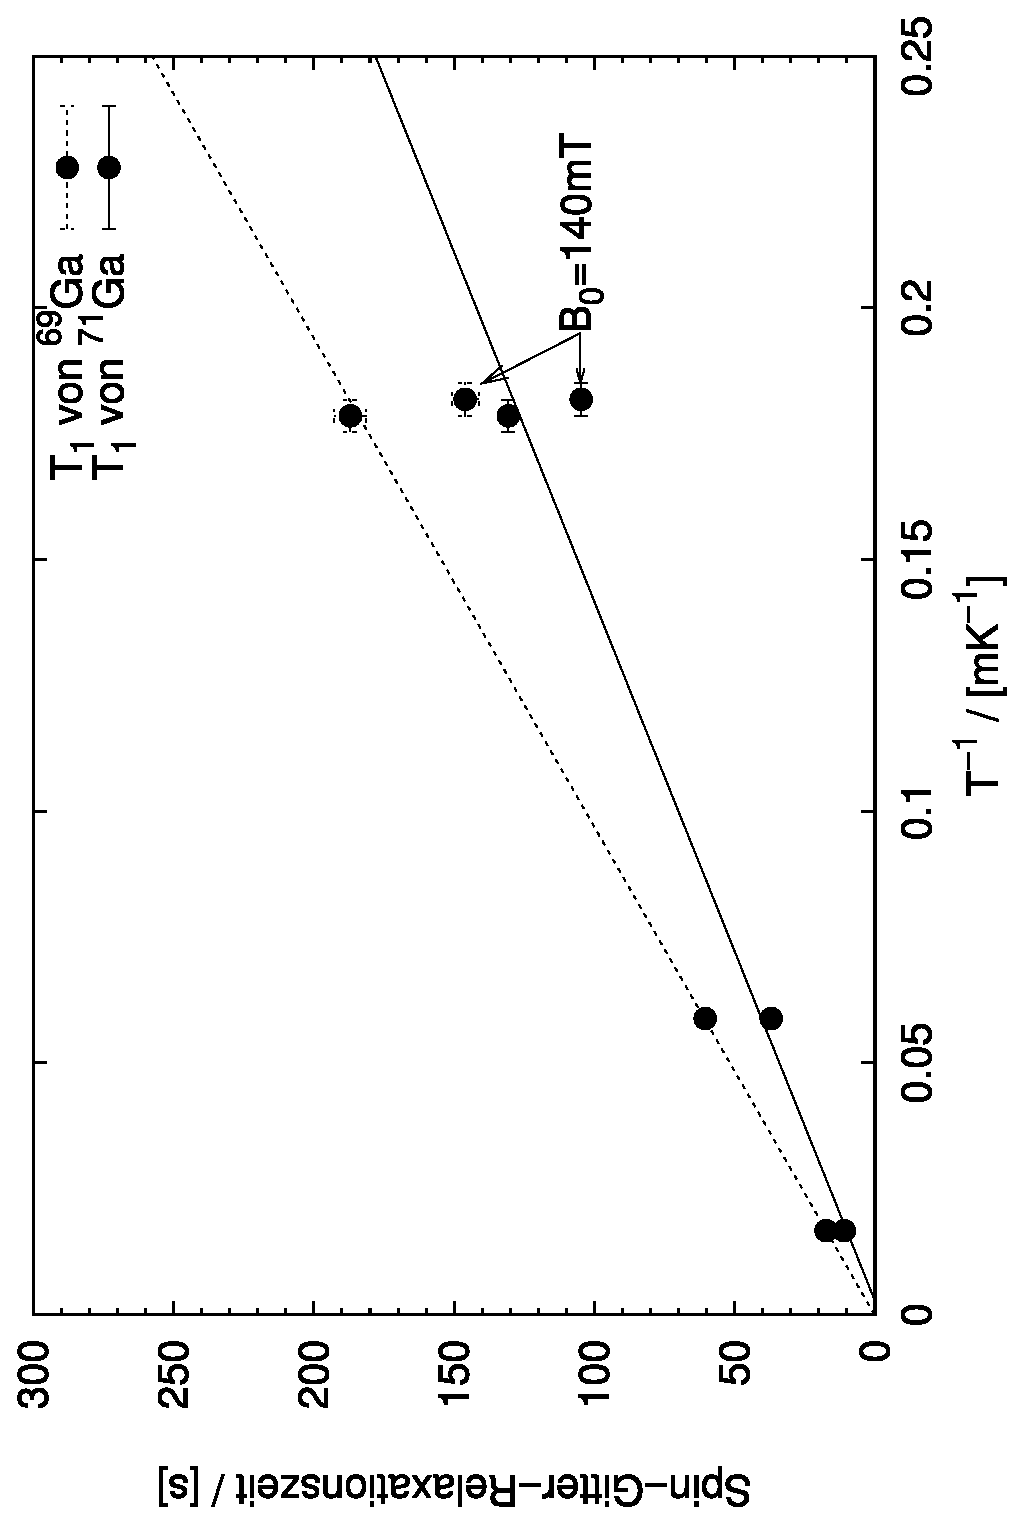
\includegraphics[angle=-90,width=\midwidth]{plots/t1_auswert2}$$
	\caption[Ergebnisse der $T_1$"=Messungen mit Anpassung an die
		Korringarelation]{{\upshape\bfseries Ergebnisse der $T_1$"=Messungen.} In der Auftragung der
		gemessenen Spin"=Gitter Relaxationzeiten über $\frac1{T}$ kann man die Gültigkeit der
		Korringarelation für die $T_1$"=Messung bei $B_0=400$~mT überprüfen. Die Korringa"=Konstante
		$\kappa$ ergibt sich aus der Geradensteigung der Anpassungsgerade. Die Meßpunkte der
		Messung bei $B_0=140mT$, für die sich eine geringere Korringakonstante ergibt, sind gekennzeichnet.}
	\label{fig:t1korringa}
 \end{figure}

Nachdem durch die Messungen bei konstanter Temperatur nachgewiesen wurde, daß die
Spin"=Gitter Relaxationzeit $T_1$ von Gallium in \aug{} eine Temperaturabhängigkeit nach der
Korringa"=Relation \eqref{eqn:korringarel} zeigt, kann man auch Messungen von $T_1$ durchführen,
in deren Verlauf die Temperatur der Probe nicht konstant ist.

\subsubsection{$T_1$"=Messungen bei variabler Probentemperatur}

Für die Messungen während der Aufwärmdrift nach Entmagnetisierung der Kupferkernstufe muß in der
Auswertung die sich während der Messung ändernde Temperatur der Probe zuerst aus den Meßwerten
bestimmt und dann bei der weiteren Auswertung berücksichtigt werden. Hierbei ist die
Vorgehensweise wie folgt:

Die Bestimmung der Temperatur der Probe (hier der Spintemperatur) geschieht nach dem Curie"=Gesetz aus der zur
Magnetisierung $M_0$ proportionalen Amplitude $A_\mathrm{Puls1}$ des FIDs nach dem ersten HF"=Puls.
	\begin{equation}
		\label{eqn:expcurie}
		T_\aug=\frac{c_\mathrm{Curie}}{M_0}\quad\Longrightarrow\quad c_\mathrm{Curie}=M_0\,T_\aug
	\end{equation}
Die Curiekonstante $c_\mathrm{Curie}$ kann man aus dieser Gleichung jedoch nicht bestimmen, da
$T_\aug$ ebenfalls unbekannt ist. Man kann aber die unbekannte Probentemperatur $T_\aug$ durch die
bekannte Temperatur am Pt"=NMR"=Thermometer $T_\mathrm{Pt}$ und einen unbekannten Temperaturgradienten
$\Delta(T_\aug,T_\mathrm{Pt})$ ausdrücken:
	\begin{equation}
		T_\aug=T_\mathrm{Pt} + \Delta(T_\aug,T_\mathrm{Pt})
	\end{equation}
Wieder in die Gleichung \eqref{eqn:expcurie} zur Bestimmung der Curie"=Konstante eingesetzt erhält man:
	\begin{equation}
		c_\mathrm{Curie}=M_0\,T_\mathrm{Pt} + M_0\,\Delta(T_\aug,T_\mathrm{Pt})
	\end{equation}
Nun kann man für hohe Temperaturen ($T\approx60mK$) den Beitrag des Temperaturgradienten
$\Delta(T_\aug,T_\mathrm{Pt})$ im Vergleich zur Temperatur $T_\mathrm{Pt}$ vernachlässigen.
Somit kann man die Curie"=Konstante zur Bestimmung der Temperatur der \aug"=Probe näherungsweise
berechnen:
	\begin{equation}
		c_\mathrm{Curie}\approx M_0\,T_\mathrm{Pt}
	\end{equation}
Anstelle von $M_0$ verwendet man die Amplitude $A_\mathrm{Puls1}$ der NMR"=Linie im FID des ersten
HF"=Pulses des jeweils gemessenen Galliumisotops. Die experimentelle Curie"=Konstante bestimmt man
durch Mittelung des Produkts von $T_\mathrm{Pt}$ und $A_\mathrm{Puls1}$ über alle Meßwerte mit
$T_\mathrm{Pt}>50mK$. Sobald eine Curie"=Konstante für eine Meßreihe an einem Isotop bestimmt ist,
läßt sich nach dem Curiegesetz \eqref{eqn:curie} die Probentemperatur für alle mit den gleichen
Parametern gemessenen FIDs aus dem jeweiligen $A_\mathrm{Puls1}$ bestimmen. Die Thermometrie der
Messung kann dann alleine durch die aus dem FID des Referenzpulses bestimmten Amplituden
$A_\mathrm{Puls1}$ erhalten werden. In Abbildung~\ref{fig:sampletemp} ist die so bestimmte
Temperatur $T_\aug$ der Probe über der Temperatur $T_\mathrm{Pt}$ aufgetragen, die mit dem
Platin"=NMR"=Thermometer gemessen wurde. Die unter 1~mK auftretenden Abweichungen können
verschiedene Ursachen haben. Zum einen steigt der Einfluß des Temperaturgradienten
$\Delta(T_\aug,T_\mathrm{Pt})$ bei tieferen Temperaturen an und zusätzlich verläßt man im Feld von
$B_0=400$~mT und bei Temperaturen unter 0.6~mK den Gültigkeitsbereich des Curie"=Gesetzes, das nur
eine Näherung der Brillouin"=Funktion für "`hohe"' Temperaturen darstellt (In
Abbildung~\ref{fig:frequenzshift} ist der Verlauf der Polarisation von \aug{} für tiefe
Temperaturen dargestellt).

Nun kann man analog zu den Messungen bei konstanter Temperatur die Meßwerte zu
$1-\frac{\abs{M_z(dt)}}{M_0}=1-\frac{A_\mathrm{Puls2}}{A_\mathrm{Puls1}}$
zusammengefaßt auftragen. Da die Gültigkeit der Korringarelation für Gallium in \aug{} im Rahmen der
Meßfehler im vorhergehenden Abschnitt gezeigt wurde, kann man nun zu einer von der Temperatur
unabhängigen Darstellung der Abs\-zis\-sen\-wer\-te übergehen. Hierzu multipliziert man die bekannte
Verzögerungszeit $dt$ mit der aus dem Curie"=Gesetz ermittelten Probentemperatur $T_\aug$ und
verwendet also eine Auftragung von $1-\frac{A_\mathrm{Puls2}}{A_\mathrm{Puls1}}$ über
$dt\,T_\aug$. Aus der Anpassung einer Exponentialfunktion $a\cdot e^{-b\cdot x}$ mit den
Parametern $a$ und $b$ an die so erhaltenen Punkte erhält man nun direkt die Korringakonstante
$\kappa$. Diese ergibt ich dann aus dem Kehrwert des Parameters $b$. Die Datenpunkte und die daran
angepaßte Exponentialfunktion sind in Abbildung~\ref{fig:t1plotTdt} sehen.

\begin{figure}[htp]
	\begin{center}
		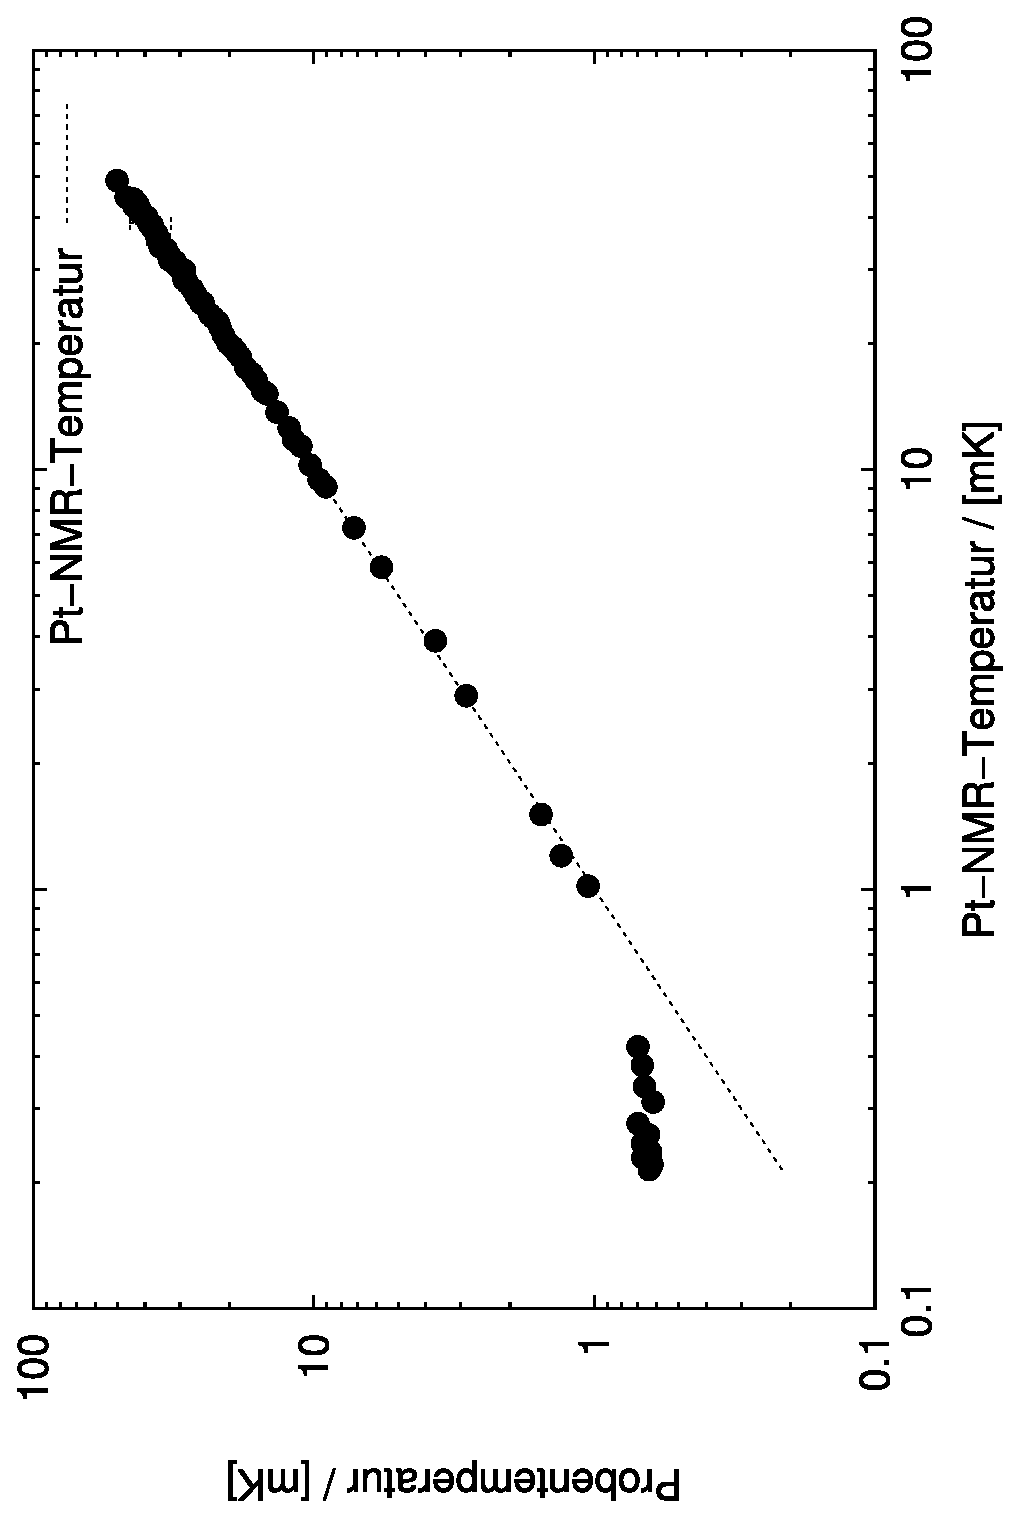
\includegraphics[angle=-90,width=\midwidth]{plots/t1_aug1197da_2}
	\end{center}
	\caption[Abweichung der mit Hilfe des Curie"=Gesetzes bestimmten
		Probentemperatur von der Pt"=NMR"=Temperatur]{{\upshape\bfseries Abweichung der mit Hilfe des Curie"=Gesetzes bestimmten
		Probentemperatur von der Pt"=NMR"=Temperatur.} Aus der $T_1$"=Messung während der
		Aufwärmdrift nach Entmagetisierung der Kupferkernstufe}
	\label{fig:sampletemp}
\end{figure}

\begin{figure}
	\begin{center}
			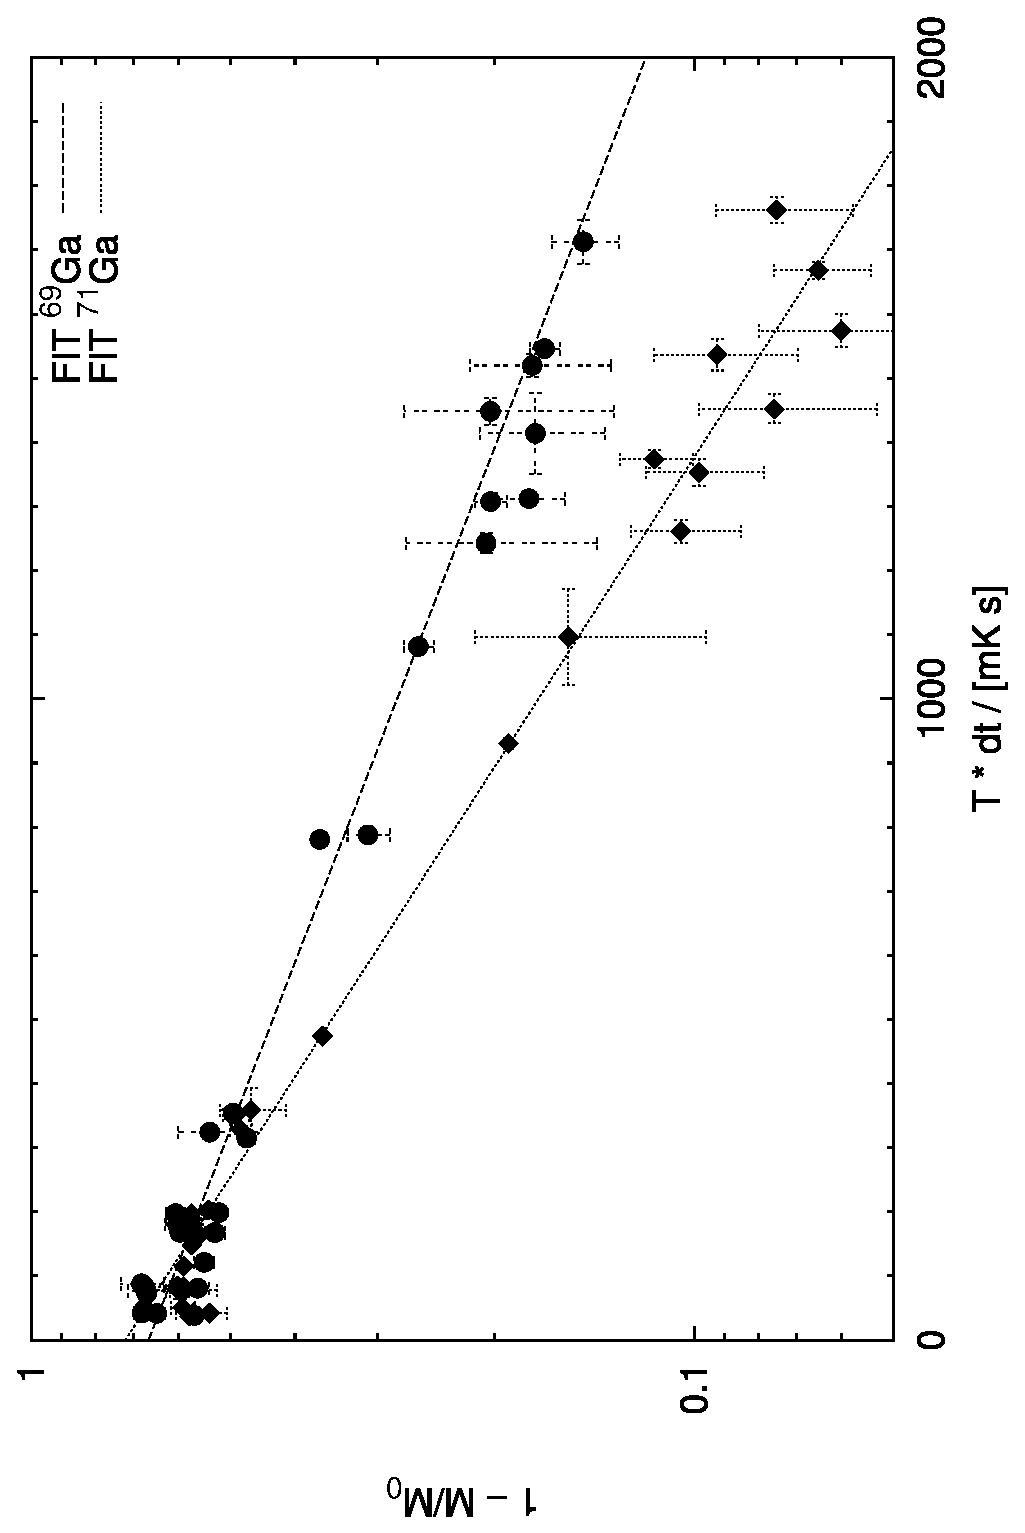
\includegraphics[angle=-90,width=\bigwidth]{plots/t1_aug1197da_3}
	\end{center}
	\caption[Temperaturunabhängige Auftragung von $1 -\frac{\abs{M_z(dt)}}{M_0}$ mit Anpassung an
		die Korringarelation.]{{\upshape\bfseries Temperaturunabhängige Auftragung von $1 -
		\frac{\abs{M_z(dt)}}{M_0}$ mit Anpassung an die Korringarelation.} Ergebnis der $T_1$"=Messung
		während der Aufwärmdrift nach Entmagetisierung der Kupferkernstufe. [{\bfseries Parameter:}  $B_0=400$~mT,
		$\nu(^{69}\mathrm{Ga})=4.184$~MHz, $\nu(^{71}\mathrm{Ga})=5.318$~MHz, Pulsdauer: 30
		Perioden, Abschwächung: $^{69}$Ga: 17 dB / $^{71}$Ga: 15 dB]}
	\label{fig:t1plotTdt}
\end{figure}

Aus dieser Messung erhält man einen Wert für die Korringakonstanten der Galliumisotope in \aug{} von 
	$$\begin{tabular}{|r|r|}\hline
		$^{69}$Ga:	& $1158\pm62$ mK s\\\hline
		$^{71}$Ga:	& $697\pm18$ mK s\\\hline
	\end{tabular}$$

%%%%%%%%%%%%%%%%%%%%%%%%%%%%%%%%%%%%%%%%%%%%%%%%%%%%%%%%%%%%%%%%%%%%%%%%%%%%%%%%%%%%%%%%%%%%%%%%%%

\subsection{Messung der Spin"=Spin Relaxationzeit T$_2$}
\label{sec:messungt2}

Die Spin"=Spin Relaxationzeit $T_2$ wurde mittels eines Spin"=Echos nach der Hahnschen Pulssequenz
(90°--$\tau$--180°) gemessen. Damit man die Amplitude von Spin"=Echos nach Zeiten $2\tau$ messen
kann, die in der Größenordnung der Zerfallszeit des FIDs liegen, wurde die effektive
Spin"=Spin Relaxationzeit $T_2^\ast$ mit Hilfe eines zusätzlichen starken Magnetfeldgradienten am
Probenort nach Gleichung \eqref{eqn:t2stern} verringert und somit der FID stark verkürzt. Dieser
Gradient wird mit Hilfe der Gradientenspule erzeugt, die sich am unteren Hauptmagneten befindet
(siehe Abb.~\ref{fig:Kryostat}). Der Strom durch die untere Gradientenspule wurde auf 50 A
eingestellt, woraus sich nach der Herstellerangabe ein Magnetfeldgradient von
$0.28\frac{\mathrm{mT}}{\mathrm{cm}\mathrm{A}}\cdot
50\mathrm{A}=14\frac{\mathrm{mT}}{\mathrm{cm}}$ ergibt.

\subsubsection{Die Linienform bei starken Magnetfeldgradienten}
Nach Anlegen des Magnetfeldgradienten änderte die Resonanzlinie deutlich ihre Form von der
bekannten NMR"=Resonanzlinie zu einer Doppellinie (zu sehen im Spektrum in
Abbildung~\ref{fig:t2messung}). Dies läßt sich folgendermaßen erklären: Durch den Skineffekt wird
bei der NMR an massiven Metallproben nur eine Oberflächenschicht mit der Dicke der Skintiefe
angeregt und auch detektiert. Da nun zusätzlich zum statischen Feld $B_0$ ein Magnetfeldgradient
in $z$"=Richtung an der Probe vorliegt, folgt daraus eine Verteilung von NMR"=Resonanzfrequenzen,
die von den Beiträgen der Probe zu verschiedenen $z$"=Komponenten bestimmt wird. Ein
einfaches Modell für die Auswirkungen des Skineffekts auf die Linienform ist ein dünnwandiges Rohr
mit dem Probenradius $R$ und Wandstärke $\delta$ in der Größenordnung der Skintiefe, für das der
Skineffekt vernachlässigbar und somit ein homogenes Tippingverhalten vorliegt. Es ergibt sich ein
radialer Beitrag zum NMR"=Signal, der durch das Produkt zweier Stufenfunktionen gegeben ist,
	\begin{equation}
		a(r) = \Theta\bigl(R-r\bigr)\Theta\bigl(\delta-(R-r)\bigr)
	\end{equation}
Wobei für den Abstand $r$ von der Proben"= oder Rohrachse in dem hier verwendeten Koordinatensystem
(siehe Abb~\ref{fig:gradlinform_a}) aufgrund der Zylindersymmetrie $r=\sqrt{y^2+z^2}$ gilt.
Der Beitrag zu einem bestimmten Magnetfeld ist wegen der Linearität von Gleichung~\eqref{eqn:resonanzbed}
proportional zur NMR"=Resonanzfrequenz. Bei dem vorhandenen Gradienten des Magnetfeldes in
$z$"=Richtung ist der Beitrag $b(z)$ zur Resonanzfrequenz somit proportional dem Integral von
$a(r)$ über $y$ bei fester $z$"=Koordinate:
	\begin{equation}
		\label{eqn:gradbeitrag}
		b(z) = \int\limits_{-R}^{+R}a(\sqrt{y^2+z^2})dy
	\end{equation}
Der Verlauf dieses Integrals in Abhängigkeit von der $z$"=Koordinate ist in
Abbildung~\ref{fig:gradlinform} dargestellt. Das Aussehen der Resonanzlinie im NMR"=Spektrum erhält man nun
aus der Überlagerung aller Beiträge $b\bigl(z(\nu_\mathrm{Larmor})\bigr)$ über die Probe hinweg.
Das heißt durch Faltung der Funktion in Abb~\ref{fig:gradlinform_b} mit einer NMR"=Resonanzlinie ohne
Magnetfeldgradient.

\begin{figure}[htp]
	\begin{center}
		\subfigure[Querschnitt durch die NMR"=Probe]{
			\label{fig:gradlinform_a}
			\parbox[c]{0.6\smallwidth}{\centering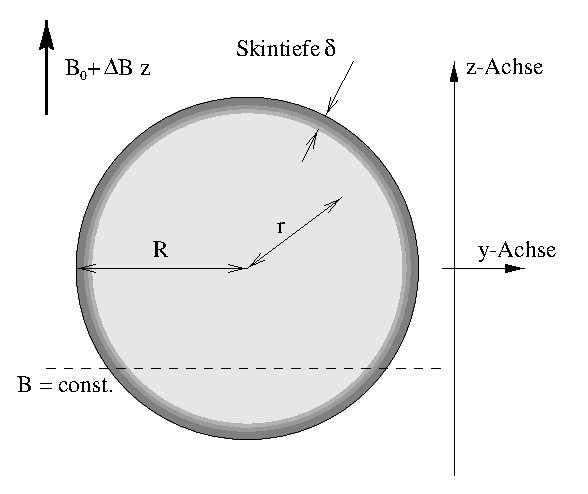
\includegraphics[width=0.6\smallwidth]{drawings/gradlinform}}}
		\subfigure[Verhalten von Gleichung \ref{eqn:gradbeitrag} für die Parameter $R=0.15$,
			$\delta=0.005$]{
			\label{fig:gradlinform_b}
			\parbox[c]{0.9\smallwidth}{\centering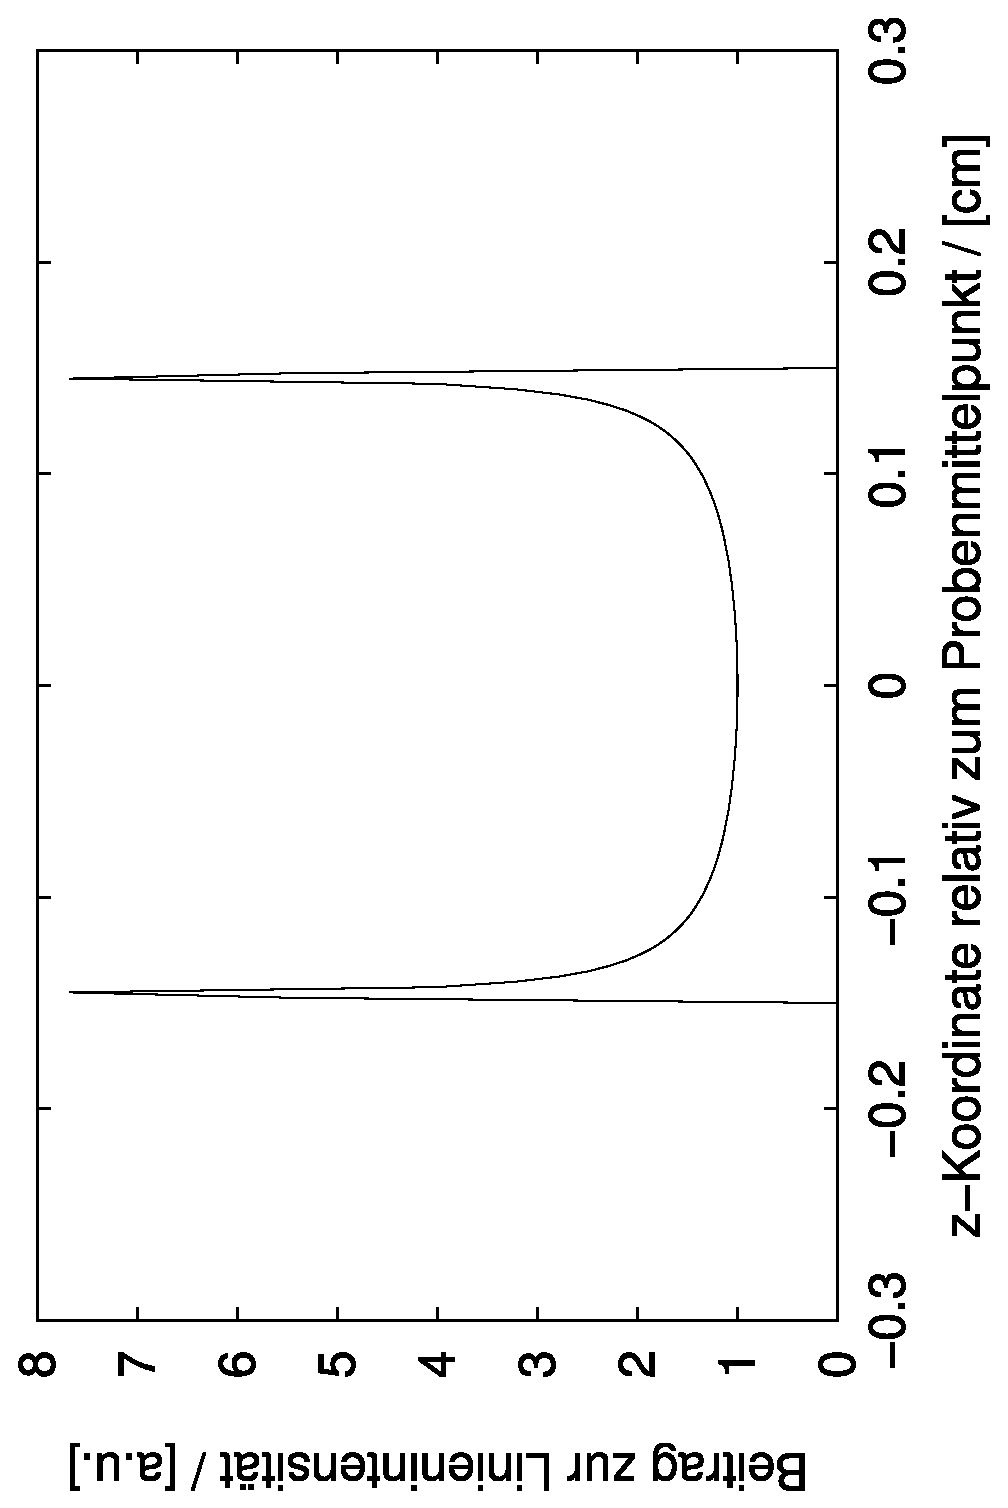
\includegraphics[angle=-90,width=0.9\smallwidth]{plots/gradlinform}}}
	\end{center}
	\caption[Erklärung der Änderung der Linienform durch einen Gradienten des
		Magnetfeldes]{{\upshape\bfseries Erklärung der Änderung der Linienform durch einen Gradienten des
		Magnetfeldes.} Im rechten Bild sieht man die Intensitätverteilung der Resonanzfrequenzen
		in $z$"=Richung über die Probe hinweg. Die wahre Form der NMR"=Linie ergibt sich durch
		Faltung einer NMR"=Resonanzlinie ohne Magnetfeldgradient mit der Funktion aus
		Gleichung~\eqref{eqn:gradbeitrag} im Frequenzraum. Die Umrechnung von der $z$"=Koordinate
		in eine Frequenz $\nu$ erfolgt bei bekanntem Gradienten nach Gleichung~\eqref{eqn:resonanzbed}. }
	\label{fig:gradlinform}
\end{figure}

Auf diese Weise kann man für das Modell den Magnetfeldgradienten aus dem Abstand der beiden
Spitzen der Resonanzlinie bestimmen. Aus Abbildung~\ref{fig:t2messung} ergibt sich für den Abstand
der Spitzen $\Delta\nu=61\pm20$~kHz. Für den Magnetfeldgradienten ergibt sich nun folgende Formel:
	\begin{equation}
		\nabla B=\frac{\Delta\nu}{\gamma\Delta z}=
			\frac{100\pm50\,\mathrm{kHz}}{13.001\frac{\mathrm{kHz}}{\mathrm{mT}}0.3\,\mathrm{cm}}=
			16\pm5\frac{\mathrm{mT}}{\mathrm{cm}}
	\end{equation}
Der so errechnete Wert stimmt innerhalb der Fehler mit der Herstellerangabe von
$14\frac{\mathrm{mT}}{\mathrm{cm}}$ bei einem Spulenstrom von 50~A für die Gradientenspule
überein.

\subsubsection{Durchführung der Messung}

Das Prinzip der Wirkung der 90°--$\tau$--180° Pulssequenz zur Messung der
Spin"=Spin Relaxationszeit $T_2$ ist aus Abbildung~\ref{fig:t2methode} ersichtlich. Die nach
dem ersten 90° HF"=Puls ausgelenkten Spins laufen aufgrund der vom Magnetfeldgradienten
verursachten unterschiedlichen Larmorfrequenzen auseinander. Nach der Zeit $\tau$ werden durch Einstrahlung
eines 180° HF"=Pulses die so dephasierten Spins in der $xy$"=Ebene umgeklappt. Da sich die Verteilung der
Larmorfrequenzen auf der Probe nicht ändert, wird der Prozeß des
Auseinanderlaufens der Kernspins wieder umgekehrt. Nach der Zeit $2\tau$ fokussieren die Spins
wieder bei einer Position, die zur Ausgangsposition um 180° phasenverschoben ist. Mit der
Probenspule detektiert man dann das Auftreten eines Spin"=Echos. Aus der Verringerung der Amplitude
einer NMR"=Resonanzlinie des Echos im Vergleich zur Amplitude der Resonanzlinie im FID nach dem 90°
HF"=Puls erhält man die intrinsische Spin"=Spin Relaxationzeit $T_2$.

 \begin{figure}[htp]
	$$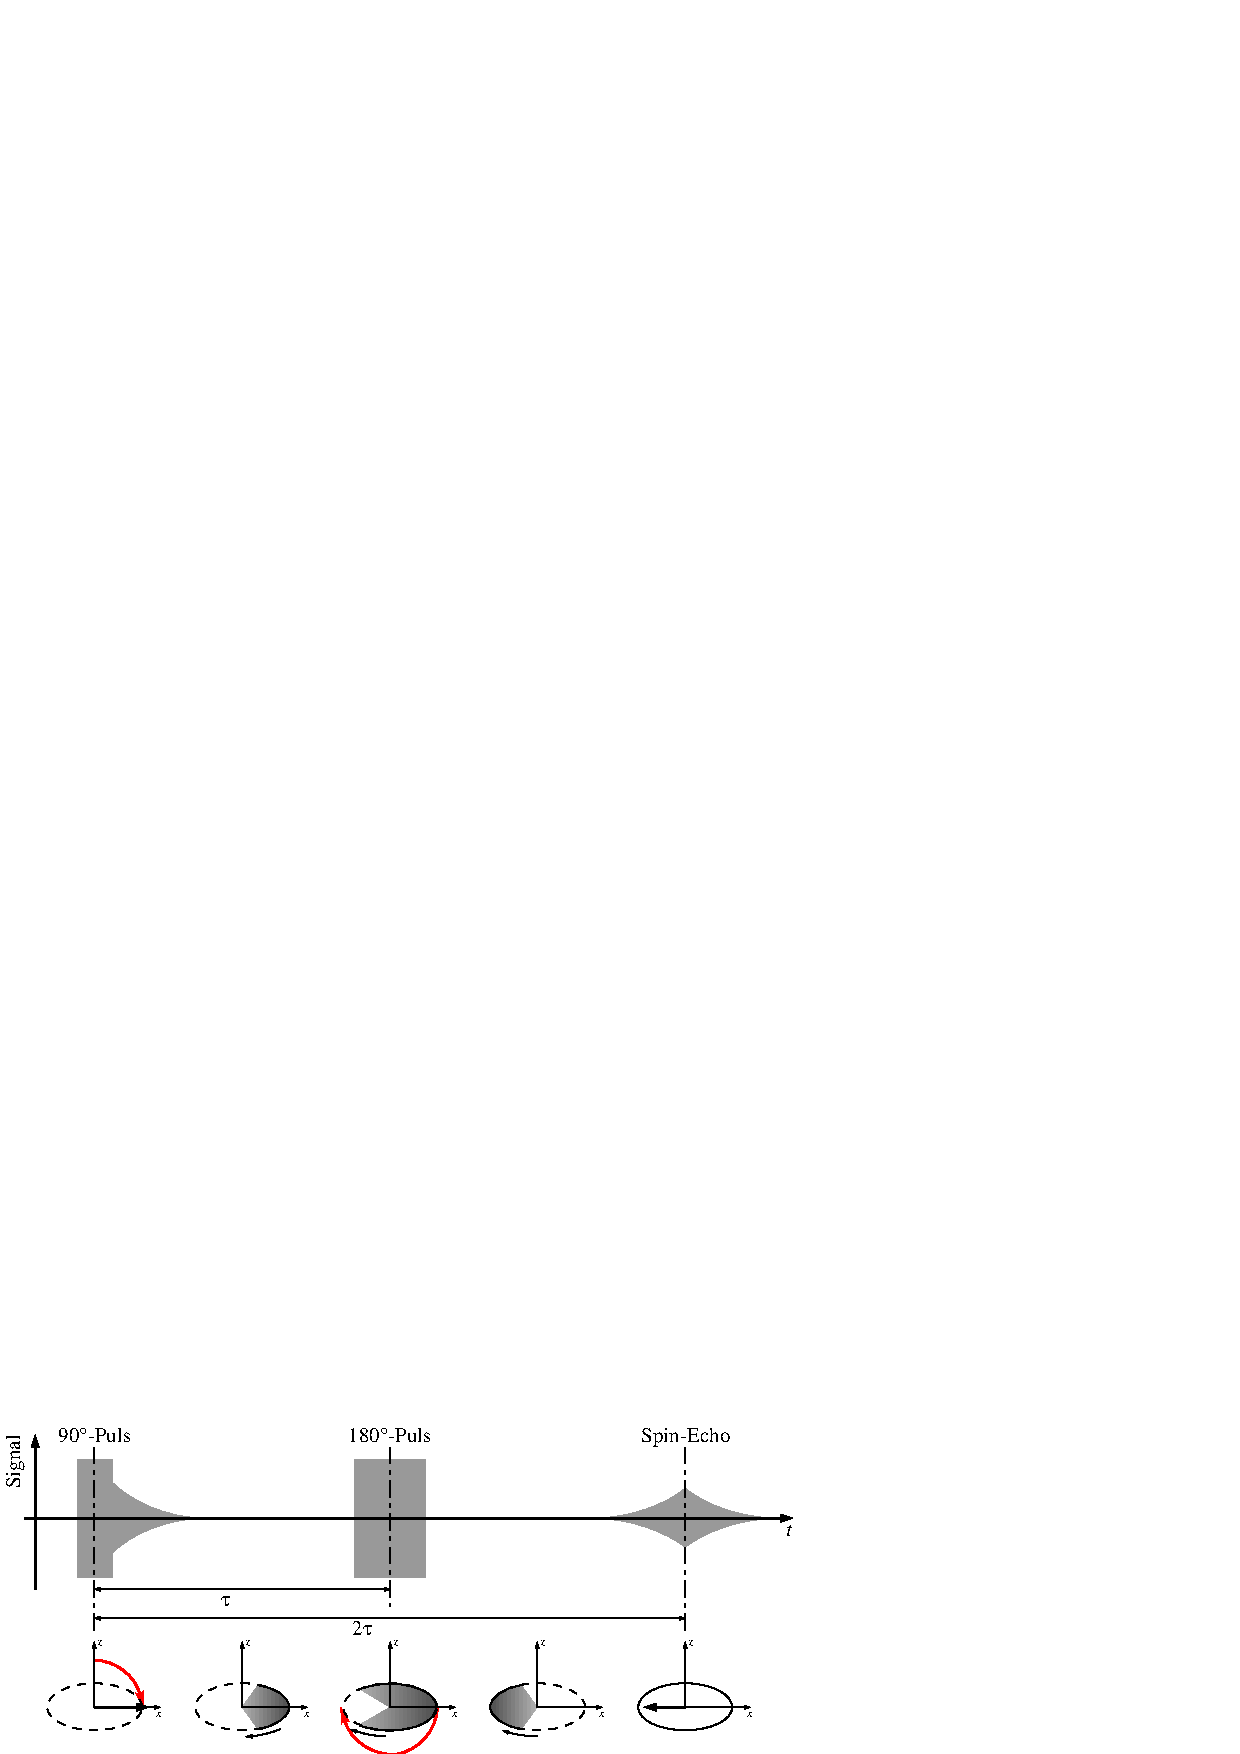
\includegraphics[bb=0 0 380 160]{drawings/T2Messung}$$
	\caption[Schema der Methode zur Messung der Spin"=Spin Relaxationzeit]{{\upshape\bfseries Schema der Methode zur Messung der Spin"=Spin Relaxationzeit} im
		mit einer mittleren Frequenz $\overline{\omega}$ rotierenden Koordinatensystem betrachtet.
		Dem ersten 90°"=Puls folgt nach variabler Verzögerung $\tau$ der 180°"=Puls, der das Feld
		der bereits auseinandergelaufenen, dephasierten Spins an der $yz$"=Ebene spiegelt und
		somit zu einer Fokussierung der Spins führt, die daraufhin zur Zeit $2\tau$ ein mit der
		Probenspule meßbares Echo erzeugen, das nur durch die intrinsische Dephasierung an
		Amplitude verloren hat.}
	\label{fig:t2methode}
 \end{figure}

Zur Messung der Spin"=Spin Relaxationzeit $T_2$ wurde nun gezielt die in der Frequenz höher
liegende, rechte Resonanzlinie des Isotops $^{71}$Ga angeregt (siehe Abb.~\ref{fig:t2messung}).
Hierbei muß man noch anmerken, daß sich die Probe bei dieser Messung nicht im Mittelpunkt der
Gradientenspule befand. Somit sind alle Frequenzen durch den konstanten Anteil des Gradienten, der
durch den Abstand der Probe vom Nullpunkt des Gradientenfeldes gegeben ist, leicht zu
höheren Frequenzen hin verschoben. Vor Einschalten des Gradientenfeldes lag die Resonanzlinie von
$^{71}$Ga bei 2.456~MHz, aber die Mittenfrequenz der Doppellinie bei vorhandenem
Magnetfeldgradienten ist 2.686~MHz. Aus der Differenz der beiden Frequenzen errechnet sich ein
mittleres Gradientenfeld an der Probe von
	\begin{equation}
		\Delta B_0 =
			\frac{2686\:\mathrm{kHz}-2456\;\mathrm{kHz}}{13.001\frac{\mathrm{kHz}}{\mathrm{mT}}} =
			18 mT \ttext{.}
	\end{equation}
Das heißt, daß die Spin"=Spin Relaxationzeit mit dieser Messung in einem Feld von ca.\ 207~mT bestimmt
wurde.

Für den 90° HF"=Puls wurde für eine Frequenz von $\nu=2.720$~MHz und eine Pulslänge von $1.47\;\mu$s
eine Abschwächung von 6 dB ermittelt. Der HF"=Pulser wurde so programmiert,
daß er das Analog"=Gate zuerst für 1.47~$\mu$s öffnet, dann für $\tau\;\mu$s schließt und dann wieder für
$2.94\;\mu$s öffnet. Diese Pulssequenzen wurden, um eine vollständige Relaxation der Spin"= und
Elektronentemperatur der Probe zu gewährleisten, mit einem zeitlichen Abstand von mindestens
$5T_1$ ausgeführt.

 \begin{figure}[htp]
	\begin{center}
		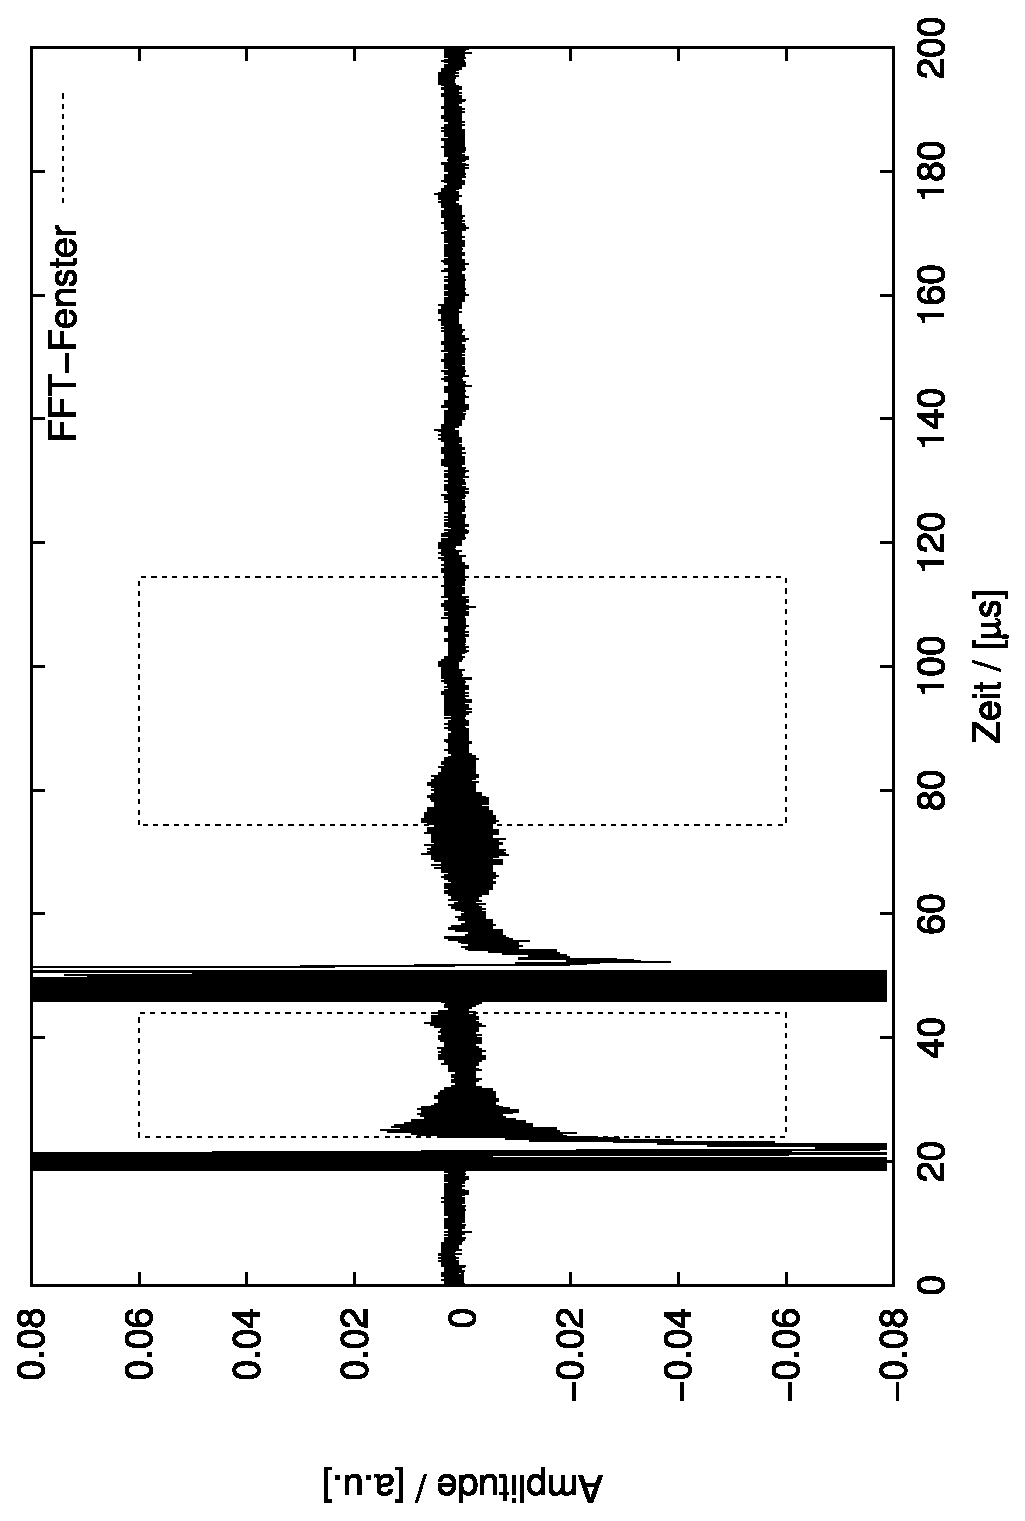
\includegraphics[angle=-90,width=\bigwidth]{plots/t2_auswert_shots_1}

		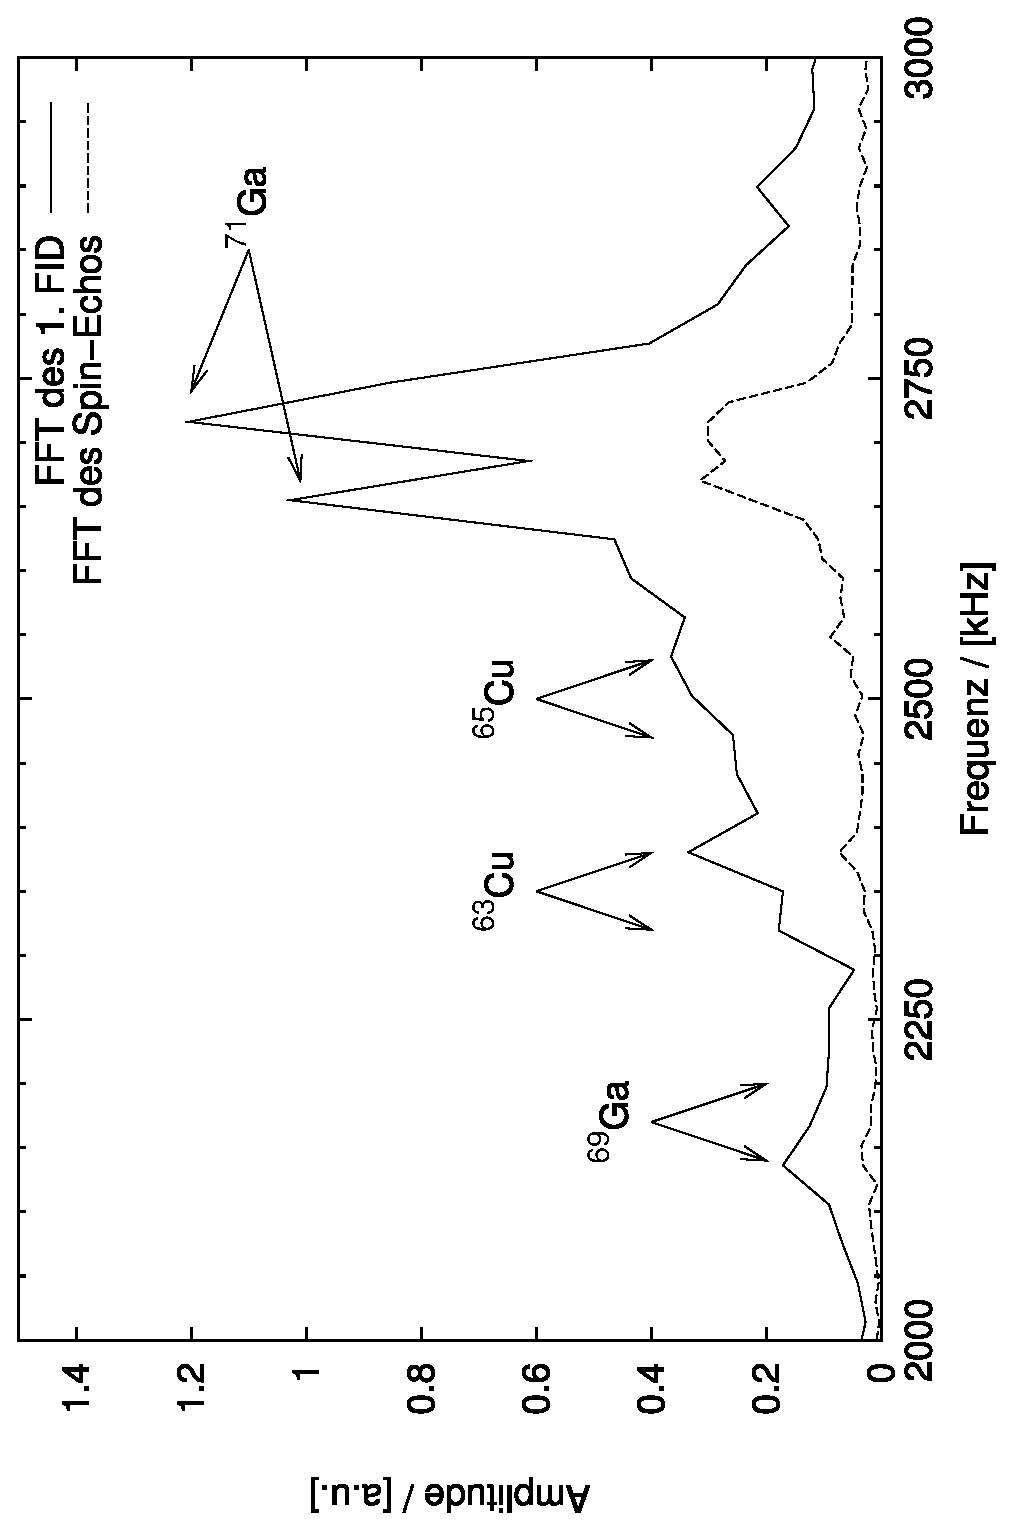
\includegraphics[angle=-90,width=\bigwidth]{plots/t2_auswert_shots_2}
	\end{center}
	\caption[Eine gemessene Pulssequenz der $T_2$"=Messung]{{\upshape\bfseries Eine gemessene Pulssequenz der $T_2$"=Messung.} Man sieht das
		Auftreten des Spin"=Echos, dessen Amplitude mit größerer Wartezeit $\tau$ kleiner wird. Die
		zur Bestimmung der Signalamplitude verwendeten Fenster, in denen eine Fouriertransformation
		des Zeitsignals durchgeführt wurde, sind gestrichelt eingezeichnet. In der
		Fouriertransformation des FID nach dem 1. 90° Puls im rechten Bild sieht man deutlich die
		Aufspaltung der Linie des $^{71}$Ga in die im Text beschriebene Doppellinie [{\bfseries
		Parameter:} $B_0$=207~mT, $\Delta B$=14$\frac{\mathrm{mT}}{\mathrm{cm}}$, $\nu$=2.720MHz,
		Pulslänge: 1.47~$\mu$s--$\tau$--2.94~$\mu$s, Abschwächung: 6 dB]}
	\label{fig:t2messung}
 \end{figure}

\subsubsection{Auswertung der $T_2$"=Messung}
Aufgrund der durch den Magnetfeldgradienten veränderten Linienform konnte keine Anpassung der
NMR"=Linien im Frequenzspektrum des FIDs nach dem 90° HF"=Puls und des Echos durchgeführt werden. 
Als Ersatz hierfür wurde die Amplitude der Resonanzlinie direkt aus dem Frequenzspektrum des
Echosignals ermittelt.

Aus der Blochgleichung~\eqref{eqn:bloch} ergibt sich ein exponentieller Zerfall der
Quermagnetisierung $M_\perp$ mit der Zeitkonstante $T_2$. Da die aus dem Frequenzspektrum des Echos
bestimmte Amplitude über die Änderungen des magnetischen Flusses durch die Probenspule proportional zur
Quermagnetisierung $M_\perp$ ist, kann man die Zerfallszeit $T_2$ daraus bestimmen.
Auf eine Normierung der aus dem Echospektrum erhaltenen Amplitudenwerte wurde verzichtet, da dies
für eine Bestimmung der Zeitkonstante des Zerfalls nicht nötig ist. Wenn man nun wie in
Abbildung~\ref{fig:t2ergebnis} zu sehen die gemessene Amplitude der Resonanzlinie über der
Zeit $2\tau$ aufträgt, kann man daran in logarithmischer Darstellung eine Gerade anpassen. Die
Zeitkonstante $T_2$ ergibt sich dann aus dem negativen Kehrwert der ermittelten Steigung der
Geraden. In diesem Fall erhält man 
$$\fbox{$T_2 = 39.6\pm0.7\;\mu$s.}$$

\begin{figure}[htp]
	\begin{center}
		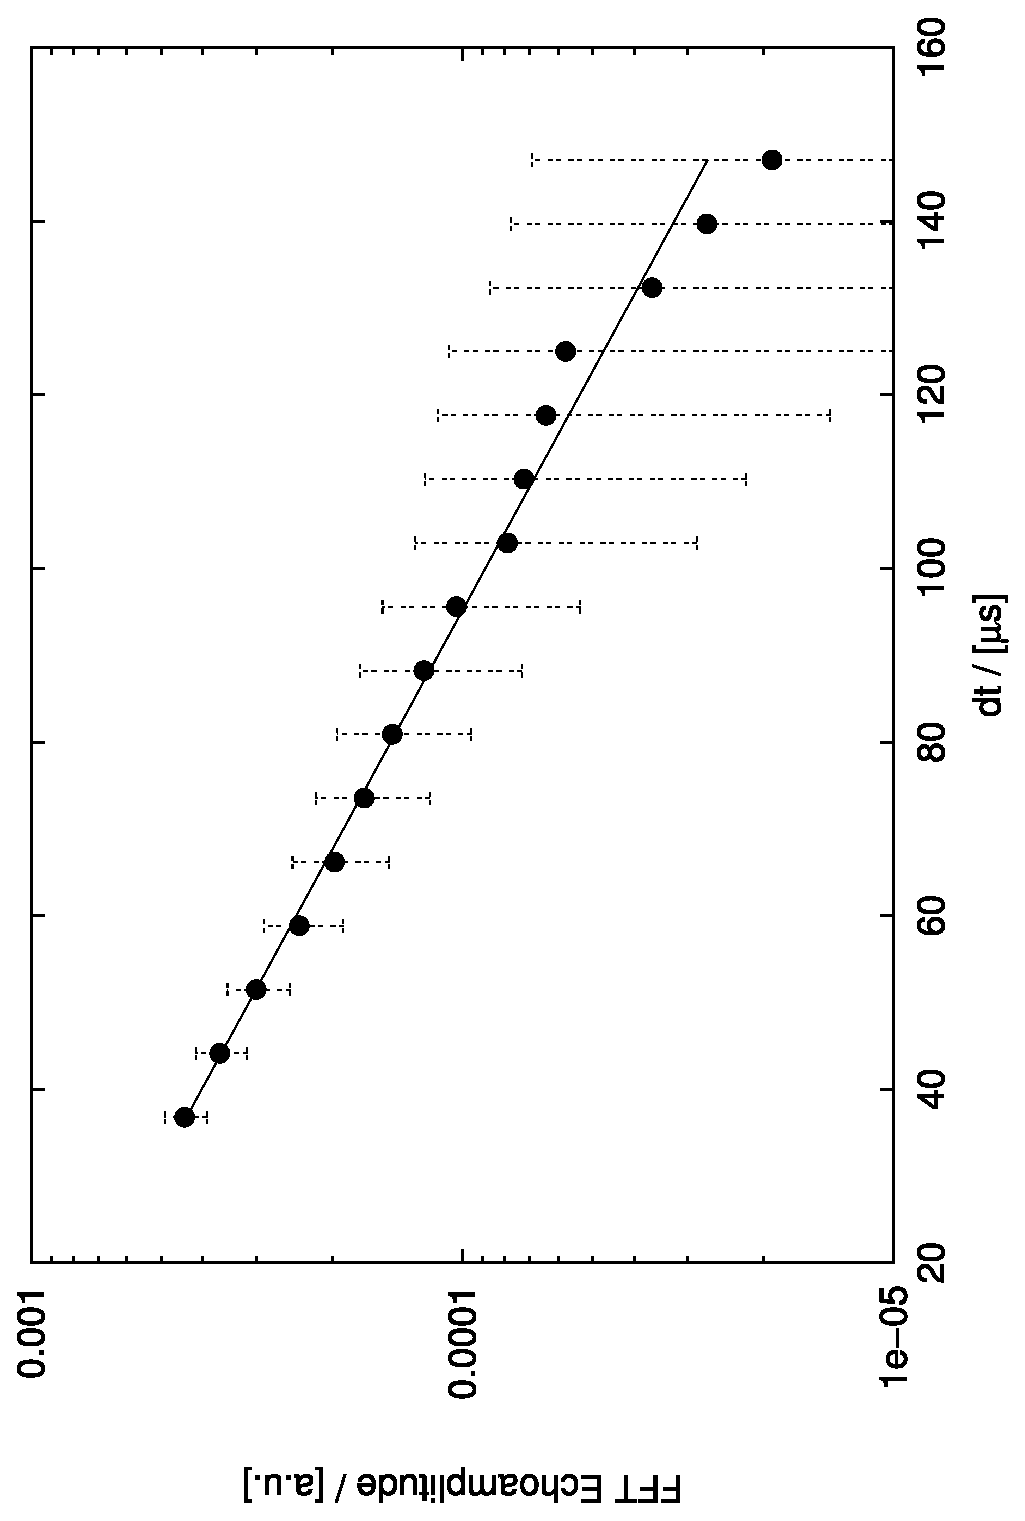
\includegraphics[angle=-90,width=\midwidth]{plots/t2_aug0897_4}
	\end{center}
	\caption[Ergebnis der $T_2$"=Messung]{{\upshape\bfseries Ergebnis der $T_2$"=Messung.} Diese Messung wurde bei einer
		konstanten Temperatur von 5 mK bei einem Magnetfeld $B_0$ von 207 mT durchgeführt. Aus
		der Anpassung der Geraden an die Meßdaten ergibt sich für $T_2=39.6\;µ$s}
	\label{fig:t2ergebnis}
 \end{figure}

\subsection{Frequenzverschiebung der NMR"=Linien}
Die aus der Anpassung der NMR"=Resonanzlinien mit hoher Genauigkeit erhaltenen Frequenzlagen der
Resonanzen kann man über die jeweilige Probentemperatur auftragen, wie in Abbildung~\ref{fig:frequenzshift}
zu sehen.

Die Polarisationen der Elemente Gallium und Kupfer besitzen aufgrund des in der gleichen Größenordnung
liegenden magnetischen Moments und des übereinstimmenden Kernspins von $\frac32$ eine ähnliche
Temperaturabhängigkeit. Deshalb sollte die Resonanzlinie des Kupfers der NMR"=Spule
zu tiefen Temperaturen hin, also bei steigender Polarisation, ein ähnliches Verhalten in der
Linienverschiebung wie die Linien der Galliumisotope zeigen, die ein Resultat der zunehmenden Magnetisierung
ist. Da dieses vorhergesagte Verhalten nicht eintritt, kann man folgern, daß die Kupferspule für
Temperaturen unterhalb von T>40~mK thermisch nur noch schlecht an die \aug"=Probe angekoppelt ist.
Wogegen man bei den Galliumlinien eine deutliche, mit der Polarisation zunehmende Linienverschiebung
erkennen kann.

Die in Abbildung~\ref{fig:frequenzshift} eingezeichneten mittleren Resonanzlinienpositionen für
eine Temperatur $T>40$~mK können zur Überprüfung der Knight"=Shift $\K$ herangezogen werden:
	$$\begin{tabular}{|r||c|c|c|}\hline
					& $^{63}$Cu	& $^{69}$Ga	& $^{71}$Ga	\\\hline
	$\nu$ / [kHz]	& 4640		& 4185		& 5318		\\\hline
	\end{tabular}$$
Aus der Position der Kupferlinie ergibt sich ein Feld von 410~mT an der Probe. Nun kann man die
Knightshift der Gallium"=Resonanzlinien aus
	\begin{equation}
		\gamma(1+\K)\,B=\nu\quad\Longrightarrow\quad\K=\frac{\nu}{\gamma\,B}-1
	\end{equation}
bestimmen. Man erhält nun für $\K(^{69}\mathrm{Ga})= -0.16$\% und $\K(^{71}\mathrm{Ga})=
-0.14$\%. Die Knight\-shift von $^{71}$Ga stimmt mit dem in \cite{AuGa2Dilemma} angegebenen Wert
überein.

 \begin{figure}[htp]
	\begin{center}
		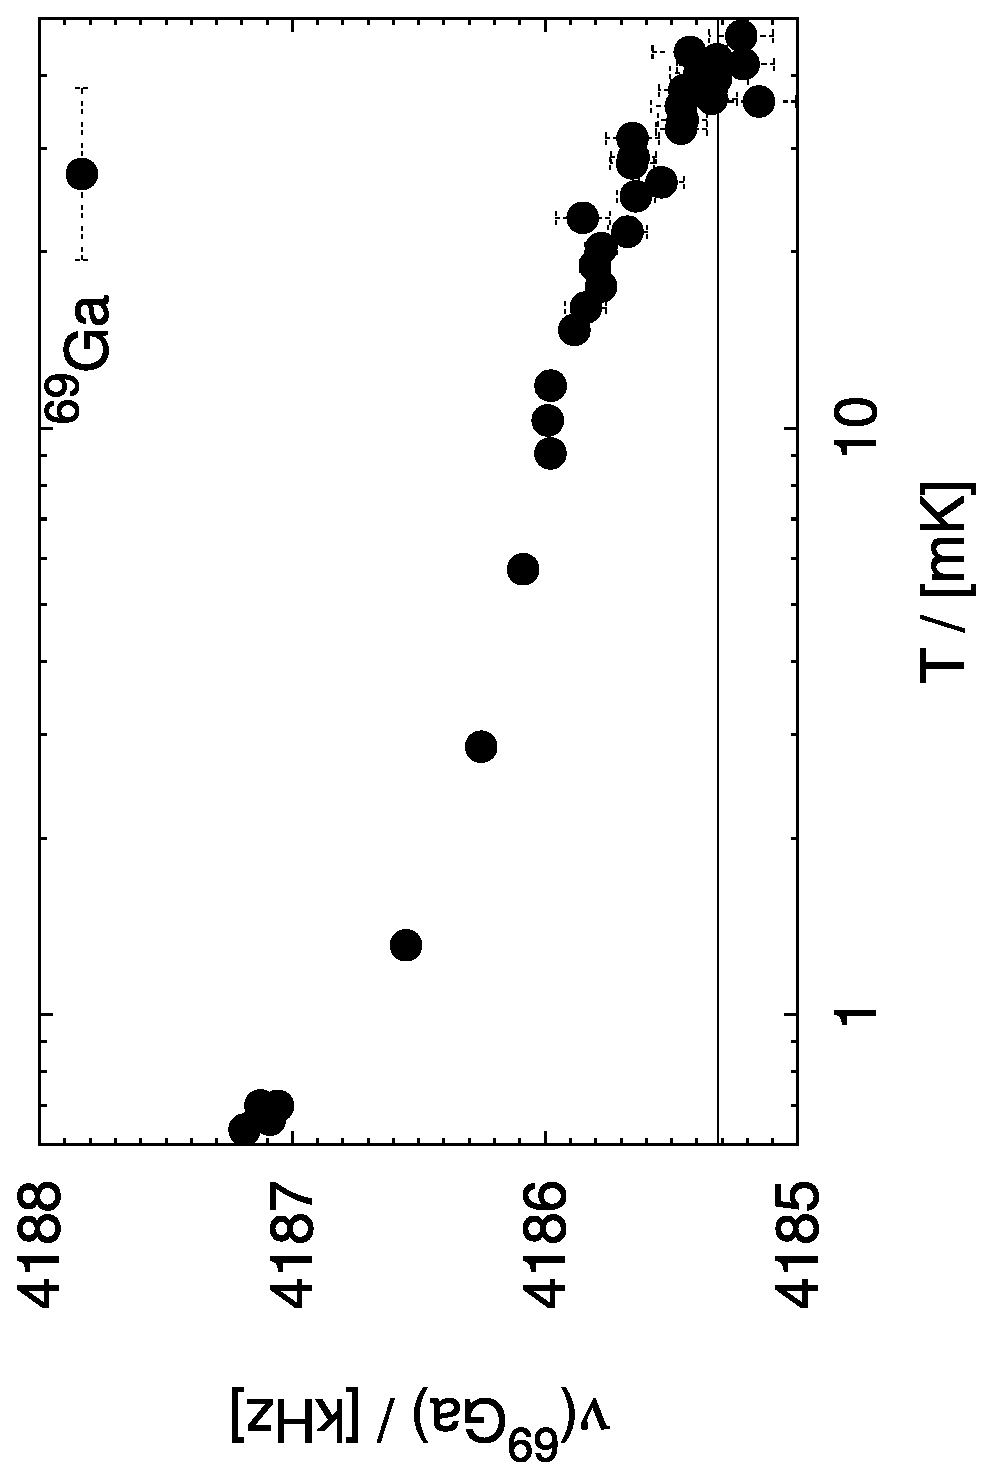
\includegraphics[angle=-90,width=\ssmallwidth]{plots/knight_aug1197da_3}\\
		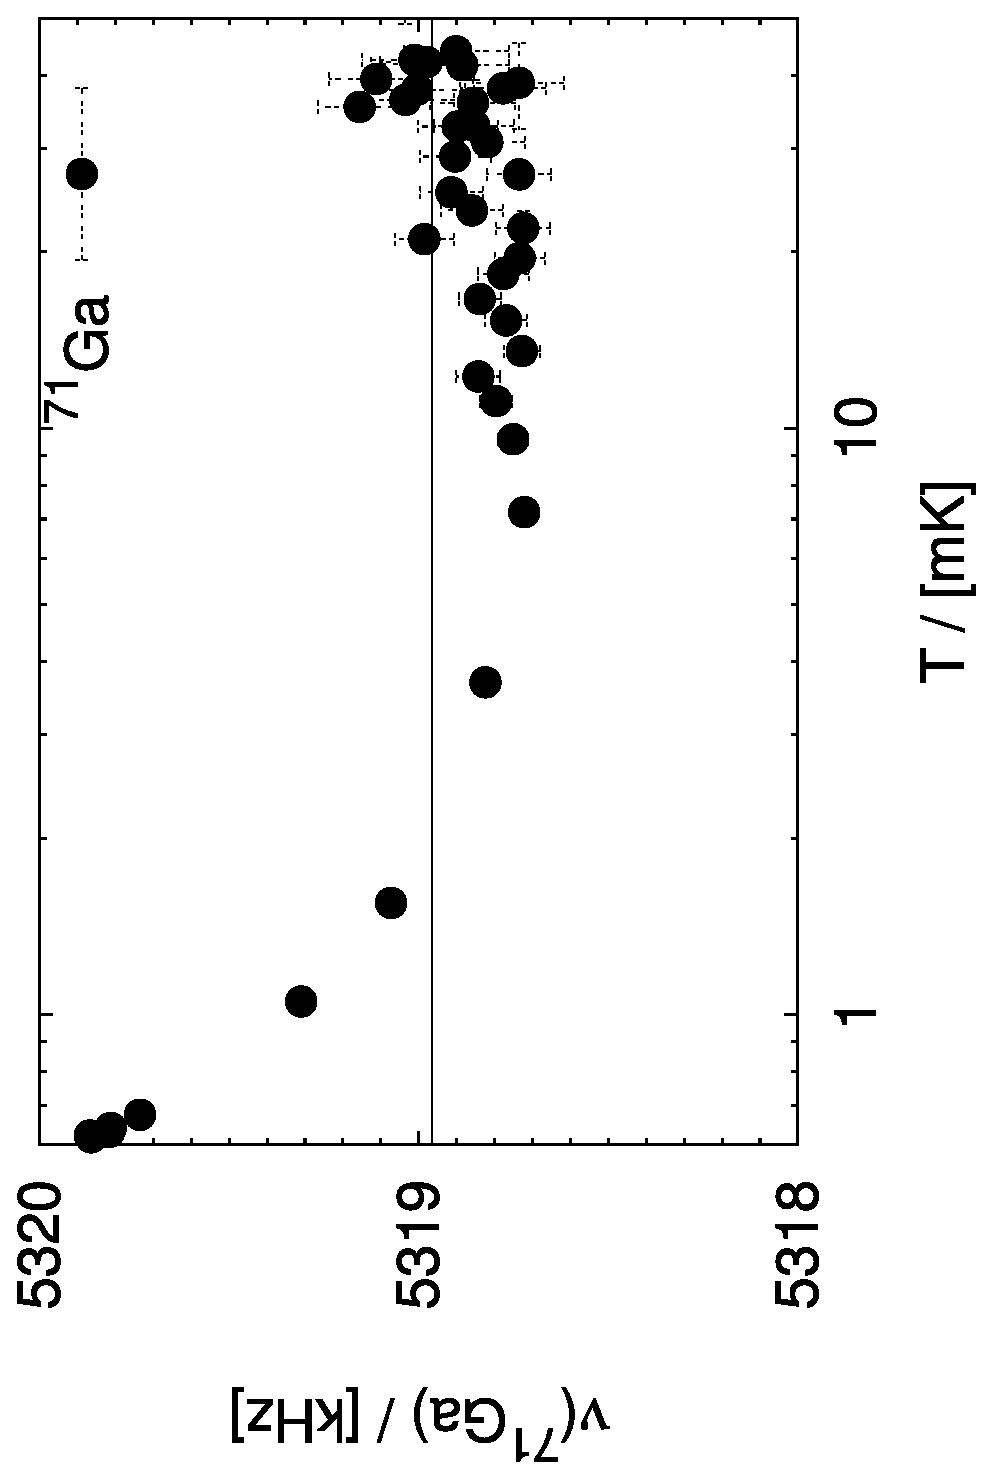
\includegraphics[angle=-90,width=\ssmallwidth]{plots/knight_aug1197da_4}\\
		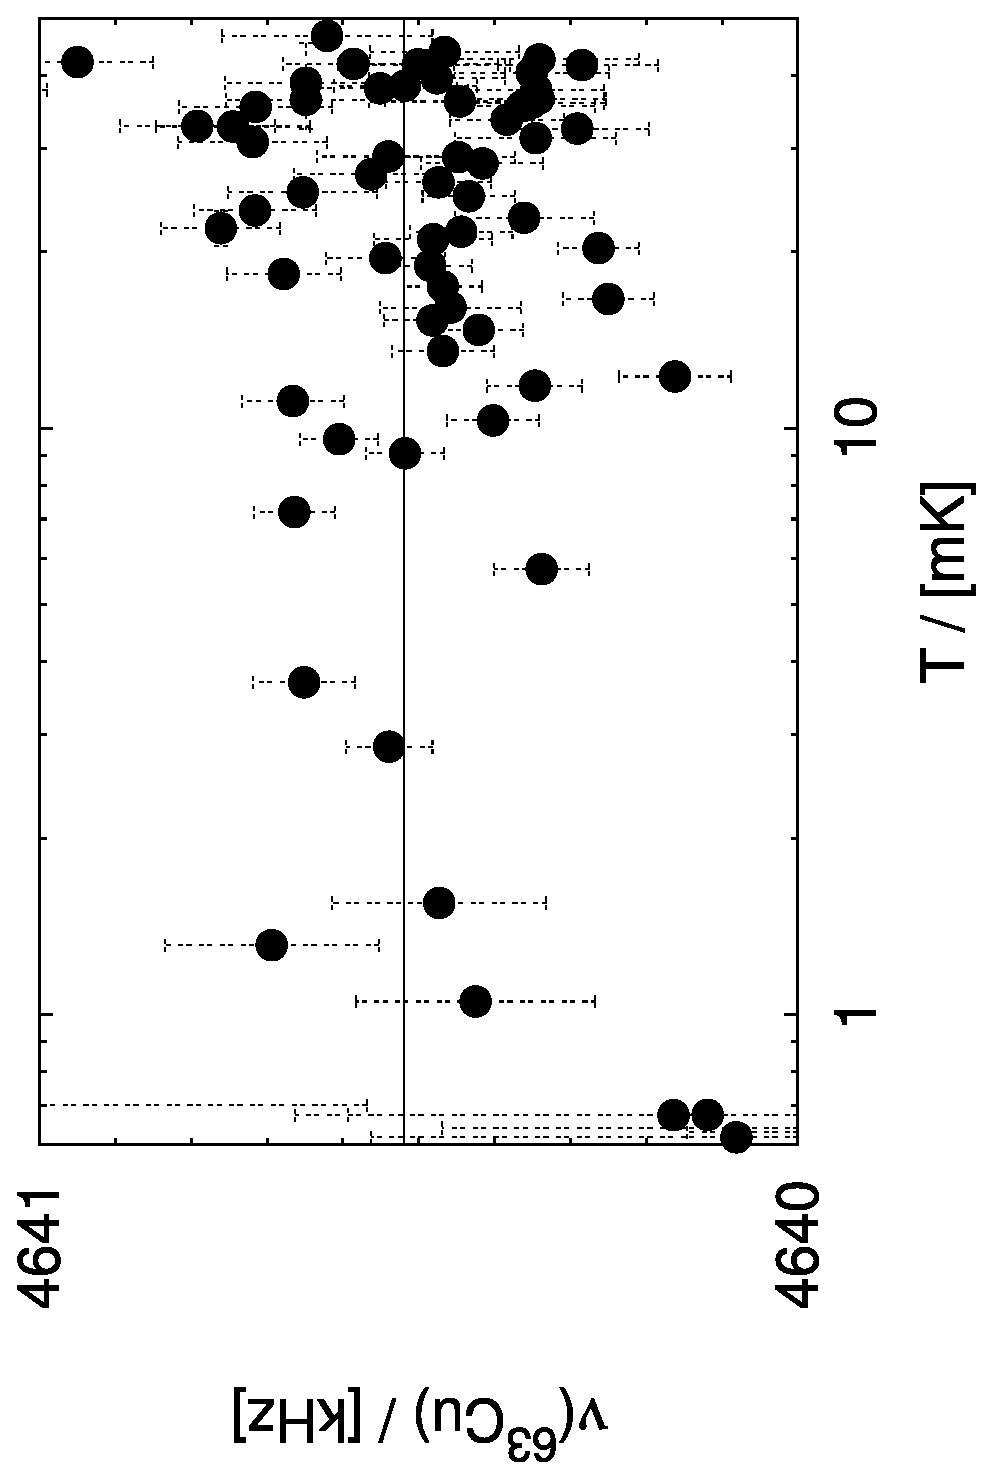
\includegraphics[angle=-90,width=\ssmallwidth]{plots/knight_aug1197da_5}\\
		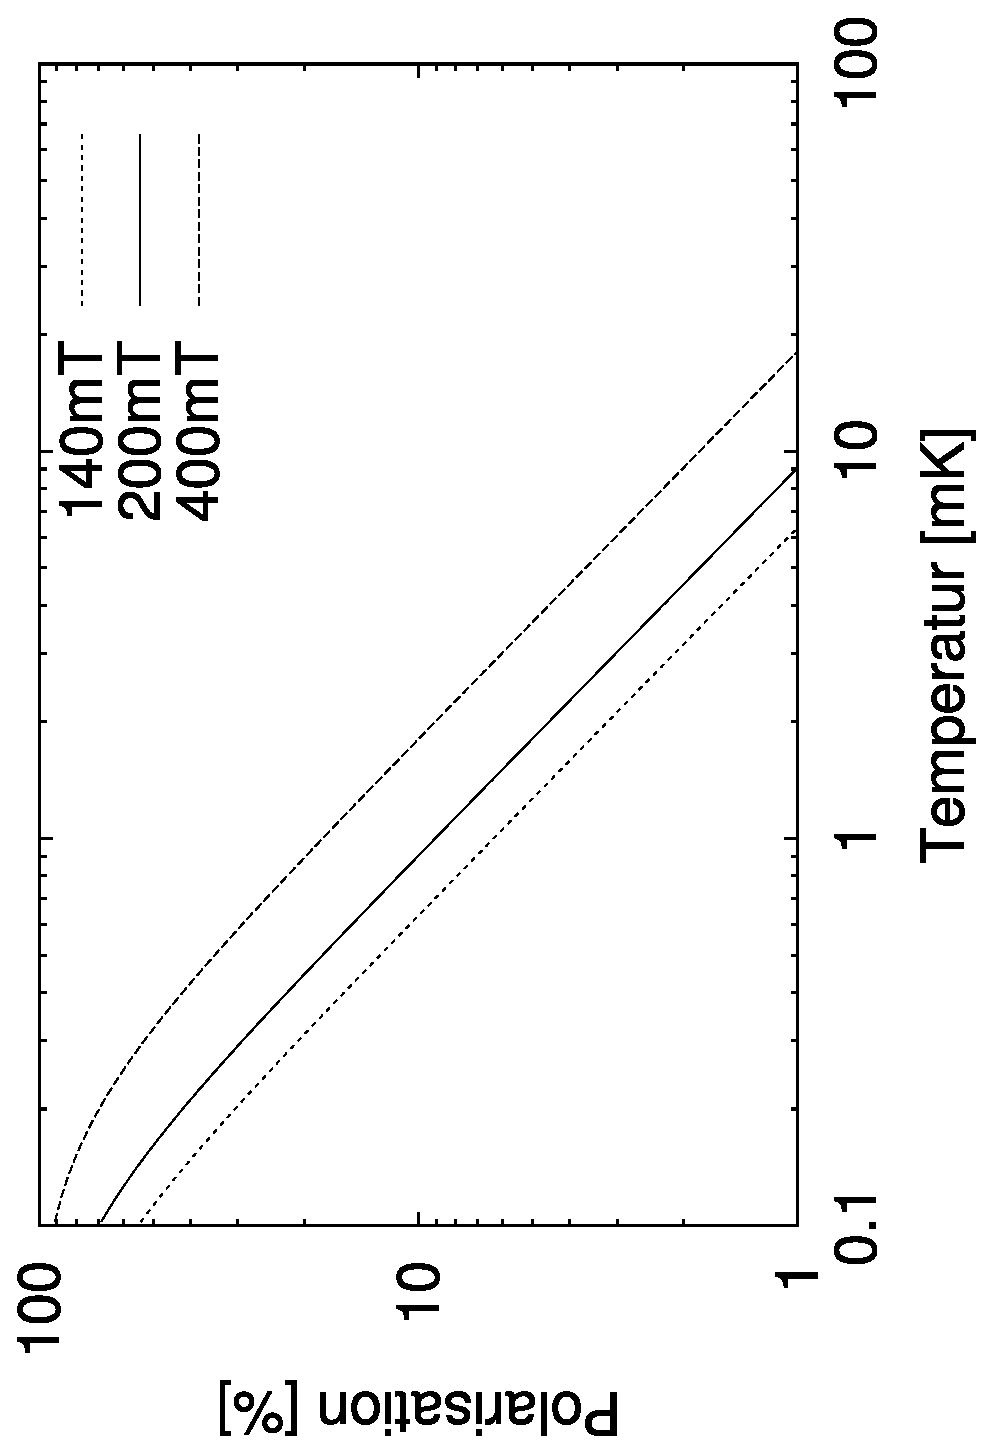
\includegraphics[angle=-90,width=\ssmallwidth]{plots/pol_ga}
	\end{center}
	\caption[Frequenzlagen der $^{69}$Ga"= und $^{71}$Ga"= und
		$^{63}$Cu"=Resonanzlinien]{{\upshape\bfseries Frequenzlagen der $^{69}$Ga"= und $^{71}$Ga"= und
		$^{63}$Cu"=Resonanzlinien.} Die mittleren Frequenzen für Temperaturen über 40 mK sind durch
		waagerechte Striche gekennzeichnet. Im Plot rechts unten ist der Verlauf der Polarisation
		von \aug{} bei tiefen Temperaturen für die in den durchgeführten Messungen verwendeten
		Magnetfelder dargestellt.}
	\label{fig:frequenzshift}
 \end{figure}

\section{Zusammenfassung und Diskussion der Ergebnisse}

Es wurde im Rahmen dieser Arbeit eine einphasige, polykristalline \aug"=Probe aus 6N$^+$ Ga und 5N$^+$Au hergestellt.
Die Charakterisierung ergab ein Restwiderstandsverhältnis von 210, und aus der Messung der
statischen Suszeptibilität konnte man die Konzentration der magnetischen Verunreinigungen ($\sim \mu_B$)
der Probe mit 1 ppm nach oben hin abschätzen.

Weiterhin wurde die Spin"=Gitter Relaxationzeit $T_1$ bei den Feldern 0.14 und 0.4 T und im
Temperaturbereich von 0.8 bis 60 mK gemessen:

	$$\begin{tabular}{|r||c|c|c|c|}\hline
		$B_0$ / [mT]	& 140	& \multicolumn{3}{c|}{400}\\\hline
		$T$ / [K]		& 5.5	& 5.6	& 17	& 60	\\\hline\hline
		$T_1(\ga)$		& 146.0	& 187.0	& 60.51	& 17.47	\\\hline
		$T_1(\gb)$		& 104.7	& 130.7	& 36.95	& 10.94 \\\hline
	\end{tabular}$$

Für die Spin"=Gitter Relaxationzeiten $T_1$ im Feld 400~mT ergab sich Korringaverhalten mit:
	$$\begin{tabular}{|r@{ = }l|}\hline
		$\kappa(\ga)$	& $1030\pm13$ mK s\\
		$\kappa(\gb)$	& $720\pm53$ mK s\\\hline
	\end{tabular}$$

In Spin"=Echo Experimenten ergab sich für $^{71}Ga$ im Feld $B=207$~mT für die Temperatur $T=5$~mK eine Spin"=Spin Relaxationzeit T$_2$ von
$39.6\pm0.7\mu$s.

Die Linienbreiten waren für beide Gallium"=Isotope im untersuchten Bereich feld"= und temperaturunabhängig.

Schließlich wurde die Knightshift von Gallium aus der Frequenz der Resonanzlinien und der
bekannten Knightshift von Kupfer bestimmt:
	$$\begin{tabular}{|r@{ = }l|}\hline
		\K(\ga)	& $-0.16$\%\\
		\K(\gb)	& $-0.14$\%\\\hline
	\end{tabular}$$

\subsubsection{Diskussion der Ergebnisse und Ausblick}

Das in \cite{Wagner_Dis} beschriebene NMR"=Verhalten von AuIn$_2$ konnte mit den im Rahmen dieser
Arbeit durchgeführten Messungen für \aug{} nicht beobachtet werden. 

In Übereinstimmung mit AuIn$_2$ ist die Verkürzung der Spin"=Spin Korrelationszeit $T_2$ um eine
Größenordnung. In der folgenden Tabelle sind die gemessenen NMR"=spezifischen Parameter zum Vergleich gegen
die von elementarem Gallium und AuIn$_2$ aufgetragen:
	$$
	\begin{tabular}{|r||c|c|c|c||c|c|}
	\cline{4-7}
	\multicolumn{3}{c}{}&
	\multicolumn{4}{|c|}{\bfseries Vergleich}\\
	\hline
	\rule[-1ex]{0cm}{3.5ex}&
		\multicolumn{2}{|c}{ Ga Einkristall}	&
		\multicolumn{2}{|c||}{AuGa$_2$}&
		AuIn$_2$	& In\\
	\cline{2-7}
	\rule[-1ex]{0cm}{3.5ex}&
		$^{69}$Ga	& $^{71}$Ga	&
		$^{69}$Ga	& $^{71}$Ga	&
		$^{115}$In	& $^{115}$In\\
	\hline\hline
	\rule[-1ex]{0cm}{3.5ex}$\kappa$/[Ks]	& 1.008	& 0.630	& 1.030	& 0.720	& 0.10	& 0.09\\\hline
	\rule[-1ex]{0cm}{3.5ex}T$_2$/[$\mu$s]	& 260	& 400	& ---	& 39.6	& 83	&$\approx$100\\
	\hline
		\multicolumn{1}{c}{}&
	\multicolumn{4}{|c|}{\footnotesize(bei $T\approx5$mK und $B\approx0.1$T)}&
	\multicolumn{2}{c}{}\\
	\cline{2-5}
	\end{tabular}$$

Weiterführende Messungen könnten zur genaueren Bestimmung der Temperaturabhängigkeit der Korringa"=Konstante $\kappa$
durchgeführt werden, da diese im Moment noch nicht geklärt ist. Eine andere mögliche Richtung der
Fortführung dieser Experimente ist die Herstellung weiterer, mit einer definierten Verunreinigung
versehener Proben, da ein Einfluß der Verunreinigungen auf das Verhalten der AuIn$_2$ Probe nicht
auszuschließen ist.

\appendix
\newpage
\addcontentsline{toc}{chapter}{\bibname}
\bibliography{Literatur}

\newpage
\listoffigures


%%%%%%%%%%%%%%%%%%%%%%%%%%%%%%%%%%%%%%%%%%%%%%%%%%%%%%%%%%%%%%%%%%%%%%%%%%%%%%%%%%%%%%%%%%%%%%%%%%
\end{document}
